\documentclass[12pt, a4paper, fleqn]{jreport}

\usepackage{graduatethesis}
\usepackage{listings,jlisting}
\usepackage{cite}
\usepackage{here}


\makeatletter
%\def\@cite#1{$\m@th^{\hbox{\@ove@rcfont #1)}}$}
\makeatother

\title{最大の移動時間を最小化する教室割当問題の\\定式化と求解}
\author{都11-23 岡崎 俊介}
\date{平成27年2月13日}
\西暦

\begin{document}
\maketitle
\setcounter{tocdepth}{2}
\setlength{\mathindent}{0zw}
\pagenumbering{roman}
\tableofcontents
\newpage
\pagenumbering{arabic}
\setcounter{totalnumber}{3}
\setcounter{topnumber}{3}
\renewcommand{\topfraction}{0.99}
\renewcommand{\bottomfraction}{0.99}
\renewcommand{\textfraction}{0.0}

\lstset{
  basicstyle={\ttfamily},
  breaklines=true,
  columns=[l]{fullflexible},
  lineskip=-0.5zw,
}

\setlength{\textwidth}{\paperwidth}   %%本文を用紙の横サイズにする
\addtolength{\textwidth}{-2in}         %それを2インチ引く
\setlength{\textheight}{\paperheight} %%本文を用紙の縦サイズにする
\addtolength{\textheight}{-2in}        %それを2インチ引く
\setlength{\topmargin}{0pt}            %ページ上端の余白を消す
\addtolength{\topmargin}{-\headheight} %(ページ上端の余白)-(ヘッダーの高さ)
\addtolength{\topmargin}{-\headsep}    %                  -(ヘッダーと本文の余白)
\setlength{\oddsidemargin}{0pt}       %%奇数(右)ページの左余白消す
\setlength{\evensidemargin}{0pt}      %%偶数(左)ページの左余白を消す



\chapter{はじめに}
人は,移動をする生き物である.
移動をして,様々な目的地へ赴き,やりたいこと,またはしなければならないことをする.
移動には,ピクニックのように移動そのものを楽しむ場合,すなわち移動そのものが目的である場合と,通勤や通学のように時間がもったいないが移動しなければならない場合,すなわち移動が別の目的のための手段となっている場合がある.

移動が別の目的のための手段となっている場合の1つに,大学内での教室移動がある.
大学内での教室移動は,授業と授業の間の休み時間に行うため,休み時間を移動に費やすことになる.
短い休み時間で休憩,及び授業の準備も行わなければならない学生にとっては,移動時間はできるだけ短いほうが望ましい.

通常,大学では授業によって開講される教室が異なっており,どの授業にどの教室を割り当てるかは手動で決めることが多い.
実際,現在関西大学においても,授業に対する教室の割当は全て手動で行われている.
また,関西大学では多くの学部が授業を開講するため,教室を割り当てる際に学生の移動時間まで考慮することは難しい.

この問題に似た問題として,大学における時間割作成の自動化が挙げられる.
この問題についての研究は数多く存在している.\cite{dadasenko,dadasan}.
そこで本研究では,一般的な割当問題\cite{ハンドブック}の枠組みの下で授業に対する教室の割当を自動化する手法を考えることにする.
このような問題を本研究では教室割当問題と呼ぶことにする.

教室割当の自動化については,例えば,マルチエージェントシミュレーションを行い,学生の移動時間を最小化した教室配置を行う研究がある\cite{kurousitemituketa}.
これに対し本研究では,移動時間が最小になる教室の割り当て方を求める.
具体的には教室割当問題を最適化問題として定式化し,最適化ソルバーを用いてそれを解くことを試みる.

実は\cite{先行研究}でも同じような研究が行われており,学生の移動時間の総和を最小化するような教室割当を求めることを目標とした最適化問題を解いている.
この最適化問題は,授業・教室・履修者の基本的なデータがあれば計算を行うことができるため,大学毎の授業システムに影響されず,多くの大学で使用可能な汎用性の高い教室割当が可能になる.
しかしながら,\cite{先行研究}の提案手法が大きな計算時間を要するものであり,最適解を求めることができないケースが多く見られた.

そこで本研究では,\cite{先行研究}とは目的を変更し,学生の移動時間の最大値を最小にするような教室割当を求めることを目指す.




\chapter{準備}

本章では,次章以降で必要となる事項について説明する.

\section{数理計画問題}

数理計画問題は以下のように表すことができる\cite{数理計画入門}:\\
         目的関数 : $f(x)$ → 最小(あるいは最大)\\
         制約条件 : $ x \in S$\\
ここで,$x$は$n$次元実ベクトル,目的関数$f$は$R^n$($n$次元実ベクトル空間)上で定義された実数値関数である.
また制約条件を満たす$x$を実行可能解,その集合である$S \subseteq R^n$を実行可能領域,実行可能解のなかで目的関数$f(x)$が最小(あるいは最大)となるものを最適解という.
このような問題を総称して数理計画問題(最適化問題)という.

\section{分枝限定法}

分枝限定法とは組合せ最適化問題の解を見つける方法の1つである\cite{数理計画入門, ハンドブック}.
組合せ最適化問題は有限個の要素からなる実行可能領域のなかで目的関数が最小となる解を見つける問題である.
実行可能解は有限個であるから,それらすべてを列挙することにより,最適解を求めることができる.
しかしながら,変数の数が多い場合,組合せの数が膨大になるため,すべての実行可能解を比較する方法では最適解を求めるのは難しい.

これに対し,分岐限定法は組み合わせ最適化問題の最適解を効率的に見つけるための方法のひとつである.
分枝限定法において,実行可能解を列挙するために場合分けを行っていく過程で,最適解が得られる見込みのない不必要な場合分けをできるだけ省略して探索する範囲を絞り込み,計算時間の短縮を図る.
分枝限定法の探索の方法を以下に記述する.
ここで,下界値とは最適値以下であることがわかっている値であり,上界値とは最適値以上であることが分かっている値である.

\begin{itembox}[l]{分枝限定法}
\begin{description}
\item[ステップ1] 適切な方法で初期実行可能解を求め,それを暫定解$x$とする.
暫定解$x$の目的関数値を$z$とする.
問題の集合${\cal N}={P_0}$とする($P_0$は原問題である).
\item[ステップ2] ${\cal N}=0$ならば,暫定解$x$を最適解として出力し終了.\\
そうでなければ,${\cal N}$から適当な子問題を選びそれを$P'$とし,${\cal N}$から$P'$を取り除く.
\item[ステップ3] $P'$の緩和問題を解き,得られた解を$\bar{x'}$,上界値を$\bar{z'}$とする.
緩和問題が許容解をもたないならばステップ2へ.
\item[ステップ4] $\bar{x'}$が元問題$P_0$の実行可能解かつ$\bar{z'}>z$の場合.\\
(原問題$P_0$の,より良い許容解が得られたので)$x:=\bar{x'}$,  $z:=\bar{z'}$と更新する.
ステップ2へ.
\item[ステップ5] $\bar{z'} \leq z$の場合.\\
(子問題$P'$の最適解は$x$より目的関数値が大きくないので)ステップ2へ.
\item[ステップ6] ($\bar{x'}$が元問題$P_0$の実行可能解でない,かつ$\bar{z'} > z$の場合)\\
$P'$の実行可能領域を分割した子問題を生成し,それらを${\cal N}$に加え,ステップ2へ.
\end{description}
\end{itembox}


\section{割当問題}

まず,割当問題の説明を行う際に必要となるマッチング問題について説明する.
マッチング問題とは,複数の仕事と複数の機械を1対1に対応させたり,何人かの人を2人ずつのグループに分けたりするように,対象物のペアを作る問題である.
この問題は,無向グラフ上でモデル化できる.
モデル化する際に,対象を頂点とし,ペアリング可能な頂点同士を無向枝で結ぶ.
ここで,ペアを作る枝の集合をマッチングという.
このようにして,要素数最大のマッチングか,各枝に与えられた費用の和が最小となる条件を満たすマッチングを求める問題をマッチング問題という.
そして,マッチング問題の中でも,2部グラフの最小費用マッチング問題を割当問題\cite{ハンドブック}と呼ぶ.
例えば,能力が異なる各社員にどの作業を割り当てると最もコストが少なくなる(もしくは最も利益を上げることができる)のかを求める問題を考える.
その例を図\ref{fig:wariate}に示す.
この図の点線はマッチング可能なペアを表しており,実線はマッチングを表している.
すなわち,社員a1が仕事b2, b3に割り当てられ,社員a2が仕事b4に割り当てられ,社員a3が仕事b1に割り当てられている\cite{ハンドブック}.
\begin{figure}[h]
\centering
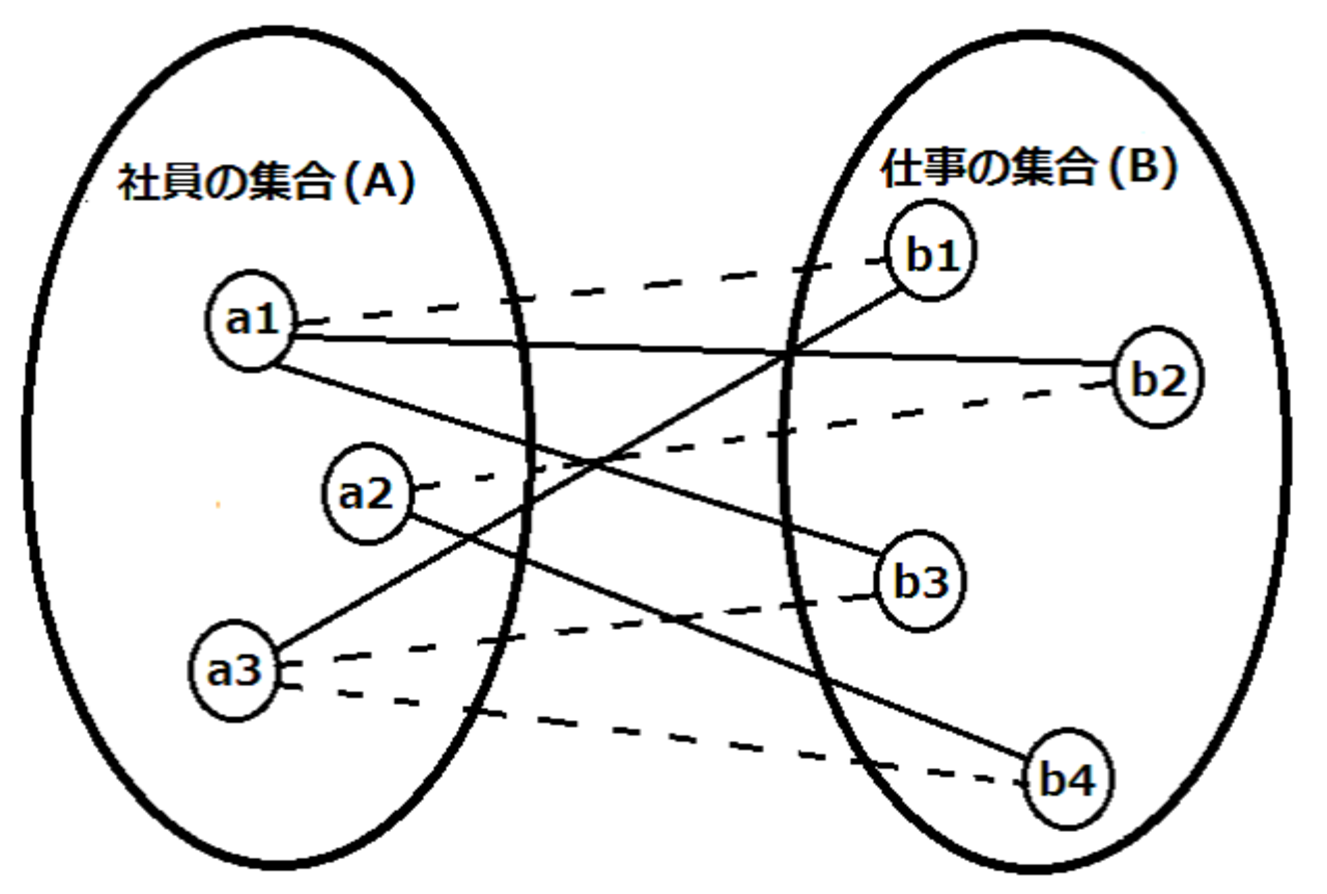
\includegraphics[width=10cm, clip]{wariate.eps}
\caption{割当問題の例}
\label{fig:wariate}
\end{figure}



\section{重み付き制約充足問題(WCSP)}

制約充足問題 (Constraint Satisfaction Problem, CSP)とは,変数の集合,変数領域の集合,制約の集合によって構成され,すべての制約を満たすように各変数に変数領域から値を割り当てる問題である.
このとき,すべての制約が満たされた解を実行可能解と呼ぶ.
一方,WCSP (Weighted CSP)\cite{CSP}では重要な制約条件をなるべく満足するためには値をどのように割り当てるとよいかを決定する問題であり,すべての制約を満たす必要はなく,制約条件の重要度を重みとして設定することができる.
そのため,制約条件は大きく2種類に分類することができる.
1つが絶対制約で,これは必ず成立させなければならない制約条件である.
よって,この制約が1つでも成り立っていない解は実行可能解とは言えない.
もう1つが考慮制約で,これは成立させることが好ましい制約条件である.
この制約が成り立っていない解も実行可能解と言える.
このとき,各考慮制約毎に違反ポイントを設定し,その総和を目的関数として,それを最小化する.


\section{最適化ソルバー}

最適化ソルバーは,数理計画問題の最適解を得るためのプログラムである.
これを利用するためにはまず,数理計画問題の定式化を行い,次に定式化した問題をモデリング言語で記述する.
最適化ソルバーによって利用できるモデリング言語は異なる.
そして,記述した問題を最適化ソルバーで読み込み,解を得る.
ここで,本研究で用いる最適化ソルバーGLPK\cite{GLPK}とIBM ILOG CPLEX Optimizer\cite{CPLEX}について説明する.

まずGLPKとは,GNU Linear Programming Kit の略で,GNUが無料配布しているソルバーである.
GLPKは,モデリング言語として,最適化の分野で広く用いられているモデリング言語AMPL (A Mathematical Programming Language)\cite{AMPL}のサブセット言語であるGMPLを採用している.
このソルバーは最適化計算を行うだけではなく,GMPL形式で書かれたモデルとデータを用いて,LP形式のファイルを作成することができる.

また,IBM ILOG CPLEX Optimizer\cite{CPLEX}とは,計算速度に定評のある最適化ソルバーの1つである.
モデリング言語はOPLを採用している.
そして,大規模な線形計画(LP),2次計画(QP),整数計画(IP),混合整数計画(MIP)を解くことができる.

本研究では,GLPKによって,GMPL形式で書かれたモデルとデータを,LP形式のファイルへ変換し,IBM ILOG CPLEX Optimizerを用いて計算を行っている.



\chapter{先行研究の概要}
本研究では,最大の移動時間を最小化する教室割当問題を行うが,これは先行研究\cite{先行研究}を参考にしたものである.
本章では,\cite{先行研究}の概要について説明する.
\section{背景}
現在,関西大学では手動で教室割当を行っている.
関西大学には約3万人の学生が在籍しており,約12000の授業がある.
このような多数の学生と授業を手動で処理し,移動時間を最小化する教室割当を行うことは非常に困難である.
また,休み時間には多くの学生が同時に移動するため,学生の動きを考慮した教室割当を行わなければ移動時に混雑が発生することがある.
さらに,現在の関西大学の休み時間は10分と短く,連続して授業を持つ学生や教員は,次の授業への移動と準備を時間内に行うことが困難なことがある.
そこで,先行研究では次のことを目標としていた.\\
\begin{center}
\fbox{
\begin{tabular}{c}
各授業の開講曜限が定められているとき,休み時間における全学生の\\移動時間の総和が最小となるような,授業に対する教室の割当を求めよ.
\end{tabular}
}
\end{center}
\vspace{5.0mm}
すなわち,先行研究では本大学の教室割当を自動化するとともに,余裕を持って移動を行えるように各学生の移動時間の総和を最小化する最適化問題を定式化し,求解を行った.

先行研究では各時限間の教室移動時間を最適化対象としているが,1,2限(午前)と3,4,5限(午後)の間には昼休みがあり,長い休みとなるので,移動時間を最小化する必要性はないと考えている.
そこで,先行研究では一日を午前・午後に分けて最適化を行っている.
さらに一週間は月曜から土曜の6日間,そして一年は春,秋の学期に分けられるので,最適化の対象は合計24通りとなる.

\if0
\section{解法}
先行研究では,移動時間が最小になることを考慮した教室割当問題を数理計画問題として定式化し,既に作成されている時間割のデータを用いて求解している.
具体的には,教室割当問題を重み付き制約充足問題(WCSP)として扱っている.
%具体的に得られる解が教室割当として成り立たせるために不可欠となる制約を絶対制約(必ず守るべき制約),より良い組み合わせを生むための制約を考慮制約(できるだけ守りたい制約)として扱っている.
また,先行研究では,定式化した数理計画問題を解くために,厳密解法を用いている.
厳密解法とは,最適化問題に対して,最適性の保証された解(最適解)を求める解法のことである.
厳密解法には,混合整数計画問題に対する分枝限定法,分枝価格法などがある.

\fi


\section{問題の定式化}
先行研究では以下のように教室割当問題を定式化して最適化を行っている.
\begin{itemize}
\item 集合と添字・パラメータ・変数
\begin{itemize}
\item 集合・添字\\
\begin{tabular}{ll}
$p \in P$    &: 時限とその集合\\
$j \in J$    &: 授業とその集合\\
$j \in J1_p$ &: $p$限目に開講される授業とその集合\\
$j \in L$    &: 特別連続授業とその集合\\
$(i,j) \in D$&: 特定の教室を指定する特定の授業の組とその集合\\
$i \in I$    &: 教室とその集合\\
\end{tabular}
\item パラメータ
\[
\begin{array}{rcl}
b & = &
\begin{array}{ll}
\mbox{休み時間の長さ} 
\end{array}
\\
m_{i} & = & 
\begin{array}{ll}
 \mbox{教室$i$の定員数} 
\end{array}
\\
n_{j} & = & 
\begin{array}{ll}
 \mbox{授業$j$の受講者数} 
\end{array}
\\
y & = & 
\begin{array}{ll}
 \mbox{混雑が起きる可能性が高まる移動時間} 
\end{array}
\\
q_{i_1,i_2} & = & 
\begin{array}{ll}
 \mbox{授業$i_1$と授業$i_2$の双方を受講する学生数} 
\end{array}
\\
r & = & 
\begin{array}{ll}
 \mbox{全ての移動で可能な限り守りたい移動時間} 
\end{array}
\\
t_{i_1,i_2} & = & 
\begin{array}{ll}
 \mbox{教室$i_1$と教室$i_2$間での所要移動時間} 
\end{array}
\\
z & = & 
\begin{array}{ll}
 \mbox{混雑が起きると予測される人数} 
\end{array}
\\
d_{j_1,j_2} & = & \left\{ 
\begin{array}{ll}
	1, & \mbox{$p$限目に授業$j_1$を,$(p+1)$限目に授業$j_2$を受講する学生が存在するとき} 		\\
	0, & \mbox{それ以外}
\end{array}
\right. \\
e_{p,j} & = & \left\{ 
\begin{array}{ll}
	1, & \mbox{時限$p$時に授業$j$が割り当てられているとき} 		\\
	0, & \mbox{それ以外}
\end{array}
\right. \\
f_{i_1,i_2} & = & \left\{ 
\begin{array}{ll}
1, & \mbox{$t_{i_1,i_2}\leq y$であるとき} \\
0, & \mbox{それ以外}
\end{array}
\right.\\
g_{i_1,i_2} & = & \left\{ 
\begin{array}{ll}
1, & \mbox{$t_{i_1,i_2}>r$であるとき} \\
0, & \mbox{それ以外}
\end{array}
\right.\\
h_{j} & = & \left\{ 
\begin{array}{ll}
1, & \mbox{$p$限目に授業を持たず,$(p+1)$限目に授業$j$を受講する学生が存在するとき} \\
0, & \mbox{それ以外}
\end{array}
\right.\\
\end{array}
\]
\vspace{3.0mm}
\item 変数\\
\vspace{-5.0mm}
\[
\begin{array}{rcl}
v_{i_1,i_2} & = & 
\begin{array}{ll}
\mbox{ある時限に教室$i_1$で授業が開講され,}\\
\mbox{その次の時限に教室$i_2$で授業が開講されているとき,その両方を受講している学生数}\\ 
\end{array}
\\
 u_{i,j} & = & \left\{ 
\begin{array}{ll}
1, & \mbox{教室$i$に授業$j$が割り当てられているとき} \\
0, & \mbox{それ以外}
\end{array}
\right. 
\\
w_{p,i_1,i_2} & = & \left\{ 
\begin{array}{ll}
1, & \mbox{$p$限目に教室$i_1$で授業が開講され,}\\
& \mbox{$(p+1)$限目に教室$i_2$で授業が開講されるとき}\\ 
0, & \mbox{それ以外}
\end{array}
\right.
\\
\alpha_{j_1,j_2} & = & \left\{ 
\begin{array}{ll}
1, & \mbox{特別連続授業$j_1,j_2$が異なる教室で開講されるとき}\\
0, & \mbox{それ以外}
\end{array}
\right.
\\
\beta_{j_1,j_2} & = & \left\{ 
\begin{array}{ll}
1, & \mbox{授業$j_1,j_2$間での移動時間ができるだけ守りたい指定の時間を越えるとき}\\
0, & \mbox{それ以外}
\end{array}
\right.
\\
 \delta_{i,j_1,j_2} & = & \left\{ 
\begin{array}{ll}
1, & \mbox{$p$限目に授業$j$を受講していて,$(p+1)$限目に授業$j_2$を受講せずに}\\
& \mbox{退室する学生集団と$p$限目に授業$j_1$を受講していて,}\\
& \mbox{$(p+1)$限目に授業$j_2$を受講するために入室してくる学生集団か,}\\
& \mbox{$p$限目に授業を持たず$(p+1)$限目に授業$j_2$を受講するために入室する}\\
& \mbox{学生集団で出入りのタイミングが合い,混雑が起きる可能性が高いとき}\\
& {出入りのタイミングが合い,混雑が起きる可能性が高いとき}\\
0, & \mbox{それ以外}
\end{array}
\right.
\end{array}
\]
\end{itemize}


\item 制約条件
\begin{itemize}
\item{変数を定義する制約条件}
\begin{itemize}
\item $v_{i_1,i_2}$\\
\begin{eqnarray}
\label{shensu-1} 
&&( u_{i_1,j_1} + u_{i_2,j_2} - 1 ) \cdot q_{j_1,j_2} \leq v_{i_1,i_2}\\
&&\hspace{20.0mm} \left(\forall p \in P,\: \forall i_1 \in I,\: \forall i_2 \in I,\:\forall j_1 \in J1_p,\:\forall j_2 \in J1_{p+1},d_{j_1,j_2}=1\right)\nonumber 
\end{eqnarray}
\item $w_{p,i_1,i_2}$\\
\begin{eqnarray}
\label{shensu-2} 
&& u_{i1,j1} + u_{i2,j2} - 1  \leq w_{p,i_1,i_2}\\
&&\hspace{20.0mm} \left(\forall p \in P,\: \forall i_1 \in I,\:\forall i_2 \in I,\:\forall j_1 \in J1_{p},\:\forall j_2 \in J1_{p+1},\:d_{j_1,j_2}=1\right)\nonumber 
\end{eqnarray}
\end{itemize}
\vspace{3.0mm}
\item{絶対制約}\\
\vspace{-3.0mm}
\begin{itemize}
\item {\bf[絶対制約1] : 1つの曜限における各教室には2つ以上の授業を割り当てられない.}\\

\vspace{-5.0mm}
 同じ曜限において,各教室に2つ以上の授業が割り当てられないようにするため,
教室$i$について,次の制約を与える:

\vspace{-3.0mm}
\begin{eqnarray}
\label{szettai-1}
&&\sum_{j \in J} u_{i,j} \cdot e_{p,j} \leq 1 \hspace{5.0mm}
\quad \left (\forall p \in P, \:\forall i \in I \right)
\end{eqnarray} 

\vspace{5.0mm}
\item {\bf[絶対制約2] : 各授業には必ず1つの教室を割り当てなければならない.}\\

\vspace{-5.0mm}
 ある曜限に存在する1つの授業に対して2つ以上の教室を割り当てないようにするため,
また,1つの授業に1つも教室が割り当てられないことを防ぐため,
授業$j$について,次の制約を与える:

\vspace{-3.0mm}
\begin{eqnarray}
\label{szettai-2}
&&\sum_{i \in I} u_{i,j}=1 \quad \left (\forall j \in J \right)
\end{eqnarray} 

\vspace{5.0mm}
\item {\bf[絶対制約3] : 受講人数が教室の定員を超えて教室に授業を割り当ててはいけない.}\\

\vspace{-5.0mm}
 受講人数が各教室の定員を越えないようにするため,
次の制約を与える:

\vspace{-3.0mm}
\begin{eqnarray}
\label{szettai-3}
&&\sum_{i \in I} u_{i,j}\cdot m_{i} \geq n_{j} \quad \left (\forall j \in J\right)
\end{eqnarray}

\vspace{5.0mm}
\item {\bf[絶対制約4] : 特定の授業は指定された教室で開講されなければならない.}\\

\vspace{-5.0mm}
 本制約は,特定の設備を必要とする授業をその設備が整った指定されている教室に割り当てるための制約である.
教室$i$に授業$j$が割り当てられなければならないとき,次の制約を与える:

\vspace{-3.0mm}
\begin{eqnarray}
\label{szettai-4} 
&&u_{i,j}=1 \quad \left(\forall (i,j) \in D\right)
\end{eqnarray}
\end{itemize}

\vspace{5.0mm}
\item 考慮制約\\
\vspace{-3.0mm}
\begin{itemize}
\item {\bf[考慮制約1] : 特別連続授業は同じ教室で開講されることが好ましい.}\\

\vspace{-5.0mm}
 特別連続授業(授業内容が同一,または非常に関連性の高い2限連続で開講される2つの授業)は双方を受講している学生が多く,教室を移動する学生が少ないと考えられるため,そのまま同一の教室で開講されることが好ましい.

\vspace{-3.0mm}
\begin{eqnarray}
\label{skouryo-1}
&&u_{i_1,j_1}+ u_{i_2,j_2}- 1 \leq \alpha_{j_1,j_2} \quad \left((j_1,j_2) \in L \subseteq J \times J,\:i_1 \neq i_2\right)
\end{eqnarray}

\vspace{5.0mm}
\item {\bf[考慮制約2] : 移動時間は指定した時間以内であることが好ましい.}\\

\vspace{-5.0mm}
 本制約は,休み時間をできるだけ授業の準備などに費やせるようにするための制約である.

\vspace{-5.0mm}
\begin{eqnarray}
\label{skouryo-2}
&&w_{p,i_1,i_2}\cdot g_{i_1,i_2} \leq \beta_{j_1,j_2}
\label{eqn:seiyaku_first} \\ 
&& \left(\forall p \in P,\:\forall i_1 \in I,\:\forall i_2 \in I,\:\forall j_1 \in J1_p,\:\forall j_2 \in J1_{p+1}\right)\nonumber 
\end{eqnarray}

\vspace{5.0mm}
\item {\bf[考慮制約3] : 教室内の人が入れ替わる際の混雑ができるだけ発生しないほうが好ましい.}\\

\vspace{-5.0mm}
 移動が行われる教室間の距離が短い場合,移動して教室に入ってくる学生と,授業が終わって教室から出て行く学生の間で混雑が起きる.このような混雑は移動時間の増加につながるためできるだけ避けたいことである.
本制約は以上のような混雑による移動時間の増加をできるだけ避けるための制約である.

\vspace{-3.0mm}
\begin{eqnarray}
\label{skouryo-3}
&&((n_{j}-q_{j,j_2}\cdot d_{j,j_2}) + (q_{j_1,j_2} \cdot d_{j_1,j_2} \cdot f_{i_2,i_1}) \nonumber \\
&&+ (n_{j_2} - q_{j_1,j_2}) \cdot h_{j_2}) \cdot (u_{i_1,j} + u_{i_1,j_2} + u_{i_2,j_1} - 2) \cdot d_{j_1,j_2} - z \\
&&\leq M \cdot \delta_{j,j_1,j_2} \nonumber \\
&&(\forall p \in P,\: \forall i_1 \in I,\: \forall i_2 \in I,\: \forall j \in J1_{p},\: \forall j_1 \in J1_{p},\: \forall j_2 \in J1_{p+1} ,\nonumber\\
&&\hspace{50.0mm}i_1 \neq i_2, \: j \neq j_1,M=十分大きな整数)\nonumber
\end{eqnarray}
\end{itemize}
\end{itemize}

\vspace{5.0mm}
 先行研究では,混雑は授業終了直後に発生するものと考えている.
従って,図\ref{senko-konzatu}のように,混雑の原因となる人数は,該当教室から出て行く人,前の時限に授業がなく次に該当教室で受講している人,前の時限に近くの教室で授業を受けて次に該当教室で受講している人,の3つに限定している.
\begin{figure}[h]
\begin{center}
		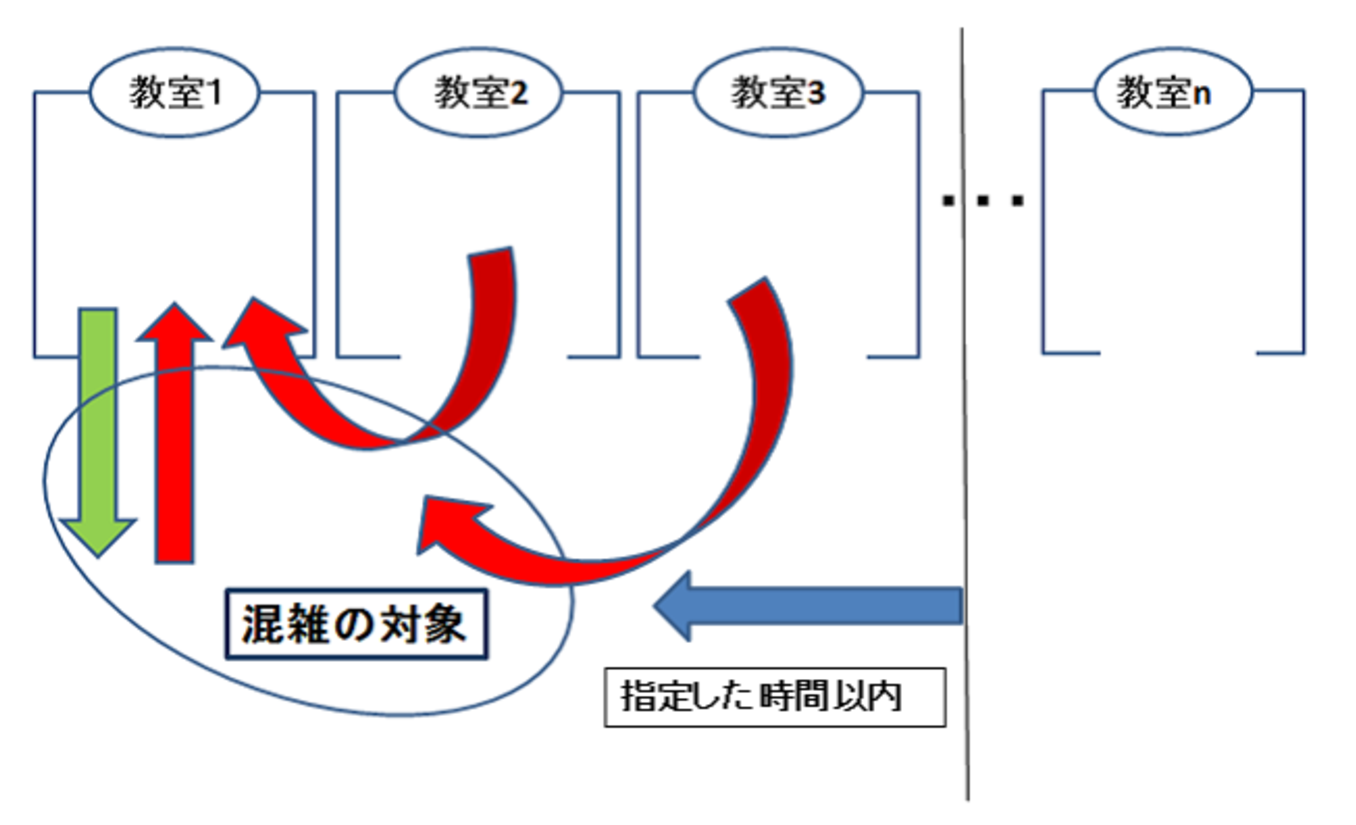
\includegraphics[clip,width=10cm]{senkounoito2.eps}
\caption{混雑の対象}
\label{senko-konzatu}
\end{center}	
\end{figure}


以下にこの制約式の左辺の項を示す.
\vspace{3.0mm}
\begin{itemize}
\item 項$(n_{j}-q_{j,j_2}\cdot d_{j,j_2})$\\

\vspace{-3.0mm}
この項は,授業$j$を$p$限に受講している人数から,$(p+1)$限に授業$j_2$を受講している学生の人数を減じることで,授業$j_2$を受講せずに退室している学生の人数を示している.
%しかし,この成分には教室を表す添字$i$が含まれていないので,授業$j$と$j_2$が開講されている対象教室が同じであるということが表現できていない.
\vspace{3.0mm}
\item 項$(q_{j_1,j_2} \cdot d_{j_1,j_2} \cdot f_{i_2,i_1})$\\

\vspace{-3.0mm}
この項は,($p+1$)限に教室$i_1$で開講される授業$j_2$を受講するために,$p$限に授業$j_1$が開講されている教室$i_2$から移動する人がいる場合,
その移動時間が混雑が起きうる移動時間を越えるなら,その移動人数は混雑の要因にならないということを示している.
混雑が起きうる移動時間とは,教室$i_1$から出て行く人や,近くの教室からの移動してくる人とは移動のタイミングが重ならないと考えられる移動時間のことである.
つまり,移動時間が一定以上かかる教室から移動してくる人は,混雑の要因とはならないと考えている.
%先行研究では,周辺いくつかの教室をこの制約の対象として考えているが,この要素では特定の1つの教室しか対象になっていない.
\vspace{3.0mm}
\item 項$ (n_{j_2} - q_{j_1,j_2}) \cdot h_{j_2}$\\

\vspace{-3.0mm}
この項は,$(p+1)$限目に教室$i_1$で開講される授業$j_2$を受講するために外から移動してくる学生数を示している.

\item 項$ (u_{i_1,j} + u_{i_1,j_2} + u_{i_2,j_1} - 2) \cdot d_{j_1,j_2} $\\

\vspace{-3.0mm}
この項は,この制約に関連する授業が同教室で連続して開講されているかを示している.
%要素(b)において,周辺の教室を指定した場合,指定した数だけ変数$u_{i,j}$を増やさなければならない.

\end{itemize}
%この式は,上記の3つの合計人数が混雑が起こると予想される人数$z$人を上回っていれば違反点数が加算されることになっている.


\vspace{3.0mm}

\item 違反点数\\
\vspace{-0.5mm}
考慮制約1, 2, 3が満たされていない場合に発生する違反点数$E_1, E_2, E_3$をそれぞれ(\ref{E_1}),(\ref{E_2}),(\ref{E_3})のように定めている:
\begin{eqnarray}
\label{E_1}
&&E_1= \sum_{j_1,j_2 \in J}\alpha_{j_1,j_2}
\end{eqnarray}
\begin{eqnarray}
\label{E_2}
&&E_2= \sum_{p \in P}\sum_{j_1 \in J1_{p}}\sum_{j_2 \in J1_{p+1}}\beta_{j_1,j_2}
\end{eqnarray}
\begin{eqnarray}
\label{E_3}
&&E_3= \sum_{p \in P}\sum_{j,j_1 \in J1_{p}}\sum_{j_2 \in J1_{p+1}}\delta_{j,j_1,j_2}
\end{eqnarray}

\vspace{5.0mm}
\item 目的関数\\
目的関数は,移動を行う全学生の移動時間の総和と,考慮制約を満たせていない場合に発生する違反点数$E_i(i=1, 2, 3)$にそれぞれの重み係数$a$と$c_i(i=1, 2, 3)$を乗じ,足し合わせた値を最小化するように定めている.
\begin{eqnarray}
&&{\rm minimize} \quad( a \cdot \sum_{i_1 \in I} \sum_{i_2 \in I} (t_{i_1,i_2} \cdot v_{i_1,i_2})) + \sum_{i=1}^{3} c_{i} \cdot E_{i} \label{eqn:mokuteki}
\end{eqnarray}
\end{itemize}

\section{使用教室と対象授業}
先行研究では,以下のデータを用いて最適化を行っている.
\begin{itemize}
\item 使用教室\\
第4学舎で使用されている一般教室である39教室を対象としている(表\ref{senkoukyousitu}).
\begin{table}[!h]
\begin{center}
\caption{先行研究で扱っている教室}
\label{senkoukyousitu}
\begin{tabular}{|c|c|c|c|c|}
\hline
1階 & 2階 & 3階 & 4階 & その他\\
\hline\hline
4-101  &   4-201A & 4-301  &  4-401  &  4-502 \\
4-102  &   4-202  & 4-302  &  4-402  &  4-3101\\
4-103  &   4-203  & 4-303  &  4-403  &  4-3201\\
4-104  &   4-204  & 4-304  &  4-404  &  4-3202\\
4-105  &   4-205  & 4-305  &  4-405  &  4-4A  \\
4-106  &   4-206  & 4-306  &  4-406  &  4-4B  \\
4-107  &   4-207  & 4-307  &  4-407  &        \\
       &   4-208  & 4-308  &  4-408  &        \\
       &   4-209  &        &         &        \\
       &   4-210  &        &         &        \\
\hline
\end{tabular}
\end{center}
\end{table}

\item 対象授業\\
理工系学部の全授業を対象としている.
しかし,OD教室などの特殊教室で開講される授業は除いている.
\end{itemize}

\section{計算環境}
先行研究では,最適化ソルバーIBM ILOG CPLEX Optimizerの分枝限定法を用いて求解を行っている.
また,表\ref{senko-kankyo}は,先行研究で用いた計算環境を示している.
\vspace{-7.0mm}
\begin{table}[H]
\begin{center}
\caption{先行研究での計算環境}
\label{senko-kankyo}
\scalebox{1.0}{ 
\begin{tabular}{cc}
\hline
OS & Microsoft Windows 7 Service Pack 1\\
CPU &Intel(R) Core(TM) i7-3930K CPU @ 3.20GHz\\ 
メモリ & 32.0 GB\\
%システム & 64ビット オぺレーティング システム\\
ソルバー1&GLPK 4.47\\
ソルバー2&IBM ILOG CPLEX 12.4.0.0\\
\hline
\end{tabular}
}
\end{center}
\end{table}


\section{実験結果}
先行研究では,まず,計算時間を制限することなく実験を行った.
しかし,約5日間に渡って計算を行い,最適解を得ることができなかった.
そのため,先行研究では,各データに対する計算時間の上限を1時間として実験を行っている.
その際,特定の教室を指定する授業は設定せず,違反係数は移動時間の最小化を優先するために$c_1=1,\, c_2=2,\, c_3=3$を与えている.

表\ref{senkou_kekka}は,先行研究での実験の結果を示している.
表\ref{senkou_kekka}より,最適解を求めることができたのは6ケースしかないということがわかる.

\if0
\begin{table}[H]
\begin{center}
\caption{先行研究での実験結果}
\label{senkou_kekka}
\scalebox{0.9}{
  \begin{tabular}{cr|ccccccccc}
\hline
最適解& \multicolumn{1}{c|}{曜限} & 制約 & 変数(0-1,整数) & nonzeros & \#1(秒) & \#2 & GAP & 計算時間(秒)\\
\hline\hline
F&春学期月曜午前 & 933306 & 4781(3320,1461) & 3649805 & 40.72 & 17248 & 100\% & 3604.03\\
F&午後 & 1156836 & 5987(4506,1481) & 4525582 & 76.05 & 58499 & 97.12\% & 3613.53 \\
F&春学期火曜午前 & 648062 & 4639(3164,1475) & 2548567 & 42.23 & 4315 & 100\% & 3603.72\\
F&午後 & 731761 & 4799(3317,1482) & 2853373 & 36.89 & 17771 & 100\% & 3605.06 \\
F&春学期水曜午前 & 595910 & 4292(2813,1479) & 2327640 & 31.37 & 9381 & 100\% & 3601.08 \\
F&午後 & 678082 & 4476(2994,1482) & 2634793 & 34.26 & 11250 & 100\% & 3600.13 \\
F&春学期木曜午前 & 192757 & 2799(1405,1394) & 744925 & 5.52 & 856 & 88.58\% & 3602.25 \\
F&午後 & 411239 & 3711(2231,1480) & 1590013 & 15.69 & 5510 & 100\% & 3600.21 \\
F&春学期金曜午前 & 200266 & 3142(1773,1369) & 772967 & 11.11 & 1379 & 13.32\% & 3604.11 \\
F&午後 & 871766 & 4981(3500,1481) & 3391847 & 43.74 & 43244 & 100\% & 3601.69 \\
T&春学期土曜午前& 36822 & 2628(1362,1266) & 133617 & 1.68 & 531 & 0.80\% & 225.23 \\
T&午後 & 48320 & 2703(1221,1482) & 171653 & 1.96 & 194 & 4.64\% & 1282.27 \\
\hline
F&秋学期月曜午前 & 706638 & 4235(2753,1482) & 2758070 & 31.90 & 9307 & 100\% & 3605.15 \\
F&午後 & 1026116 & 5861(4379,1482) & 4003702 & 75.78 & 73147 & 100\% & 3606.85 \\
F&秋学期火曜午前 & 888258 & 4922(3479,1443) & 3491939 & 51.00 & 24275 & 100\% & 3606.29 \\
F&午後 & 926884 & 4835(3353,1482) & 3606133 & 42.28 & 50741 & 100\% & 3601.60 \\
F&秋学期水曜午前 & 469738 & 3756(2312,1444) & 1832968 & 19.91 & 3295 & 100\% & 3603.42 \\
F&午後 & 723830 & 4719(3244,1475) & 2827852 & 40.08 & 7538 & 100\% & 3604.06 \\
T&秋学期木曜午前 & 80847 & 3063(1581,1482) & 306626 & 3.54 & 621 & 8.37\% & 752.94 \\
F&午後 & 815102 & 4724(3242,1482) & 3164290 & 36.33 & 11695 & 100\% & 3602.20 \\
T&秋学期金曜午前 & 77837 & 2861(1379,1482) & 296246 & 4.93 & 1733 & 0.23\% & 157.84 \\
F&午後 & 1089430 & 5587(4109,1478) & 4247281 & 61.65 & 47043 & 100\% & 3601.06 \\
T&秋学期土曜午前 & 17765 & 2647(1203,1444) & 58019 & 1.65 & 881 & 10.22\% & 17.58 \\
T&午後 & 23920 & 2561(1079,1482) & 72808 & 1.72 & 334 & 17.86\% & 164.11 \\
\hline
\multicolumn{9}{l}{※最適解の列について:最適解が求められたものは「T」,求められなかったものは「F」と表記している.}\\
\multicolumn{9}{l}{\#1 初期実行可能解が見つかる迄の時間}\\
\multicolumn{9}{l}{\#2 計算終了時の最適な目的関数の値}\\
 \end{tabular}
}
\end{center}
\end{table}
\fi

\begin{table}[H]
\begin{center}
\caption{先行研究での実験結果}
\label{senkou_kekka}
  \begin{tabular}{cr|cccc}
\hline
最適解& \multicolumn{1}{c|}{曜限} & 制約 & 変数(0-1,整数) & nonzeros & 計算時間(秒)\\
\hline\hline
F&春学期月曜午前 & 933306 & 4781(3320,1461) & 3649805 & 3604.03\\
F&午後           & 1156836& 5987(4506,1481) & 4525582 & 3613.53\\
F&火曜午前       & 648062 & 4639(3164,1475) & 2548567 & 3603.72\\
F&午後           & 731761 & 4799(3317,1482) & 2853373 & 3605.06\\
F&水曜午前       & 595910 & 4292(2813,1479) & 2327640 & 3601.08\\
F&午後           & 678082 & 4476(2994,1482) & 2634793 & 3600.13\\
F&木曜午前       & 192757 & 2799(1405,1394) & 744925  & 3602.25\\
F&午後           & 411239 & 3711(2231,1480) & 1590013 & 3600.21\\
F&金曜午前       & 200266 & 3142(1773,1369) & 772967  & 3604.11\\
F&午後           & 871766 & 4981(3500,1481) & 3391847 & 3601.69\\
T&土曜午前       & 36822  & 2628(1362,1266) & 133617  & 225.23 \\
T&午後           & 48320  & 2703(1221,1482) & 171653  & 1282.27\\
\hline
F&秋学期月曜午前 & 706638 & 4235(2753,1482) & 2758070 & 3605.15\\
F&午後           &1026116 & 5861(4379,1482) & 4003702 & 3606.85\\
F&火曜午前       & 888258 & 4922(3479,1443) & 3491939 & 3606.29\\
F&午後           & 926884 & 4835(3353,1482) & 3606133 & 3601.60\\
F&水曜午前       & 469738 & 3756(2312,1444) & 1832968 & 3603.42\\
F&午後           & 723830 & 4719(3244,1475) & 2827852 & 3604.06\\
T&木曜午前       &  80847 & 3063(1581,1482) & 306626  & 752.94 \\
F&午後           & 815102 & 4724(3242,1482) & 3164290 & 3602.20\\
T&金曜午前       &  77837 & 2861(1379,1482) & 296246  & 157.84 \\
F&午後           &1089430 & 5587(4109,1478) & 4247281 & 3601.06\\
T&土曜午前       &  17765 & 2647(1203,1444) & 58019   & 17.58  \\
T&午後           &  23920 & 2561(1079,1482) & 72808   & 164.11 \\
\hline
\multicolumn{6}{l}{※最適解の列について:最適解が求められたものは「T」,}\\
\multicolumn{6}{l}{  \hspace{39mm} 求められなかったものは「F」と表記している.}\\
 \end{tabular}
\end{center}
\end{table}


\newpage
\chapter{先行研究の問題点}
\label{mondaiten}
本研究を始めるにあたり,先行研究の検証を行った.
その結果,先行研究には以下のような問題点があることがわかった.
\begin{itemize}
\item 問題点1:考慮制約2「移動時間は指定した時間以内であることが好ましい」を表現する制約式に誤りがある.\\

\if0
\vspace{-7.0mm}
\begin{eqnarray}
&&w_{p,i_1,i_2}\cdot g_{i_1,i_2} \leq \beta_{j_1,j_2}
\label{eqn:seiyaku_first} \\ 
&& \left(\forall p \in P,\:\forall i_1 \in I,\:\forall i_2 \in I,\:\forall j_1 \in J1_p,\:\forall j_2 \in J1_{p+1}\right)\nonumber 
\end{eqnarray}
\fi

 考慮制約2を表す式(\ref{skouryo-2})においては,左辺に使われている添字が$p,\,i_1,\,i_2$であるのに対し,右辺に使われてる添字は$j_1,j_2$である.
すなわち,左辺と右辺が関連性のない式になっており,この制約式は誤りである.
\vspace{3.0mm}
\item 問題点2:変数が多い.\\
先行研究のモデルには,多くの変数が存在している.
例えば,以下の変数$w_{p,i_1,i_2}$である(再掲):
\[
\begin{array}{rcl}
w_{p,i_1,i_2} & = & \left\{ 
\begin{array}{ll}
1, & \mbox{$p$限目に教室$i_1$で授業が開講され,}\\
& \mbox{$(p+1)$限目に教室$i_2$で授業が開講されるとき}\\ 
0, & \mbox{それ以外}
\end{array}
\right.\\
\end{array}
\]
 この変数$w_{p,i_1,i_2}$は3つの添字を持つ.
すなわち,この変数$w_{p,i_1,i_2}$は,直積集合$P \times I \times I$の上で展開されるため,変数の数が非常に多くなる.
その結果,計算時間も非常に大きくなっているものと考えられる.
\vspace{3.0mm}
\item 問題点3:考慮制約3「教室内の人が入れ替わる際の混雑ができるだけ発生しないほうが好ましい」を表現する制約式の構造が非常に複雑で,計算に時間がかかっていると思われる.
また,この制約式には誤りもある.\\
\if0
\vspace{-7.0mm}
\begin{eqnarray}
&&((n_{j}-q_{j,j_2}\cdot d_{j,j_2}) + (q_{j_1,j_2} \cdot d_{j_1,j_2} \cdot f_{i_2,i_1})  \nonumber\\
&&+ (n_{j_2} - q_{j_1,j_2}) \cdot h_{j_2}) \cdot (u_{i_1,j} + u_{i_1,j_2} + u_{i_2,j_1} - 2) \cdot d_{j_1,j_2} - z \leq M \cdot \delta_{j,j_1,j_2} \\
&& \hspace{30.0mm} \left(\forall p \in P,\forall i_1 \in I,\forall i_2 \in I,\forall j \in J1_{p},\forall j_1 \in J1_{p},\forall j_2 \in J1_{p+1}\right)\nonumber \\
&& \hspace{30.0mm} \left(i_1 \neq i_2,j \neq j_1,M=十分大きな整数 \right)\nonumber
\end{eqnarray}
\fi

 考慮制約3を表す式(\ref{skouryo-3})は非常に複雑な構造になっていて,計算に非常に時間を要してしまうものと考えられる.\\

 さらに,この制約式には誤りがある.
以下にその誤りを示す.
\vspace{3.0mm}
\begin{itemize}
\item 項$(n_{j}-q_{j,j_2}\cdot d_{j,j_2})$\\

\vspace{-3.0mm}
 この項では,授業$j$を$p$限に受講している人数から,$(p+1)$限に授業$j_2$を受講している学生の人数を減じることで,
授業$j_2$を受講せずに退室している学生の人数を示そうとしている.
しかし,この成分には教室を表す添字$i$が含まれていない.
従って,授業$j$と$j_2$が開講されている教室が同じ場合,この項の対象であるということが表現できていない.
\vspace{3.0mm}
\item 項$(q_{j_1,j_2} \cdot d_{j_1,j_2} \cdot f_{i_2,i_1})$\\

\vspace{-3.0mm}
 この項では,($p+1$)限に教室$i_1$で開講される授業$j_2$を受講するために,
$p$限に授業$j_1$が開講されている教室$i_2$から移動する人がいる場合,
その移動時間が混雑の起きうる移動時間を超えるなら,その移動人数は混雑の要因にならないということを示そうとしている.
先行研究では,指定した時間以内に移動できる全ての教室から移動する学生を混雑の対象として考えている.
しかし,この項では特定の1つの教室しか対象にすることができないので,先行研究での意図とは一致していない.
\vspace{3.0mm}
\item 項$(u_{i_1,j} + u_{i_1,j_2} + u_{i_2,j_1} - 2) \cdot d_{j_1,j_2}$\\

\vspace{-3.0mm}
 この項では,この制約に関連する授業が,同じ教室で連続して開講されているかを示している.
本来考慮制約3において対象としたい移動は,図\ref{senko-konzatu}のように,指定した移動時間以内に移動できる教室を全てである.
そのような教室を対象とする場合,指定した移動時間以内に移動できる教室の数だけ変数$u_{i,j}$を増やさなければならない.
しかし,この項では,図\ref{matigai-konzatu}のように,特定の1つの教室に関してしか対応できていない.

\begin{figure}[h]
\begin{center}
		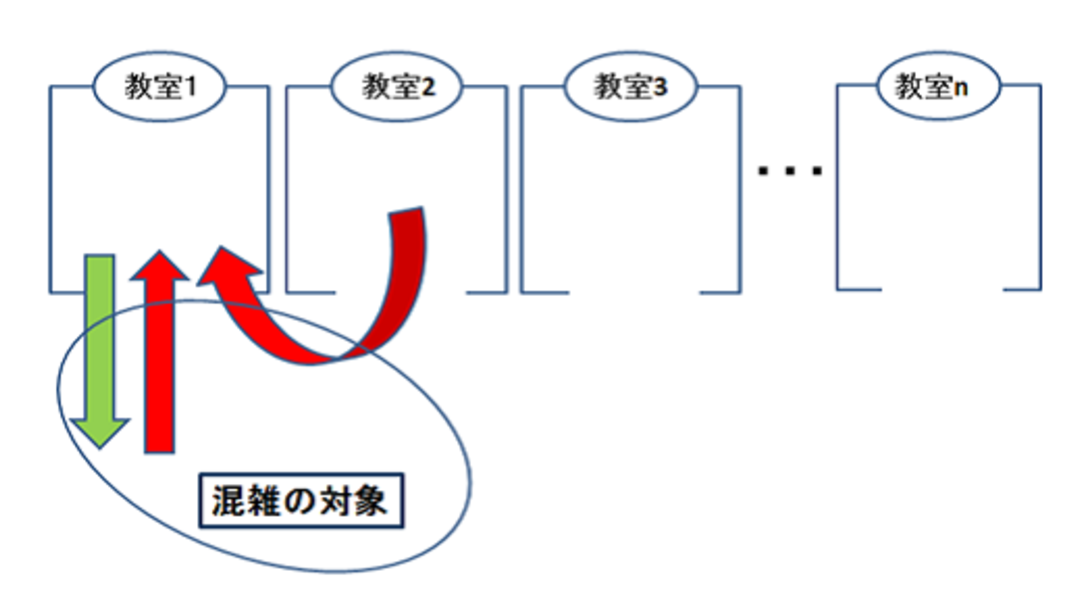
\includegraphics[clip,width=10cm]{kouryo3_old8.eps}
\caption{混雑の対象}
\label{matigai-konzatu}
\end{center}	
\end{figure}
\end{itemize}

\item 問題点4:第4学舎の全ての教室には対応できていない.\\
 先行研究で用いているデータは,表\ref{senkoukyousitu}のように,第4学舎の一般教室である39教室に対応している.
しかし,第4学舎の全ての教室には対応できていないため,データによっては実行可能解を得ることができない可能性がある.
また,OD教室のような特殊教室で開講される授業を除いていることも問題である.
\vspace{3.0mm}
\item 問題点5:授業の扱い方に誤りがある.\\
%先行研究では,全授業の「授業番号・授業名・開講学期・開講曜限・担当教員名・使用教室・履修可能学部学科・配当学部・履修者数」のデータから,授業番号で授業を扱っている.
 授業の中には,1つの授業で複数曜限に渡って開講される授業がある.
先行研究では,そのような授業も,1曜限の授業として扱っているという誤りがあった(表\ref{waruiatukai}).
また,授業の中には,複数の教員が複数の教室に分かれて開講しているものがある.
先行研究では,そのような授業も1つの教室で開講しているように扱うという誤りもあった.
そのため,使用教室数が実際よりも少なくなっている可能性がある.
また,複数の教室に分かれるはずの学生が1つの教室に集まる扱いになるので,収容人数の多い教室に授業が集中してしまう可能性もある.
さらに,特殊教室で開講される授業を計算対象から除いていることも問題である.
\begin{table}[!h]
\begin{center}
\caption{授業の扱いの例}
\label{waruiatukai}
\begin{tabular}{|c|c|c|}
\hline
授業番号 & 本来の開講曜限 & 先行研究での開講曜限 \\
\hline\hline
60247  & 金曜1,2限 & 金曜1限  \\
60272  & 火曜1限,金曜1限  & 火曜1限\\
\hline
\end{tabular}
\end{center}
\end{table}

\item 問題点6:厳密解が得られていない.\\
 先行研究では,前章で示したモデルを用いて最適化計算を行っているが,24通りのデータのうち6通りに対してしか厳密解を得ることができていない(表\ref{senkou_kekka}).
なお,厳密解を得られた6通りのうち4通りは,授業数の少ない土曜日のデータでの解であった.
\end{itemize}
\vspace{3.0mm}

\chapter{本研究における教室割当問題}

\section{先行研究からの改良点と本研究の目標}
先行研究では,移動時間の最小値を求める際,目的関数に移動時間を含め,最小化することで解を求めようとしている.
しかし,\ref{mondaiten}章で述べたように,その方法では計算に時間を要し,最適解を求めることができないケースが多くあった.
そこで本研究では,先行研究とは異なる考え方をすることでよい教室割当求めることができる方法がないかどうかを考察した.

先行研究では,全学生の移動時間の総和を最小化する教室割当を行っていた.
これに対し,本研究では,全学生の最大の移動時間を最小化することにする.
すなわち,本研究では教室割当問題を次のように定義し,これを定式化して,求解する.\\
\begin{center}
\fbox{
\begin{tabular}{c}
各授業の開講曜限が定められているとき,各休み時間における学生の\\最大の移動時間を最小化するような,授業に対する教室の割当を求めよ.
\end{tabular}
}
\end{center}
\vspace{5.0mm}

本研究では,この問題の最適解を求めるためのアプローチとして,最適化問題の中に移動時間の上限を定めるパラメータを用意する.
そして,そのパラメータを調整しながら問題を解き,実行可能解が得られるパラメータの最小値を求める.
これが,最大の移動時間の最小化となる.

なお,本研究では,最適化対象については先行研究と同様の考え方をしている.
すなわち,1日を午前・午後に分け,1週間が月曜から土曜の6日,そして1年が春・秋の2学期に分けた,合計24通りの最適化を行っている.

\if0
\section{解法}
先行研究と同様に,本研究では最大の移動時間を最小化する教室割当問題を,重み付き制約充足問題(WCSP)として扱い,また,定式化した数理計画問題を解くために,厳密解法を用いている.
\fi

\section{問題の定式化}

本研究では,以下のように教室割当問題を定式化して最適化を行っている.
制約式には先行研究からの変更点も記す.

\begin{itemize}
\item 集合と添字・パラメータ・変数
\begin{itemize}
\item 集合・添字\\

\vspace{-3.0mm}
\begin{tabular}{ll}
$p \in P$       & : 時限とその集合  \\
$p' \in P'$   & :最終時限を除いた時限とその集合  \\
$j \in J$       & : 授業とその集合  \\
$j \in JN_{p}$  &: $p$限目に開講される授業とその集合  \\
$j \in NJ$    &:一般授業とその集合  \\
$j \in SJ$     &:特殊教室を指定する授業とその集合  \\
$i \in I$        &: 教室とその集合  \\
$i \in SI$    &: 特殊教室とその集合  \\
$(i,j) \in D$   &: 特定の教室を指定する授業の組とその集合  \\
$j \in L$     &: 特別連続授業とその集合  \\
$j' \in J'$ &:教室希望のある授業とその集合  \\
$i'\in I'_{j'}$ &:授業$j'$が開講を希望する教室とその集合  \\
$pc \in PC$    &:考慮制約の番号とその集合  \\
$pa \in PA$    &:考慮制約の重みとその集合  \\
\end{tabular}
\vspace{5.0mm}
\item パラメータ\\
\vspace{-7.0mm}
\[
\begin{array}{rcl}

m_{i} & = & 
\begin{array}{ll}
 \mbox{教室$i$の定員数} 
\end{array}
\\


n_{j} & = & 
\begin{array}{ll}
 \mbox{授業$j$の受講者数} 
\end{array}
\\


t_{i_1,i_2} & = & 
\begin{array}{ll}
 \mbox{教室$i_1$と教室$i_2$間での所要移動時間} 
\end{array}
\\


q_{i_1,i_2} & = & 
\begin{array}{ll}
 \mbox{授業$i_1$と授業$i_2$の双方を受講する学生数} 
\end{array}
\\


r & = & 
\begin{array}{ll}
 \mbox{全ての移動で守る移動時間} 
\end{array}
\\


z & = & 
\begin{array}{ll}
 \mbox{混雑が起きると予測される人数} 
\end{array}
\\


d_{j_1,j_2} & = & \left\{ 
\begin{array}{ll}
	1, & \mbox{$p$限目に授業$j_1$を,$(p+1)$限目に授業$j_2$を受講する学生が存在するとき} 		\\
	0, & \mbox{それ以外}
\end{array}
\right. \\


\end{array}
\]


\vspace{5.0mm}
\item 変数\\
\[
\begin{array}{rcl}


 u_{i,j} & = & \left\{ 
\begin{array}{ll}
1, & \mbox{教室$i$に授業$j$が割り当てられているとき} \\
0, & \mbox{それ以外}
\end{array}
\right. \\


 \alpha_{j_1,j_2} & = & \left\{ 
\begin{array}{ll}
1, & \mbox{$p$限目に授業$j_1$を受講していて,$(p+1)$限目に授業$j_2$を受講せずに}\\
& \mbox{退室する学生集団と,$p$限目に授業$j_1$を受講しておらず,かつ}\\
& \mbox{$(p+1)$限目に授業$j_2$を受講するために入室する学生集団の}\\
& \mbox{合計人数が$z$人を超えて,混雑が起きる可能性が高いとき}\\
0, & \mbox{それ以外}
\end{array}
\right.
\end{array}
\]
\end{itemize}
\vspace{3.0mm}

\item 制約条件\\
\begin{itemize}
\item{絶対制約}\\
\begin{itemize}

\item {\bf  [絶対制約1] : 1つの曜限における各教室には2つ以上の授業を割り当てられない.}\\
 同じ曜限において,各教室に2つ以上の授業が割り当てられないようにするため,
教室$i$について,次の制約を与える:

\vspace{-3.0mm}
\begin{eqnarray}
\label{hzettai1} 
&&\sum_{j \in JN_{p}} u_{i,j} \leq 1 \hspace{5.0mm}
\quad \left (\forall p \in P, \: \forall i \in I \right)
\end{eqnarray} 

\vspace{5.0mm}
この制約は,先行研究の絶対制約1「1つの曜限における各教室には2つ以上の授業を割り当てられない」を改良した制約式である.
先行研究では,時限$p$時に授業$j$が割り当てられているときに1となるパラメータ$e_{p,j}$を用意している.
対して本研究では,授業$j$に時限の要素も組み込んだ$JN_p$という集合を用いることで,同じ意味の制約としている
\footnote{本研究の制約式では,授業は全て$JN_p$を用いている.これにより先行研究の$j$の集合は全て$P,JN_P$の集合となっている.}
.
\vspace{3.0mm}
\item {\bf  [絶対制約2] : 各授業には必ず1つの教室を割り当てなければならない.}\\

\vspace{-5.0mm}
 ある曜限に存在する1つの授業に対して2つ以上の教室を割り当てないようにするため,
また,1つの授業に1つも教室が割り当てられないことを防ぐため,授業$j$について,次の制約を与える:

\vspace{-3.0mm}
\begin{eqnarray}
\label{hzettai2} 
&&\sum_{i \in I} u_{i,j} = 1 \hspace{5.0mm}
\quad \left (\forall p \in P, \: \forall j \in JN_{p} \right)
\end{eqnarray} 

\vspace{5.0mm}
この制約は先行研究と同じ制約式を用いている.
\vspace{3.0mm}
\item {\bf  [絶対制約3] : 受講人数が教室の定員を超えて教室に授業を割り当ててはいけない.}\\

\vspace{-5.0mm}
 受講人数が各教室の定員を越えないようにするため,
次の制約を与える:

\vspace{-3.0mm}
\begin{eqnarray}
\label{hzettai3} 
&&\sum_{i \in I} u_{i,j}\cdot m_{i} \geq n_{j} \hspace{5.0mm}
\quad \left (\forall p \in P, \: \forall j \in JN_{p}\right)
\end{eqnarray}

\vspace{5.0mm}
この制約は先行研究と同じ制約式を用いている.
\vspace{3.0mm}
\item {\bf  [絶対制約4] : 特定の授業は指定された教室で開講されなければならない.}\\

\vspace{-5.0mm}
 本制約は,特定の設備を必要とする授業にその設備が整った指定されている教室を割り当てるための制約である.
教室$i$に授業$j$が割り当てられなければならないとき,次の制約を与える:

\vspace{-3.0mm}
\label{hzettai4} 
\begin{eqnarray}
&&u_{i,j} = 1 \hspace{5.0mm}
\quad \left(\forall (i,j) \in D\right)
\end{eqnarray}

\vspace{5.0mm}
この制約は先行研究と同じ制約式を用いている.
\vspace{3.0mm}
\item {\bf  [絶対制約4\_2] : 指定された授業でないものは特殊教室で開講されてはいけない.}\\

\vspace{-5.0mm}
 特殊教室で一般的な授業を行うことは好ましくない.
本制約は,一般的な授業に特殊教室を割り当てることを避けるための制約である.
特殊教室$i$を一般的な授業$j$に割り当ててはいけないとき,次の制約を与える:

\vspace{-3.0mm}
\begin{eqnarray}
\label{hzettai42} 
&&u_{i,j} = 0 \hspace{5.0mm}
\quad \left(\forall p \in P, \: \forall j \in JN_{p}\setminus SJ, \: \forall i \in SI\right )
\end{eqnarray}

\vspace{3.0mm}
この制約は,特殊教室,及び特殊授業を扱うために本研究において新しく追加した制約式である.

\vspace{3.0mm}
\item {\bf  [絶対制約5] : 移動時間は指定した時間以内でなければならない.}\\

\vspace{-5.0mm}
 関西大学の休み時間は10分と非常に短い.
本制約は,休み時間を移動以外のことに費やせるように,移動時間を制限するための制約である.

\vspace{-3.0mm}
\begin{eqnarray}
\label{hzettai5} 
&&u_{i_1,j_1} + u_{i_2,j_2} \leq 1\\
&&\left(\forall p \in P, \: \forall i_1 \in I,\: \forall i_2 \in I,\: \forall j_1 \in JN_{p},\: \forall j_2 \in JN_{p+1},\:t_{i1, i2} \ge r, \: d_{j1, j2} = 1\right)\nonumber
\end{eqnarray}

\vspace{3.0mm}
この制約は,先行研究の考慮制約2「移動時間は指定した時間以内であることが好ましい」を改良したものである.
先行研究では,一定以上の休み時間を確保できない学生が存在する可能性がある.
本研究では,この制約を絶対制約にすることで全学生の移動時間を一定以下に制限し,全学生に一定時間以上の休み時間を確保している.

 この改良により,前章の問題点1『考慮制約2「移動時間は指定した時間以内であることが好ましい」の制約式に誤りがある』を解消している.
またこの制約式は,3つの添字を持つ変数$w_{p,i_1,i_2}$を用いず,他の制約式でも用いているパラメータ$d_{j_1,j_2}$を用いている.
さらに,2つの添字を持つ変数$\beta_{j_1,j_2}$も用いていない.
これらのことより,前章の問題点2「変数が多い」も解消している.

\vspace{3.0mm}
\item {\bf  [絶対制約6] : 特別連続授業は同じ教室で開講されなければならない.}\\

\vspace{-5.0mm}
 特別連続授業(授業内容が同一,または非常に関連性の高い2限以上連続で開講される授業)は双方を受講している学生が多い.
従って,特別連続授業同一の教室で開講されるべきである.
本制約は,特別連続授業を同一教室で行うための制約である.

\vspace{-3.0mm}
\begin{eqnarray}
\label{hzettai6} 
&&u_{i_1,j_1}= u_{i_2,j_2} \quad \left(i \in I ,\: (j_1, j_2) \in L \right)
\end{eqnarray}

\vspace{3.0mm}
この制約は,先行研究の考慮制約1「特別連続授業は同じ教室で開講されることが好ましい」を改良したものである.
本研究では,この制約を絶対制約にすることで,大勢の学生が移動する可能性を低くしている.
また,この制約は,先行研究の考慮制約1「特別連続授業は同じ教室で開講されることが好ましい」で用いられている変数$\alpha_{j_1,j_2}$を用いずに定式化している.
従って,これは前章の問題点2「変数が多い」を解消している.
\end{itemize}

\vspace{5.0mm}
\item 考慮制約\\
\vspace{-5.0mm}
\begin{itemize}
\item {\bf  [考慮制約1] : 教室内の人が入れ替わる際の混雑ができるだけ発生しないほうが好ましい.}\\

\vspace{-5.0mm}
 昼休みを除く各時限間の教室では,移動して教室に入ってくる学生と,授業が終わって教室から出て行く学生によって混雑が起きる可能性がある.
しかし,混雑は移動時間の増加につながるため,できるだけ避けたいことである.
本制約は,授業間移動によって発生する混雑による移動時間の増加を,できるだけ避けるための制約である.\\

\vspace{-10.0mm}
\begin{eqnarray}
\label{hkouryo1} 
&&\left(u_{i,j_1} + u_{i,j_2} - 1\right) \le \alpha_{j_1, j_2}  \\
&&(\forall p' \in P', \: \forall j_1 \in JN_{p'}, \: \forall j_2 \in JN_{p'+1} ,\nonumber \\
&&\hspace{30mm} (n_{j_1} - q_{j_1, j_2}) + (n_{j_2} - q_{j_1, j_2})) - z > 0, \: d_{j_1, j_2} = 1)\nonumber 
%&&\left(\forall p' \in P', \: \forall j_1 \in JN_{p'}, \: \forall j_2 \in JN_{p'+1} \right)\nonumber \\
%&&\left((n_{j_1} - q_{j_1, j_2}) + (n_{j_2} - q_{j_1, j_2})) - z > 0, \: d_{j_1, j_2} = 1\right)\nonumber 
\end{eqnarray}

\begin{eqnarray}
\label{hkouryo12} 
&&k_1= \sum_{p' \in P'} \sum_{j_1 \in JN_{p'}} \sum_{j_2\_ \in JN_{p'}} \alpha_{j_1, j_2}
\end{eqnarray}

\vspace{3.0mm}
この制約は,先行研究の考慮制約3「教室内の人が入れ替わる際の混雑ができるだけ発生しないほうが好ましい」を改良した制約である.
混雑のタイミングは,対象教室の授業が延長されたり,遠くの教室の授業が早く終了するなど,様々な要因があるため,予測することは非常に難しい.
そのため,本研究では,図\ref{hkonzatu}のように,混雑の原因となる人数は,対象教室を出入りする全ての学生の合計としている.

 (\ref{hkouryo1}),(\ref{hkouryo12})では,移動人数が混雑が発生すると考えられる人数である$z$人を越えると,条件を違反した指標$\alpha_{j_1, j_2}$が1となり,その合計が違反点数$k_1$となる.

\begin{figure}[h]
\begin{center}
		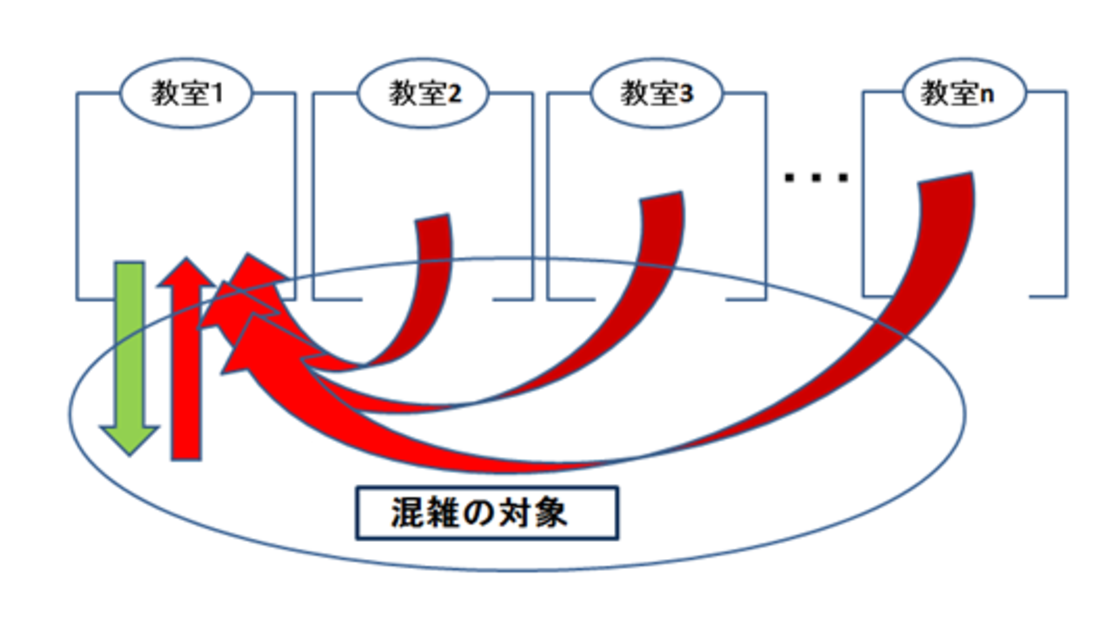
\includegraphics[clip,width=10cm]{kouryo3_new8.eps}
\caption{本研究における混雑の対象}
\label{hkonzatu}
\end{center}	
\end{figure}

 この考え方より,この制約は「対象教室で起こり得る最大の混雑を抑える」ということを示している.
この改良によって,制約式の構造を簡素化することができ,
前章の問題点3『考慮制約3「教室内の人が入れ替わる際の混雑ができるだけ発生しないほうが好ましい」の構造が非常に複雑で,計算に時間がかかっている.また,この制約式に誤りがある』を解消している.
また,この制約式は3つの添字を持つ変数$\delta_{j,\;j_1,\;j_2}$から,2つの添字を持つ変数$\alpha_{j_1,j_2}$に変更している.
これにより,前章の問題点2「変数が多い」を解消していることがわかる.
この変更により,計算時間を短縮できることが期待できる.
\vspace{5.0mm}
\item {\bf  [考慮制約2] : 希望教室があれば,その教室で授業を開講したい.}\\

\vspace{-5.0mm}
 学生や教員には,何らかの理由(研究室が近いなど)で授業を開講してほしい教室があると思われる.
本制約は,できるだけ希望した教室で授業を開講するための制約である.

\vspace{-3.0mm}
\begin{eqnarray}
\label{hkouryo2} 
&&k_2= \sum_{j' \in J'}  \sum_{i' \in I'_{j'}}u_{i', j'}
\end{eqnarray}

\vspace{5.0mm}
この制約は,希望教室で授業を開講するために,本研究で新しく追加した制約である.
本制約では,ひとつの授業で複数の教室を希望することができる.
しかし,同じ曜限で同じ教室を希望する授業が複数あった場合や,ひとつの授業で複数の希望教室がある場合,
または教室希望を叶えると他の教室の割当が不可能になってしまう場合,絶対制約を満たすことができず,解を求められない.
本制約はそのような場合に対応するため,考慮制約となっている.

\vspace{5.0mm}
\end{itemize}
\end{itemize}
\item 目的関数\\
目的関数は,考慮制約1を満たせていない場合に発生する違反指標の合計$k_1$と,
考慮制約2を満たせた場合の指標の合計$k_2$に,それぞれ重み$pa_1$,$pa_2$を乗じたものの合計値を最小化するように定める.
ただし,$k_2$については制約を満たした場合に指標が発生するので,重み$pa_2$は必ず負の値でなければならない.
\begin{eqnarray}
\label{hmokuteki} 
&&{\rm minimize} \quad \sum_{pc \in PC} (pa_{pc} \cdot k_{pc}) \label{eqn:mokuteki}
\end{eqnarray}

本問題では,全学生の移動時間に上限を設けている.
そのため,各学生の移動時間の総和を最小化する事は行わない.
その結果,本問題では目的関数に$v_{i_1,i_2}$を含んでいない.
これにより,前章の問題点2「変数が多い」を解消している.
\end{itemize}

この問題を解くことは,学生全員が$r$秒以下で移動できるような教室割当問題を解くということと同意である.
$r$を変化させることで,学生の最大の移動時間が変化する.
従って,$r$を小さくしていくことで,学生の最大の移動時間の最小値を求めることができる.
本研究では,この解を求めることが,教室割当問題の解を求めることであると考えている.

\section{使用教室と対象授業}
本研究では以下のデータを使って最適化を行っている.
\begin{itemize}
\item 使用教室\\
 本研究では,第4学舎の一般教室である44教室(表\ref{hkyousitu})と,OD教室などの特殊教室である23教室(表\ref{tokushu})の合計67教室を計算対象としている.
これより,前章の問題点4「第4学舎の全ての教室に対応できていない」を解消し,第4学舎で開講される全ての授業に対応することができている.\\
 なお,本研究で扱っている特殊教室を付録\ref{hurokupara}の表\ref{tokushu}に示す.
また,教室間の移動時間であるパラメータ$t_{i_1,i_2}$は,表\ref{paramt}のように定めている.


\begin{table}[!h]
\begin{center}
\caption{本研究で扱っている一般教室}
\label{hkyousitu}
\begin{tabular}{|c|c|c|c|c|}
\hline
1階 & 2階 & 3階 & 4階 & その他\\
\hline\hline
\ 4-101  & \ 4-201A & \ 4-301  &  \ 4-401  & *4-501  \\
\ 4-102  & *4-201B  & \ 4-302  &  \ 4-402  &\ 4-502  \\
\ 4-103  & \ 4-202  & \ 4-303  &  \ 4-403  &\ 4-3101 \\
\ 4-104  & \ 4-203  & \ 4-304  &  \ 4-404  &\ 4-3201 \\
\ 4-105  & \ 4-204  & \ 4-305  &  \ 4-405  &\ 4-3202 \\
\ 4-106  & \ 4-205  & \ 4-306  &  \ 4-406  & *4-3401 \\
\ 4-107  & \ 4-206  & \ 4-307  &  \ 4-407  & *4-3402 \\
         & \ 4-207  & \ 4-308  &  \ 4-408  & *4-3403 \\
         & \ 4-208  &          &           &\ 4-4A   \\
         & \ 4-209  &          &           &\ 4-4B   \\
         & \ 4-210  &          &           &         \\
\hline
\multicolumn{5}{l}{*:本研究で追加した教室}\\
\end{tabular}
\end{center}
\end{table}


\item 対象授業\\
 理工系学部で開講される全授業を授業番号によって扱っている.
また,本研究では,特殊教室で行われる授業も同様に扱っている.

 授業の中には,1つの授業であるにも関わらず,複数の曜限で開講しているものがある.
本研究では,{\bf 各授業の授業番号に学期・曜限の情報を付加させ,授業を分割する}ことで,このような授業に対応している.
さらに,複数の教員が複数の教室を使用して開講している授業が存在している.
しかし,この授業は,絶対制約1「1つの曜限における各教室には2つ以上の授業を割り当てられない」を守ることができない.
そこで,本研究では,{\bf 「複数の教員が担当し,かつ複数の教室を扱っているとき,教員と教室の少ない方の数だけ授業を分割する」}ということを行っている.
これにより,本研究では,ひとつの授業を「授業番号\_学期・曜限\_分割番号」と表示している.
それぞれの要素は,表\ref{jugyou}のように構成される.

\vspace{-3mm}

\begin{table}[H]
\caption{授業の扱い方}
\label{jugyou}
\begin{center}
\begin{tabular}{rl}
\hline
授業番号 & 授業に割り当てられている番号\\
\hline
学期 & o:春学期に開講\\
 & x:秋学期に開講\\
\hline
曜日 & 月曜から土曜までそれぞれ「Mo,Tu,We,Th,Fr,Sa」\\
\hline
時限 & 開講される時限\\
\hline
分割番号 & 授業を分割した時,分割したことを示すための番号\\
\hline
\end{tabular}
\end{center}
\end{table}

\vspace{-10mm}
分割番号は,分割した分だけ数値が示している.
例えば,3つに分割されてる授業は,分割番号が1, 2, 3となっている授業がそれぞれ存在しているということである.
その際,履修人数,及び移動人数は分割した数だけ等分されている.
以下に授業の例を示す.\\
\vspace{-5mm}
\begin{itemize}
\item 授業番号00561(春学期の月曜2限に開講,担当教員1人,使用教室1つ)\\
これは,最も一般的な授業の形式である.
「{\bf 00561\_oMo2\_1}」と示す.
\item 授業番号65392(春学期の月曜3, 4, 5限に開講,担当教員1人,使用教室1つ)\\
この授業は連続授業である.
3, 4, 5限にそれぞれ対応すると,「{\bf 65392\_oMo3\_1, 65392\_oMo4\_1, 65392\_oMo5\_1}」となる.
\item 授業番号65180(春学期の月曜2限に開講,担当教員2人,使用教室2つ)\\
この授業は複数の教員が担当し,複数の教室を使って開講している.
この授業の場合,教員と教室の数が共に2つなので,授業は2つに分割される.
よって,この授業は,「{\bf 65180\_oMo2\_1, 65180\_oMo2\_2}」となる.
\item 授業番号60273(春学期の火曜1限,金曜1限に開講,担当教員1人,使用教室1つ)\\
この授業は,複数の曜限で開講されている.
それぞれの曜限に対応すると,\\
「{\bf 60273\_oTu1\_1, 60273\_oFr1\_1}」となる.
\item 授業番号65186(春学期の月曜3限,金曜2限に開講,担当教員3人,使用教室3つ)\\
まず,この授業は複数の教員と複数の教室がある.
この授業の場合,教員と教室の数が共に3つなので,授業は3つに分割される.
また,複数の曜限で開講されているので,それぞれに対応すると,「{\bf 62227\_oMo3\_1, 62227\_oMo3\_2, 62227\_oMo3\_3, 62227\_oFr2\_1, 62227\_oFr2\_2, 62227\_oFr2\_3}」となる.
\end{itemize}
\vspace{3.0mm}
この処理により,前章の問題点5「授業の取り扱いに誤りがある」を解消している.

 表\ref{k:normal_information}に,本研究で扱う各曜限の授業数を示す.
\begin{table}[H]
\caption{各学期曜限の授業数}
\label{k:normal_information}
\begin{center}
\begin{tabular}{c|cc|ccc|cc|ccc}
\hline
 & \multicolumn{2}{|c}{春学期午前} &\multicolumn{3}{|c}{春学期午後} &\multicolumn{2}{|c}{秋学期午前} &\multicolumn{3}{|c}{秋学期午後} \\
\hline
曜日 & 1限 & 2限 & 3限 & 4限 & 5限 &  1限 & 2限 & 3限 & 4限 & 5限\\
\hline
月曜  & 21  & 36  & 45 & 32  & 25  & 24  & 30 & 38  & 33 & 18 \\
火曜  & 35  & 39  & 33 & 34  & 24  & 25  & 37 & 35  & 31 & 20 \\
水曜  & 22  & 34  & 34 & 26  & 14  & 24  & 32 & 36  & 28 & 13 \\
木曜  & 20  & 23  & 21 & 25  & 24  & 17  & 34 & 36  & 29 & 24 \\
金曜  & 25  & 35  & 39 & 38  & 21  & 18  & 35 & 44  & 33 & 21 \\
土曜  & 11  & 18  & 16 & 11  & 5   & 12  & 19 & 16  & 13 & 4  \\
\hline
\end{tabular}
\end{center}
\end{table}





\end{itemize}



\if0
\documentclass[12pt, a4paper, fleqn]{jreport}

\usepackage{graduatethesis}
\usepackage{listings,jlisting}
\usepackage{cite}
\usepackage{here}


\begin{document}
\setcounter{tocdepth}{2}
\setlength{\mathindent}{0zw}
\pagenumbering{roman}
\pagenumbering{arabic}
\setcounter{totalnumber}{3}
\setcounter{topnumber}{3}
\renewcommand{\topfraction}{0.99}
\renewcommand{\bottomfraction}{0.99}
\renewcommand{\textfraction}{0.0}

\lstset{
  basicstyle={\ttfamily},
  breaklines=true,
  columns=[l]{fullflexible},
  lineskip=-0.5zw,
}

\setlength{\textwidth}{\paperwidth}   %%本文を用紙の横サイズにする
\addtolength{\textwidth}{-2in}         %それを2インチ引く
\setlength{\textheight}{\paperheight} %%本文を用紙の縦サイズにする
\addtolength{\textheight}{-2in}        %それを2インチ引く
\setlength{\topmargin}{0pt}            %ページ上端の余白を消す
\addtolength{\topmargin}{-\headheight} %(ページ上端の余白)-(ヘッダーの高さ)
\addtolength{\topmargin}{-\headsep}    %                  -(ヘッダーと本文の余白)
\setlength{\oddsidemargin}{0pt}       %%奇数(右)ページの左余白消す
\setlength{\evensidemargin}{0pt}      %%偶数(左)ページの左余白を消す


\fi



\chapter{数値実験}
本章では,本研究で作成した数理計画モデルと,実際に使用している関西大学の理工系全学部の時間割を用いて,様々な教室割当を行った実験内容と結果について述べる.

本研究では,以下の実験を行った.
\begin{itemize}
\item 予備実験1: サンプルデータを用いた,各制約式が正しく機能するかを確かめる実験
\item 予備実験2:春学期火曜午前のデータを用いた,移動時間の制限を300秒とする確認実験
\item 本実験1:移動時間の制限を小さくしていき,最大移動時間の最小値を求める実験
\item 本実験2:本実験1において最大移動時間が大きいデータから原因の授業を取り除いた実験
\item 本実験3:考慮制約2の希望教室を設定した春学期火曜午前のデータを用いた実験
\end{itemize}

なお,本研究では,全ての実験においてパラメータ$pa_1 = 1$,$pa_2 = -1$,$z = 100$を与えている.
\section{計算環境}
本研究では,先行研究と同様に,最適化ソルバーIBM ILOG CPLEXの分枝限定法を用いて求解を行っている.
表\ref{kankyo}は,本研究で用いた計算環境を示している.

\begin{table}[H]
\begin{center}
\label{kankyo}
\caption{計算環境}
\scalebox{1.0}{ 
\begin{tabular}{cc}
\hline
OS & Microsoft Windows 7 Home Premium Service Pack 1\\
CPU &Intel(R) Core(TM) i5-2520M CPU @ 2.50GHz\\ 
メモリ & 8.0 GB\\
ソルバー1&GLPK 4.47\\
ソルバー2&IBM ILOG CPLEX 12.5.0.0\\
\hline
\end{tabular}
}
\end{center}
\end{table}
\section{予備実験}
\subsection{予備実験1:各制約式が正しいく機能するかを確かめる実験}
予備実験1は,ごく小さな規模のサンプルデータを用いた数値計算である.
予備実験1の目的は,モデルファイルが意図した形で展開され,制約を満たす解が得られるかどうかを確かめることである.

表\ref{b:normal_information}~表\ref{f:normal_information}は,使用したサンプルデータの内容を示している.\\

\begin{table}[H]
\caption{サンプルデータ:教室毎の定員}
\label{b:normal_information}
\begin{center}
\begin{tabular}{c|ccccccc}
\hline
教室 & 101 & 102 & 103 & 104 & 105 & 106 & 107 \\
定員 & 150 & 150 & 180 & 100 & 180 & 180 & 100  \\
\hline
\end{tabular}
\end{center}
\end{table}

\begin{table}[H]
\caption{サンプルデータ:授業と受講者数}
\label{c:normal_information}
\begin{center}
\begin{tabular}{c|cccc|cccccc}
\hline
開講時限 & \multicolumn{4}{c|}{1} & \multicolumn{6}{c}{2} \\
\hline
授業 & 1001& 1002 & 1003 & 1004 & 1005 & 1006 & 1007 & 1008 & 1009 & 1010 \\
受講者 & 150 & 40 & 80 & 120 & 150 & 150 & 80 & 120 & 100 & 80  \\
\hline
\end{tabular}
\end{center}
\end{table}

\begin{table}[H]
\caption{サンプルデータ:パラメータ$q_{i_1,i_2}$}
\label{d:normal_information}
\begin{center}
\begin{tabular}{c|cc}
\hline
 移動前の授業 & 移動先の授業 & 移動する人数 \\
\hline\hline
     & 1005 & 20 \\
1001 & 1006 & 10 \\
     & 1007 & 30 \\
\hline
     & 1005 & 10 \\
1002 & 1006 & 10 \\
     & 1007 & 20 \\
\hline
1003 & 1005 & 30 \\
     & 1006 & 30 \\
\hline
1004 & 1008 & 120 \\
\hline
 \multicolumn{3}{l}{※値が0であるものは省略している}
\end{tabular}
\end{center}
\end{table}

\begin{table}[H]
\caption{サンプルデータ:教室間の移動時間(秒)}
\label{e:normal_information}
\begin{center}
\begin{tabular}{c|ccccccc}
\hline
教室 & 101 & 102 & 103 & 104 & 105 & 106 & 107 \\
\hline\hline
 101 & 0   &  15 &   30 &   45  & 75  &  90 &  105 \\
 102 & 15  &  0  &   15 &   30  & 60  &  75 &  90  \\
 103 & 30  &  15 &   0  &   15  & 45  &  60 &  75  \\
 104 & 45  &  30 &   15 &   0   & 30  &  45 &  60  \\
 105 & 75  &  60 &   45 &   30  & 0   &  15 &  30  \\
 106 & 90  &  75 &   60 &   45  & 15  &  0  &  15  \\	
 107 & 105 &  90 &   75 &   60  & 30  &  15 &  0   \\
\hline
\end{tabular}
\end{center}
\end{table}

\begin{table}[H]
\caption{サンプルデータ:その他の設定}
\label{f:normal_information}
\begin{center}
\begin{tabular}{c|c}
\hline
教室指定 & (101,1001),(101,1005),(107,1010) \\
特別連続授業 & (1004,1008)\\
希望教室 & (101,1002),(102,1002)\\
& (105,1003),(106,1003)\\
\hline
\end{tabular}
\end{center}
\end{table}

ここでは,以下の2つの実験を行った.
\begin{itemize}
\item{予備実験1-1}\\
教室$103$を特殊教室に指定して実験を行った.
この実験では,教室$103$に授業は割り当てられない設定になっている.

\item{予備実験1-2}\\
教室$107$を特殊教室に指定して実験を行った.
この実験では,教室$103$にも授業が割り当てられる設定になっている.

\end{itemize}

予備実験1では,移動時間の上限$r$を70秒から5秒ごとに小さくしながら実験を行った.
表\ref{g:normal_information},表\ref{h:normal_information}に,予備実験1の結果を示す.

\begin{table}[H]
\caption{予備実験1-1の結果}
\label{g:normal_information}
\begin{center}
\begin{tabular}{|c|c||cccc|cccccc|}
\hline
移動時間& & \multicolumn{4}{|c|}{1限} &  \multicolumn{6}{|c|}{2限} \\
\hline
70 & 授業 & 1001 & 1002 & 1003 & 1004 & 1005 & 1006 & 1007 & 1009 & 1008 & 1010 \\ 
& 教室 & 101 & 102 & 105 & 106 & 101 & 102 & 104 & 105 & 106 & 107  \\ \cline{2-11}
\hline
65 & 授業 & 1001 & 1002 & 1003 & 1004 & 1005 & 1006 & 1007 & 1009 & 1008 & 1010 \\ 
& 教室 & 101 & 102 & 105 & 106 & 101 & 102 & 104 & 105 & 106 & 107  \\ \cline{2-11}
\hline
60 & 授業 & 1001 & 1003 & 1002 & 1004 & 1005 & 1006 & 1007 & 1009 & 1008 & 1010 \\ 
& 教室 & 101 & 102 & 104 & 106 & 101 & 102 & 104 & 105 & 106 & 107  \\ \cline{2-11}
\hline
55 & 授業 & 1001 & 1003 & 1002 & 1004 & 1005 & 1006 & 1007 & 1009 & 1008 & 1010 \\
& 教室 & 101 & 102 & 104 & 106 & 101 & 102 & 104 & 105 & 106 & 107  \\\cline{2-11}
\hline
50 & 授業 & 1001 & 1003 & 1002 & 1004 & 1005 & 1006 & 1007 & 1009 & 1008 & 1010 \\ 
& 教室 & 101 & 102 & 104 & 106 & 101 & 102 & 104 & 105 & 106 & 107  \\ \cline{2-11}
\hline
45~  &  \multicolumn{11}{|c|}{最適解求解不可}\\
\hline
\end{tabular}
\end{center}
\end{table}

\begin{table}[H]
\caption{予備実験1-2の結果}
\label{h:normal_information}
\begin{center}
\begin{tabular}{|c|c||cccc|cccccc|}
\hline
移動時間& & \multicolumn{4}{|c|}{1限} &  \multicolumn{6}{|c|}{2限} \\
\hline
70 & 授業 & 1001 & 1002 & 1004 & 1003 & 1005 & 1006 & 1007 & 1008 & 1009 & 1010 \\
& 教室 & 101 & 102 & 105 & 106 & 101 & 103 & 104 & 105 & 106 & 107 \\ \cline{2-11}
\hline
65 & 授業 & 1001 & 1002 & 1004 & 1003 & 1005 & 1006 & 1007 & 1008 & 1009 & 1010 \\
& 教室 & 101 & 102 & 105 & 106 & 101 & 103 & 104 & 105 & 106 & 107 \\\cline{2-11}
\hline
60 & 授業 & 1001 & 1002 & 1003 & 1004 & 1005 & 1009 & 1006 & 1007 & 1008 & 1010 \\
& 教室 & 101 & 102 & 105 & 106 & 101 & 102 & 103 & 104 & 106 & 107 \\ \cline{2-11}
\hline
55 & 授業 & 1001 & 1002 & 1003 & 1004 & 1005 & 1009 & 1006 & 1007 & 1008 & 1010 \\
& 教室 & 101 & 102 & 105 & 106 & 101 & 102 & 103 & 104 & 106 & 107 \\ \cline{2-11}
\hline
50 & 授業 & 1001 & 1002 & 1003 & 1004 & 1005 & 1009 & 1006 & 1007 & 1008 & 1010 \\
& 教室 & 101 & 102 & 105 & 106 & 101 & 102 & 103 & 104 & 106 & 107 \\ \cline{2-11}
\hline
45~  &  \multicolumn{11}{|c|}{最適解求解不可}\\
\hline
\end{tabular}
\end{center}
\end{table}

表\ref{g:normal_information},表\ref{h:normal_information}より,教室$103$を特殊教室としている予備実験1-1では教室$103$に授業を割り当てず,教室$103$を一般教室とした予備実験1-2では,教室$103$に授業を割り当てていることがわかる.
また,どちらの実験も移動時間の制限が45秒のとき,実行可能解を得られなくなった.
従って,どちらの実験も移動時間50秒が最小の最大移動時間であることがわかる.
これらより,どちらの実験も全ての制約が満たされていて,意図した動きをしていることがわかる.


\subsection{予備実験2:実データに対する求解時間の確認実験}
予備実験2は,春学期火曜午前のデータを用いた数値実験である.
予備実験2の目的は,以下の3つである.
\begin{itemize}
\item{データファイル変換のプログラムが意図した形で動いているか確かめる}
\item{大規模の問題を解く際に本モデルでバグが発生しないかどうかを確かめる}
\item{最適解を求める際,具体的にどれほどの時間を要するのかを確かめる}
\end{itemize}

以上のことを調べるために,本研究では2つの実験を行った.

\begin{itemize}
\item{予備実験2-1}\\
全ての制約を考慮に入れた状態で数値実験を行った.
なお,3つの授業に,希望教室として同じ2教室を指定している.
\item{予備実験2-2}\\
希望教室の指定の有無で,求解に要する時間の差を調べるため,希望教室をのぞいて数値実験を行った.
\end{itemize}

なお,春学期月曜午前のデータには,特殊教室で行わなければならない授業,及び教室指定を行う授業が存在していなかったため,予備実験2では春学期火曜午前のデータを用いて実験を行っている.
また,予備実験2ではどちらも移動時間の制限を300秒として実験を行っている.

予備実験2を行った結果,どちらの実験でも全ての制約を満たしていることがわかった.
また,計算時間は,予備実験2-1が0.20秒,予備実験2-2が0.16秒と,実データを用いても短い計算時間で求解できることがわかった.
そのため,午前よりもデータ量の大きい午後のデータを用いても,膨大な計算時間にはならないと考えられる.
また,希望教室の設定によって,計算時間が長くなることはない,ということが確認できた.






本研究では,この結果を受け,次節に本実験においても時間を制限することなく計算を行うことにした.
また,本実験においては,希望教室を用意せずに最適化を行っている.

\section{本実験}
本節では,前節で行った予備実験の結果を基に行った数値実験について説明する.

\subsection{本実験1:最大移動時間の最小値を求める実験}
本実験1は,全実データ(24種類に分かれたデータ)を用いて,各データにおける最大の移動時間の最小値を求める実験である.
本実験1の実験順序を説明する.
\begin{enumerate}
\item 各データにおける移動時間を制限するパラメータ$r$を300秒から0秒まで,10秒ごとに小さくして最適化を行う.
\item (1)において,最適解を得たケースのうち,最もパラメータ$r$の小さい値から,さらに1秒ごとに小さくして最適化を行う.
\end{enumerate}
これにより,各データにおける最大の移動時間の最小値を求めることができる.


\if0
\begin{table}[H]
\caption{本実験1の最大移動時間の最小値(秒)}
\label{j:normal_information}
\begin{center}
\begin{tabular}{c|c|c|c|c}
\hline
曜日 & 春学期午前 & 春学期午後 & 秋学期午前 & 秋学期午後\\
\hline
月曜  & 96  & 251 & 50 & 67 \\
火曜  & 76  & 141 & 68 & 49 \\
水曜  & 58  & 52  & 57 & 123\\
木曜  & 34  & 251 & 58 & 60 \\
金曜  & 103 & 74  & 89 & 80 \\
土曜  & 33  & 27  & 34 & 74 \\
\hline
\end{tabular}
\end{center}
\end{table}
\fi

\begin{table}[H]
\begin{center}
\caption{本実験1の結果}
\label{j:normal_information}
\begin{tabular}{|r|cccccc|}
\hline
 \multicolumn{1}{|c|}{曜限} &  最大(秒)  & 平均(秒) & 制約 & 変数 & nonzeros & *計算時間(秒)\\
\hline
春学期月曜午前  & 96  & 58.3 & 2569 & 1854 & 26538 &  4.34\\  
午後            & 251 & 53.6 & 3383 & 2929 & 19953 &  0.44\\
火曜午前        & 76  & 39.4 & 1753 & 2150 & 28679 &  1.04\\
午後            & 141 & 53.8 & 2321 & 2420 & 21858 &  0.65\\
水曜午前        & 58  & 28.4 & 1301 & 1422 & 19247 &  2.25\\
午後            & 52  & 18.0 & 2303 & 1843 & 45593 & 19.41\\
木曜午前        & 34  & 14.1 & 1054 & 930  & 16759 &  1.53\\
午後            & 251 & 37.3 & 1239 & 1520 & 8582  &  0.17\\
金曜午前        & 103 & 47.5 & 2059 & 1524 & 18978 &  0.89\\
午後            & 74  & 20.9 & 1991 & 2174 & 26723 &  2.01\\
土曜午前        & 33  & 12.6 & 515  & 1131 & 9352  &  0.27\\
午後            & 27  & 7.3  & 474  & 898  & 11303 &  1.40\\
\hline                                        	         
秋学期月曜午前  & 50  & 22.4 & 2614 & 1844 & 45661 & 80.62\\
午後            & 67  & 27.3 & 1327 & 1877 & 18494 &  3.29\\          
火曜午前        & 68  & 32.9 & 1945 & 1600 & 24354 &  1.42\\
午後            & 49  & 12.5 & 2005 & 1822 & 32710 & 42.46\\          
水曜午前        & 57  & 30.2 & 2571 & 1623 & 33821 &  2.12\\
午後            & 123 & 43.1 & 1904 & 2234 & 17342 &  0.56\\          
木曜午前        & 58  & 39.4 & 2236 & 1402 & 28246 & 20.69\\
午後            & 60  & 21.7 & 2548 & 2099 & 44146 & 60.58\\          
金曜午前        & 89  & 45.9 & 1003 & 1396 & 12369 &  0.56\\
午後            & 80  & 28.4 & 2571 & 2396 & 29883 &  2.96\\          
土曜午前        & 34  & 19.7 & 168  & 668  & 1672  &  0.30\\
午後            & 74  & 52.7 & 481  & 1199 & 11385 &  0.13\\
\hline
\multicolumn{7}{l}{※本定式化において,変数は全て$0\_1$変数である}\\
\multicolumn{7}{l}{*:最大の移動時間の最小値を移動時間の上限としている時の計算時間}\\
\end{tabular}
\end{center}
\end{table}

\begin{figure}[thpb]
 \begin{center}
 \hspace{5mm} 
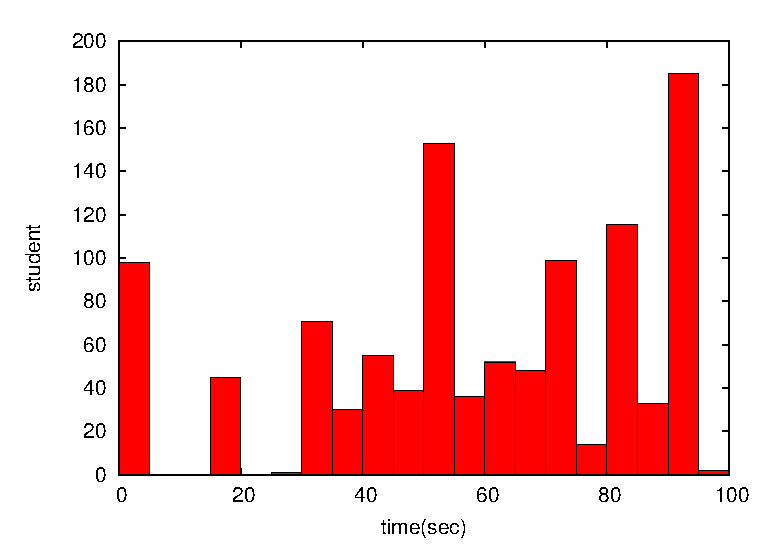
\includegraphics[bb=0 0 390 248,clip,scale=1.0]{oMo12_hist.eps}
 \hspace{-10mm} 
\vspace{-5mm}
  \caption{移動時間ごとの学生数(春学期月曜午前)}
  \label{omo12}
 \end{center}
\end{figure}

表\ref{j:normal_information}は,本実験1での実験結果である.
表\ref{j:normal_information}より,本実験1では,全ての曜限において,比較的短い計算時間で最大の移動時間の最小値を求めることができた.
また,先行研究の結果(表\ref{senkou_kekka})と比べて,制約数は遥かに小さくなっていることがわかる.
さらに,変数についても,全ての曜限において,最低でも半分以下になっている.
これらの要因によって,本実験1では,短い計算時間で解を得ることができたと考えられる.

図\ref{omo12}は,春学期月曜午前における,移動時間(5秒ごと)制の学生数を表している.
これより,学生の一部は移動時間が大きいが,全体的にはある程度移動時間が短くなるような教室割当が求められていることがわかる.
これらのことより,本実験1では,期待した実験結果を得ることができたといえる.

\subsection{本実験2:移動時間の最小値が大きい授業を取り除いた実験}
表\ref{j:normal_information}より,春学期月曜午後,及び春学期木曜午後の最大移動時間の最小値が,他よりもかなり大きいことがわかる.
この原因を調べたところ,ある特定の授業の移動時間が大きい,ということがわかった.
そこで,本実験2として,その授業を除外し,結果がどのように変わるかを調べる実験を行った.

\begin{table}[H]
\caption{本実験2の結果}
\label{jikken2_kekka}
\vspace{-5.0mm}
\begin{center}
\begin{tabular}{|r|cccccc|}
\hline
\multicolumn{1}{|c|}{曜限} & 最大(秒) & 平均(秒) & 制約数 & 変数の数 & nonzeros & 計算時間(秒)\\
\hline
春学期月曜午後  & 68 & 37.9 & 2530 & 2290 & 30761 &  13.54\\
      木曜午後  & 51 & 15.4 & 792  & 910  & 10088 &   1.84\\
\hline
\end{tabular}
\end{center}
\end{table}

\if0
\begin{figure}[htpb]                        
\begin{minipage} {0.5\hsize}                             
\begin{center}                              
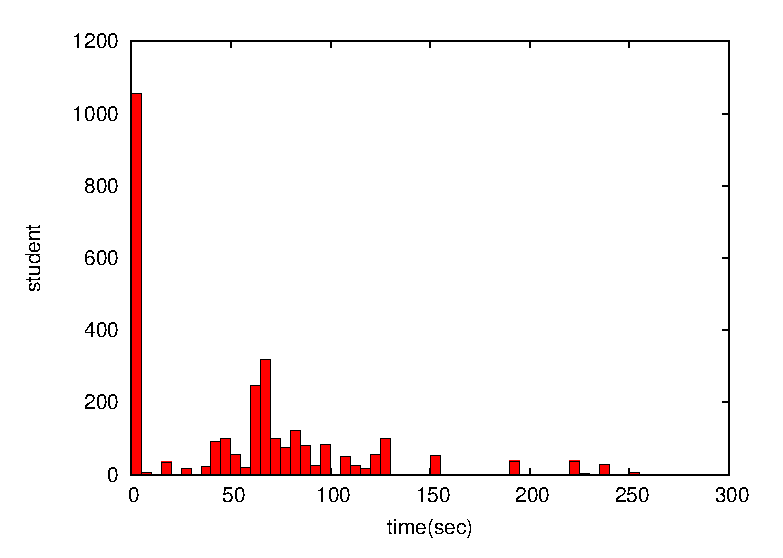
\includegraphics[bb=0 0 390 248,clip,width=\hsize]{oMo345_hist.eps}   
本実験1:春学期月曜午後
\end{center}                                    
\end{minipage}                                 
\begin{minipage}{0.5\hsize}                                            
\begin{center}                              
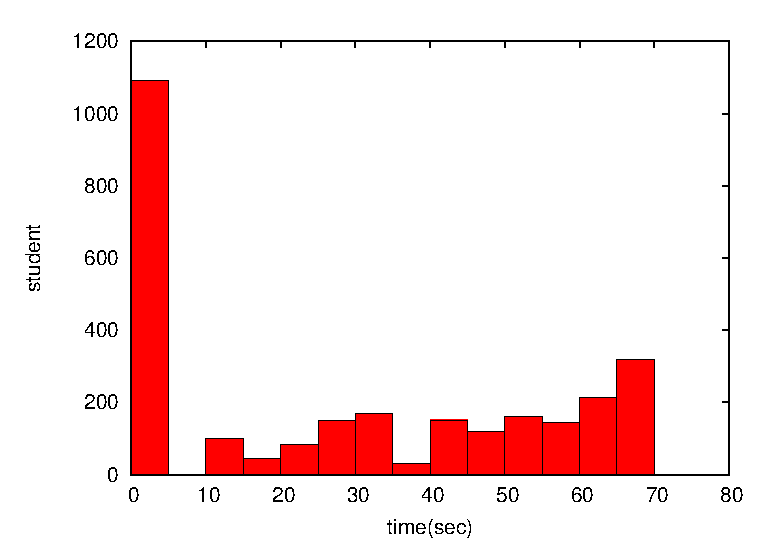
\includegraphics[bb=0 0 390 248,clip,width=\hsize]{oMo345_2_hist.eps}   
本実験2:春学期月曜午後
\end{center}                                    
\end{minipage}                                 
\caption{春学期月曜午後における本実験1と本実験2の移動時間ごとの学生数の比較}                              
\label{hikaku1-2}                                
\end{figure}                                 
\fi

\begin{figure}[thpb]
 \begin{center}
 \hspace{5mm} 
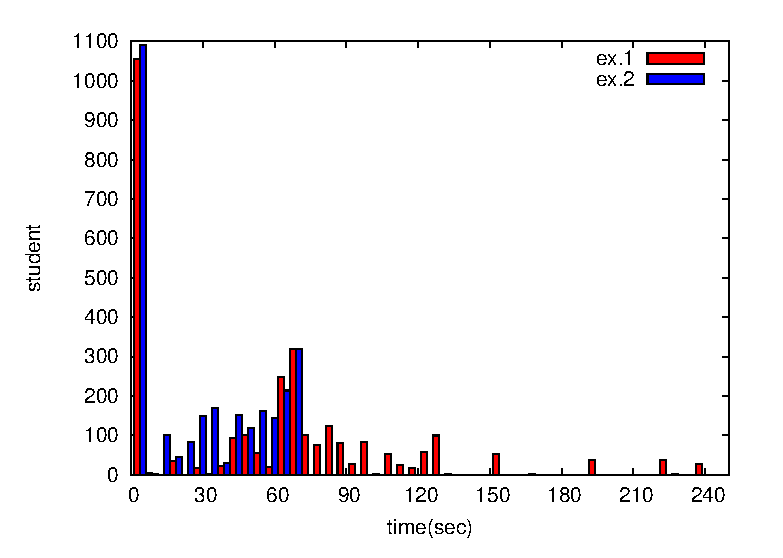
\includegraphics[bb=0 0 390 248,clip,scale=1.0]{omonagahist.eps}
 \hspace{-10mm} 
\vspace{-5mm}
\caption{春学期月曜午後における本実験1と本実験2の移動時間ごとの学生数の比較}                              
  \label{hikaku1-2}
 \end{center}
\end{figure}

表\ref{jikken2_kekka}は,本実験2の実験結果である.
表\ref{jikken2_kekka}より,いずれの曜限における移動時間の最大値とも,本実験1におけるその他の曜限の結果に近い値になっており,特定の授業だけが移動に時間を要していたということが確認できた.
また,図\ref{hikaku1-2}は,春学期月曜午後における本実験1と本実験2の,移動時間(5秒ごと)制の学生数のを比較した図である.
図\ref{hikaku1-2}より,特定の授業を除外することで,その他の授業間の移動時間を大幅に短くできていることがわかる.
この結果より,移動時間が大きくなりそうな授業の教室割当をあらかじめ決めておき,その後に提案手法により残りの授業の教室割当を決めれば,よい割当が求められることがわかる.

\subsection{本実験3:希望教室を設定した実験}
本実験3は,春学期火曜午前のデータに考慮制約2の希望教室を設定して行った実験である.
3つの授業 60190\_oTu1\_1, 60272\_oTu1\_1, 60273\_oTu1\_1にそれぞれ2つの教室4-101,4-102を希望教室として設定している.
すなわち,3つ全ての授業の希望が叶うことはない状況を設定している.

\begin{table}[H]
\caption{春学期火曜午前における本実験1と本実験3の結果の比較}
\label{l:normal_information}
\begin{center}
\begin{tabular}{|r|cccccc|}
\hline
\multicolumn{1}{|c|}{実験} & 最大(秒) & 平均(秒) & 制約数 & 変数の数 & nonzeros & 計算時間(秒)\\
\hline
本実験1       & 76  & 39.4 & 1753 & 2150 & 28679 &  1.04\\
本実験3       & 76  & 47.9 & 1753 & 2150 & 28679 &  1.73\\
\hline
\end{tabular}
\end{center}
\end{table}

\if0
\begin{figure}[htpb]                        
\begin{minipage} {0.5\hsize}                             
\begin{center}                              
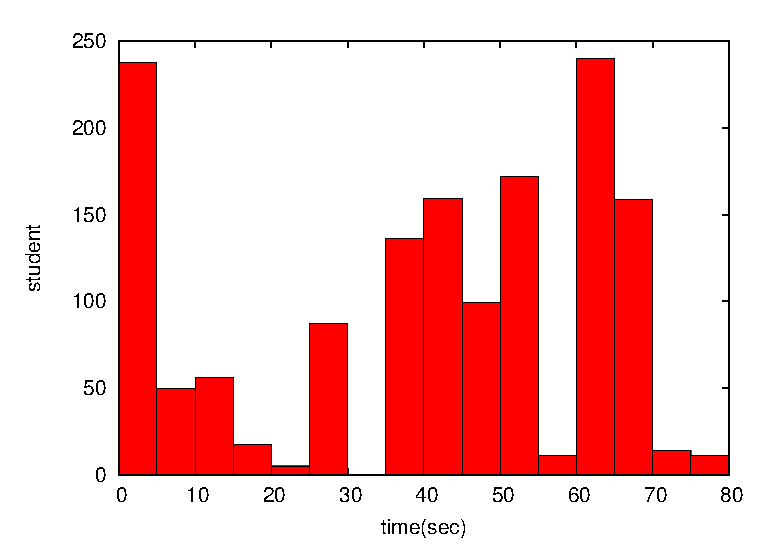
\includegraphics[bb=0 0 390 248,clip,width=\hsize]{oTu12_hist.eps}   
本実験1:春学期火曜午前
\end{center}                                    
\end{minipage}                                 
\begin{minipage}{0.5\hsize}                                            
\begin{center}                              
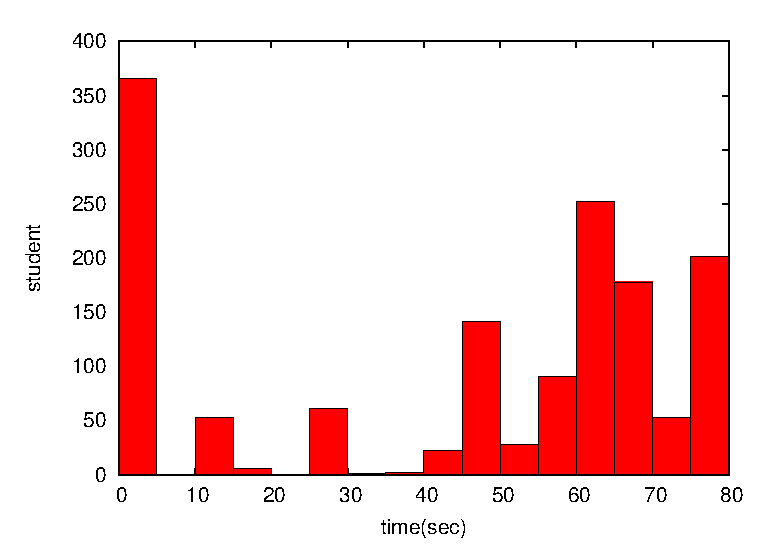
\includegraphics[bb=0 0 390 248,clip,width=\hsize]{oTu12_2_hist.eps}   
本実験3:春学期火曜午前
\end{center}                                    
\end{minipage}                                 
\caption{春学期火曜午前における本実験1と本実験3の移動時間ごとの学生数の比較}                              
\label{hikaku1-3}                                
\end{figure}                                 
\fi

\begin{figure}[thpb]
 \begin{center}
 \hspace{5mm} 
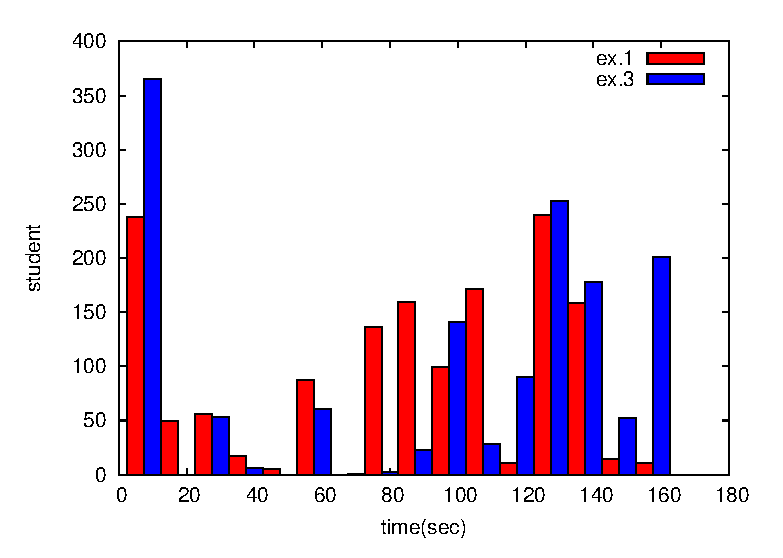
\includegraphics[bb=0 0 390 248,clip,scale=1.0]{otukarehist.eps}
 \hspace{-10mm} 
\vspace{-5mm}
\caption{春学期火曜午前における本実験1と本実験3の移動時間ごとの学生数の比較}                              
  \label{hikaku1-3}
 \end{center}
\end{figure}

表\ref{l:normal_information}は,本実験3の実験結果である.
表\ref{l:normal_information}より,最大の移動時間の最小値は本実験1と同じ値であるが,平均移動時間については本実験1の結果より8.5秒大きくなっていることがわかる.
これは,希望教室を叶えることで,最大の移動時間の最小値には影響しないが,移動が発生してしまったと考えられる.
図\ref{hikaku1-3}は,春学期火曜午前における本実験1と本実験3の,移動時間(5秒ごと)制の学生数のを比較した図である.
図\ref{hikaku1-3}より,移動時間が0秒の学生数も増加しているが,同時に移動時間が大きくなってしまう学生数も増加していることがわかる.
また,目的関数の値を確認すると,希望教室を最大限叶えることができていることがわかった.
この結果より,事前に希望を調べておき,それをできるだけ叶えるような教室割当が求められることがわかった.



\if0
\section{考察}
最大の移動時間を最小化するという方法によって,最大の移動時間を小さくすることができた.
これは,移動時間の最小化をすることができたといえるだろう.
3つの実験によって,本研究のモデルを用いることにより,様々な状況に対応することができるだろう,ということがわかる.
\fi
%\end{document}



\chapter{おわりに}
本研究では,先行研究\cite{先行研究}の定式化の誤りを正し,また異なる視点から教室割当問題を定式化しそれを最適化ソルバーで解くことで,関西大学の理工系学部で開講されている授業に対する,最大の移動時間を最小化するような教室割当を求めることができた.
また,希望教室を設定することで,学生や教員にとって都合のよい教室割当を実現することができることを確認した.
さらに,本研究での教室割当問題の定式化は,関西大学理工系に限らず,様々な大学,学部で使用することができるように作成されている.

付録\ref{huroku}の図\ref{oMo12}~図\ref{oTu12_2}に,全実験における移動時間ごとの学生数を示している.
これらを見ると,最大の移動時間を最小化することで全体の移動時間もある程度小さくなっているものの,移動時間ごとの学生数はまばらになっていることがわかる.
従って,今後の課題として,最大の移動時間を最小化した上で,移動時間の総和の最小化をすることができるのではないかと考えられる.
また,本研究における教室割当においては,本研究で提案した定式化に沿ったデータファイルを作成しなければならない.
従って,本研究における教室割当を求める際に用いることのできるインターフェイスを開発することも必要となるだろう.

\newpage
\chapter*{謝辞}

本研究を進めるに当たり,ご指導頂いた檀寛成助教に深く感謝致します.

また,日常の議論を通じて多くの知識や示唆を頂いたシステムモデリング研究室の皆様へ心から感謝の気持ちと御礼を申し上げて,謝辞にかえさせていただきます.

\begin{flushright} 
平成27年2月13日
\end{flushright} 


\newpage
\begin{thebibliography}{9}

\bibitem{AMPL}
R. Fourer, D. M. Gay,B. W. Kernighan, AMPL A Modeling Language for Mathmatical Programming Second Edition, Thomson Learning (2003).

\bibitem{数理計画入門}
福島雅夫,数理計画入門,朝倉書店 (1996).

\bibitem{CSP}
茨木俊秀,メタヒューリスティクスによる汎用問題解決システムの構築,\\
平成13年度~平成15年度 科学研究費補助金 基盤研究(B)(2)・研究成果報告書 (2004).

\bibitem{CPLEX}
IBM ILOG CPLEX Optimizer,\\
 http://www-01.ibm.com/software/integration/optimization/cplex-optimizer/\\
 (2015年2月9日確認).

\bibitem{dadasenko}
井筒朗,大学における時間割作成問題の汎用ソルバーを用いた求解可能性,関西大学工学部平成19年度卒業論文 (2008).

\bibitem{GLPK}
GLPK -GNU Project- Free Software Foundation (FSF),            
 http://www.gnu.org/software/glpk/ (2015年2月4日確認).

\bibitem{dadasan}
濱田佑,授業再編を考慮した時間割作成ソフトウェアの開発,関西大学環境都市工学部平成25年度卒業論文 (2013).

\bibitem{ハンドブック}
久保幹雄,田村明久,松井知己 編集,応用数理計画ハンドブック,朝倉書店 (2002).

\bibitem{kurousitemituketa}
前川廣太郎,澤勢一史,延原肇,教室移動時間最適化のための群集団移動と多重解像ダイクストラ法を取り入れたマルチエージェントシステムと遺伝的アルゴリズムの開発,筑波大学大学院システム情報工学研究科知能機能システム専攻 (2012).

\bibitem{先行研究}
鈴木健太,移動時間を最小化する教室割当問題の定式化と求解,関西大学環境都市工学部平成26年度卒業論文 (2014).


\end{thebibliography}









\appendix
\def\thechapter{\Alph{chapter}}

\chapter{付録}
\label{huroku}

\section{実験に使用したモデルファイル}
このモデルファイルは本研究で作成したモデルファイルであり,GLPKを用いてLP形式に変換するため,GMPL形式で書いている.そのソースコードを以下に記述する.  

\begin{lstlisting}[label=src1]
##############################
#以下,パラメータ・変数の定義#
##############################

set P;                   #曜限pの集合Pを定義
set P_;                  #曜限pの集合Pを定義
set J;                   #授業jの集合Jを定義
set JN{P};               #P限目の授業
set SJ;                 
set NJ;                 
set I;                   #教室iの集合Iを定義
set SI;                 
set D dimen 2;           #特定の教室を指定する特定の授業の集合Dを定義
set L dimen 2;           #特別連続授業の集合Lを定義
set J_ ;                 #教室希望を出している授業の集合
set I_{J_};              #授業j_の希望教室の集合
                        
param m {I};             #教室iの定員
param n {J};             #講義jの受講者数
param t {I,I};           #教室i1から教室i2の所要移動時間
param r;                 #移動時間の限界値
param d {J,J} binary;    #p限目に授業j1を,(p+1)限目に授業j2を受講する学生の存在を示すパラメータd_j1,j2の定義
param q {J,J};           #p限目に授業j1を,(p+1)限目に授業j2を受講する学生数
param z;                 #混雑が起きると予想される人数

var u {I,J} binary;      #授業jに教室iを割り当てる
var alpha {J,J} binary;  #考慮制約1の違反の指標


set PC;                  #考慮制約の番号  
var K {PC};              #各考慮制約の違反指標の合計 

#各考慮制約の重みを示すパラメータpa_pcを定義
param pa {PC};


##########################
## 以下,制約条件の定義 ##
##########################

#絶対制約1(各曜限の各教室に授業はひとつ)

subject to C1{p in P, i in I}:

	sum{j in JN[p]} u[i,j] <= 1;

#絶対制約2(各授業には教室をひとつ)

 subject to C2{p in P, j in JN[p]}:

	sum{i in I} u[i,j] == 1;

#絶対制約3(教室の定員を守る)

subject to C3{p in P, j in JN[p]}:

	sum{i in I} u[i,j] * m[i] >= n[j];

#絶対制約4(特定の授業は指定した教室で行う)

subject to C4{(i, j) in D}:

	u[i,j] == 1;

#絶対制約4_2(特殊教室で一般授業を行わない)

subject to C4_2{p in P, j in JN[p], i in SI:  j not in SJ }:

	u[i,j] == 0;

#絶対制約5(移動時間は指定した時間以内)

subject to C5{p_ in P_, i1 in I,i2 in I,j1 in JN[p_],j2 in JN[p_+1]:t[i1, i2] >= r && d[j1,j2] == 1}:

	u[i1,j1] + u[i2,j2] <= 1;

#絶対制約6(特別連続授業は同じ教室で受講)

subject to C6{i in I,(j1,j2) in L}:

	u[i,j1] == u[i,j2];

#考慮制約1(教室内の人が入れ替わる際の混雑)

subject to C7{p_ in P_,i in I,j1 in JN[p_],j2 in JN[p_+1]: ((n[j1]-q[j1,j2]) + (n[j2]-q[j1,j2])) - z > 0 && d[j1,j2]==1}:

	(u[i,j1] + u[i,j2]-1) <= alpha[j1,j2];

subject to S1 : 
       K[1] = sum{p_ in P_,j1 in JN[p_],j2 in JN[p_+1]} alpha[j1,j2];

#考慮制約2(希望教室)

subject to S2 :
	K[2] =  sum{j_ in J_,i_ in I_[j_]}  u[i_,j_];

#目的関数の定義

minimize func :  sum{pc in PC} (pa[pc] * K[pc]);
\end{lstlisting}

\newpage
\section{実験に使用したパラメータ}
\label{hurokupara}
表\ref{tokushu},表\ref{paramt}は,本研究で用いているパラメータである.
\begin{table}[!h]
\begin{center}
\caption{本研究で扱っている特殊教室}
\label{tokushu}
\begin{tabular}{|c|c|}
\hline
特殊教室名 & モデル変換名\\
\hline\hline
4-オープンデザイン1教室          &   4-od1 \\
4-オープンデザイン2教室          &   4-od2 \\
4-第4学舎情報処理室              &   4-0001\\
4-デザインルーム1                &   4-0002\\
4-デザインルーム2                &   4-0003\\
4-第二製図室                      &   4-0004\\
4-シスマネ実験室3(1号教1F)       &   4-0005\\
4-化学物質実験場(第4実1F)    &   4-0006\\
4-先端マテリアル実験場(第4実1F)   &   4-0007\\
4-生物工学実験室2(第4実BF)  &   4-0008\\
4-生物工学実験室1(第4実3F)  &   4-0009\\
4-電気工学実験場(第1実3F)    &   4-0010\\
4-物理学実験場(2号実2F)      &   4-0011\\
4-物理共同演習室(2号実BF)    &   4-0012\\
4-共同化学実験場Ⅰ(第2実2F)  &   4-0013\\
4-共同化学実験場Ⅱ(第2実3F)  &   4-0014\\
4-化学工学科実験場(第4実BF)  &   4-0015\\
4-機械共同実験室(第5実1F)    &   4-0016\\
4-電子工学実験室(第5実3F)    &   4-0017\\
4-物理学生実験場(第5実BF)    &   4-0018\\
4-建築実験室(コ・土第6実1F)  &   4-0019\\
4-都市実験実習場(第6実3F)    &   4-0020\\
4-機械実習工場(第6実3F)      &   4-0021\\
\hline
\end{tabular}
\end{center}
\end{table}


\begin{table}[htbp]
 \begin{center}
\caption{教室間の移動時間($t_{i_1,i_2}$)}
\label{paramt}
  {\tiny
  \begin{tabular}{lccccccccccccccccc}
%
\hline
 & 101 & 102 & 103 & 104 & 105 & 106 & 107 & 201A
   & 202 & 203 & 204 & 205 & 206 & 207 & 208 &
   209 & 210 \\
\hline
102 & 16 &  &  &  &  &  &  &  &  &  &  &  &  &  &  &  &  \\
103 & 18 & 2 &  &  &  &  &  &  &  &  &  &  &  &  &  &  &  \\
104 & 51 & 35 & 33 &  &  &  &  &  &  &  &  &  &  &  &  &  &  \\
105 & 66 & 50 & 48 & 15 &  &  &  &  &  &  &  &  &  &  &  &  &  \\
106 & 78 & 62 & 60 & 27 & 11 &  &  &  &  &  &  &  &  &  &  &  &  \\
107 & 81 & 65 & 63 & 30 & 14 & 3 &  &  &  &  &  &  &  &  &  &  &  \\
201A & 46 & 62 & 64 & 97 & 112 & 123 & 126 &  &  &  &  &  &  &  &  &
								   &  \\
202 & 48 & 64 & 66 & 83 & 73 & 84 & 87 & 39 &  &  &  &  &  &  &  &  &  \\
203 & 57 & 73 & 68 & 74 & 64 & 75 & 78 & 48 & 9 &  &  &  &  &  &  &
								   &  \\
204 & 66 & 61 & 59 & 65 & 55 & 66 & 69 & 57 & 18 & 9 &  &  &  &  &  &
								   &  \\
205 & 74 & 53 & 51 & 57 & 47 & 58 & 61 & 65 & 26 & 17 & 8 &  &  &  &
							       &  &  \\
206 & 83 & 44 & 42 & 48 & 38 & 49 & 52 & 74 & 35 & 26 & 17 & 9 &  &
							   &  &  &  \\
207 & 100 & 55 & 53 & 59 & 49 & 60 & 63 & 91 & 52 & 43 & 34 & 25 & 16
						       &  &  &  &  \\
208 & 116 & 71 & 69 & 75 & 65 & 67 & 64 & 107 & 68 & 59 & 50 & 41 &
						       32 & 16 &  &  &  \\
209 & 127 & 82 & 80 & 86 & 76 & 56 & 53 & 118 & 79 & 70 & 61 & 52 &
						       43 & 27 & 11 &  &  \\
210 & 130 & 85 & 83 & 89 & 79 & 53 & 50 & 121 & 82 & 73 & 64 & 55 &
						       46 & 30 & 14 & 3
								   &  \\
301 & 62 & 78 & 80 & 108 & 98 & 109 & 112 & 52 & 44 & 53 & 62 & 77 &
						       68 & 84 & 101 &
								   112 &
								       115 \\
302 & 74 & 90 & 90 & 96 & 86 & 97 & 100 & 64 & 56 & 65 & 74 & 65 & 56
						       & 72 & 89 & 100 &
								       103 \\
303 & 87 & 79 & 77 & 83 & 73 & 84 & 87 & 77 & 69 & 69 & 60 & 52 & 43
						       & 59 & 76 & 87 &
								       90 \\
304 & 99 & 67 & 65 & 71 & 61 & 72 & 75 & 89 & 81 & 57 & 48 & 40 & 31
						       & 47 & 64 & 75 &
								       78 \\
305 & 120 & 76 & 74 & 80 & 70 & 81 & 84 & 110 & 102 & 66 & 57 & 49 &
						       40 & 56 & 73 & 84
								   & 87 \\
306 & 136 & 92 & 90 & 96 & 86 & 96 & 93 & 126 & 118 & 82 & 73 & 65 &
						       56 & 72 & 89 & 78
								   & 75 \\
307 & 161 & 117 & 115 & 121 & 111 & 71 & 68 & 151 & 143 & 107 & 98 &
						   90 & 81 & 97 & 64 &
								   53 &
								       50 \\
308 & 165 & 121 & 119 & 125 & 115 & 67 & 64 & 155 & 147 & 111 & 102 &
						   94 & 85 & 101 & 60 &
								   49 &
								       46 \\
401 & 85 & 101 & 103 & 125 & 115 & 126 & 129 & 75 & 67 & 76 & 102 &
						   94 & 84 & 101 & 118 &
								   129 &
								       132 \\
402 & 97 & 109 & 107 & 113 & 103 & 114 & 117 & 87 & 79 & 88 & 90 & 82
						   & 72 & 89 & 106 & 117
								   & 120 \\
403 & 109 & 97 & 95 & 101 & 91 & 102 & 105 & 99 & 91 & 87 & 78 & 70 &
						       60 & 77 & 94 &
								   105 &
								       108 \\
404 & 120 & 86 & 84 & 90 & 80 & 91 & 94 & 110 & 102 & 76 & 67 & 59 &
						       49 & 66 & 83 & 94
								   & 97 \\
405 & 141 & 94 & 92 & 98 & 88 & 99 & 102 & 131 & 123 & 84 & 75 & 67 &
						       57 & 74 & 91 & 97
								   & 95 \\
406 & 156 & 109 & 107 & 113 & 103 & 100 & 97 & 146 & 138 & 99 & 90 &
						   82 & 72 & 89 & 93 &
								   82 &
								       79 \\
407 & 168 & 121 & 119 & 125 & 115 & 88 & 85 & 158 & 150 & 111 & 102 &
						   94 & 84 & 101 & 81 &
								   70 &
								       67 \\
408 & 171 & 124 & 122 & 128 & 118 & 85 & 82 & 161 & 153 & 114 & 105 &
						   97 & 87 & 104 & 78 &
								   67 &
								       64 \\
501 & 95 & 111 & 113 & 146 & 161 & 172 & 175 & 93 & 85 & 94 & 103 &
						   111 & 120 & 136 & 152
							       & 163 &
								       166 \\
3101 & 111 & 95 & 93 & 60 & 45 & 34 & 30 & 157 & 118 & 109 & 100 & 91
						   & 82 & 93 & 141 & 83
								   & 80 \\
3201 & 140 & 124 & 122 & 89 & 74 & 63 & 59 & 186 & 147 & 138 & 129 &
						   120 & 111 & 122 & 170
							       & 112 &
								       109 \\
3202 & 144 & 128 & 126 & 93 & 78 & 67 & 63 & 190 & 151 & 142 & 133 &
						   124 & 115 & 126 & 174
							       & 116 &
								       113 \\
4A & 229 & 245 & 247 & 280 & 295 & 306 & 309 & 275 & 277 & 286 & 295
					       & 303 & 312 & 329 & 345 &
								   356 &
								       336 \\
4B & 215 & 231 & 233 & 266 & 281 & 292 & 295 & 261 & 263 & 272 & 281
					       & 289 & 298 & 315 & 331 &
								   342 &
								       322 \\
502 & 130 & 114 & 122 & 128 & 143 & 155 & 158 & 162 & 123 & 114 & 105
					       & 97 & 88 & 99 & 115 &
								   126 &
								       129 \\
201B & 46 & 62 & 64 & 97 & 112 & 123 & 126 & 2 & 39 & 48 & 57 & 65 &
						       74 & 91 & 107 &
								   118 &
								       121 \\
3401 & 174 & 158 & 166 & 123 & 108 & 97 & 93 & 210 & 181 & 172 & 163 &
						   154 & 145 & 156 & 204
							       & 146 &
								       143 \\
3402 & 179 & 163 & 171 & 128 & 113 & 102 & 98 & 215 & 186 & 177 & 169
					       & 159 & 150 & 161 & 209 &
								   151 &
								       148 \\
3403 & 184 & 188 & 176 & 133 & 118 & 117 & 113 & 220 & 191 & 182 & 173
					       & 164 & 155 & 166 & 214 &
								   156 &
								       153 \\
od1 & 212 & 196 & 194 & 161 & 145 & 134 & 124 & 184 & 145 & 136 & 127
					       & 119 & 110 & 93 & 76 &
								   65 &
								       60 \\
od2 & 130 & 114 & 122 & 128 & 143 & 155 & 158 & 162 & 123 & 114 & 105
					       & 97 & 88 & 99 & 115 &
								   126 &
								       129 \\
0001 & 56 & 72 & 74 & 107 & 122 & 133 & 136 & 15 & 49 & 58 & 67 & 75 &
						       84 & 101 & 117 &
								   128 &
								       131 \\
0002 & 154 & 158 & 146 & 103 & 88 & 87 & 83 & 190 & 161 & 152 & 143 &
						   134 & 125 & 136 & 184
							       & 126 &
								       123 \\
0003 & 152 & 156 & 144 & 101 & 86 & 85 & 81 & 188 & 159 & 150 & 141 &
						   132 & 123 & 134 & 182
							       & 124 &
								       121 \\
0004 & 125 & 109 & 117 & 123 & 138 & 150 & 153 & 157 & 118 & 109 & 100
					       & 92 & 83 & 94 & 110 &
								   121 &
								       124 \\
0005 & 126 & 142 & 144 & 177 & 192 & 203 & 206 & 82 & 119 & 128 & 137
					       & 145 & 154 & 171 & 187 &
								   198 &
								       201 \\
0006 & 185 & 201 & 203 & 236 & 251 & 262 & 265 & 231 & 233 & 242 & 251
					       & 259 & 298 & 185 & 301 &
								   312 &
								       192 \\
0007 & 195 & 211 & 213 & 246 & 261 & 272 & 275 & 241 & 243 & 252 & 261
					       & 269 & 308 & 195 & 311 &
								   322 &
								       202 \\
0008 & 190 & 206 & 208 & 241 & 255 & 267 & 270 & 236 & 238 & 247 & 256
					       & 264 & 303 & 190 & 306 &
								   317 &
								       197 \\
0009 & 195 & 211 & 213 & 246 & 261 & 272 & 275 & 241 & 243 & 252 & 261
					       & 269 & 308 & 195 & 311 &
								   322 &
								       202 \\
0010 & 200 & 216 & 218 & 251 & 266 & 278 & 281 & 246 & 248 & 257 & 266
					       & 274 & 283 & 300 & 316 &
								   327 &
								       330 \\
0011 & 141 & 157 & 159 & 192 & 207 & 219 & 222 & 227 & 189 & 198 & 207
					       & 215 & 224 & 241 & 257 &
								   268 &
								       271 \\
0012 & 100 & 106 & 108 & 151 & 166 & 178 & 181 & 146 & 148 & 157 & 166
					       & 174 & 183 & 200 & 216 &
								   227 &
								       230 \\
0013 & 212 & 228 & 240 & 263 & 278 & 280 & 293 & 258 & 260 & 269 & 278
					       & 286 & 295 & 312 & 328 &
								   339 &
								       342 \\
0014 & 233 & 249 & 261 & 284 & 299 & 301 & 314 & 279 & 281 & 290 & 299
					       & 307 & 316 & 333 & 349 &
								   360 &
								       363 \\
0015 & 205 & 221 & 223 & 256 & 270 & 292 & 285 & 251 & 253 & 262 & 271
					       & 279 & 318 & 205 & 321 &
								   332 &
								       212 \\
0016 & 245 & 261 & 253 & 296 & 311 & 322 & 325 & 291 & 293 & 302 & 311
					       & 319 & 358 & 245 & 361 &
								   372 &
								       252 \\
0017 & 277 & 293 & 285 & 228 & 343 & 354 & 357 & 343 & 345 & 334 & 343
					       & 352 & 390 & 277 & 393 &
								   405 &
								       284 \\
0018 & 265 & 278 & 270 & 213 & 328 & 349 & 342 & 328 & 330 & 329 & 328
					       & 337 & 375 & 262 & 378 &
								   390 &
								       269 \\
0019 & 321 & 337 & 339 & 372 & 387 & 399 & 402 & 367 & 369 & 378 & 387
					       & 395 & 404 & 421 & 437 &
								   448 &
								       451 \\
0020 & 336 & 352 & 354 & 387 & 402 & 414 & 417 & 382 & 384 & 393 & 402
					       & 410 & 419 & 436 & 452 &
								   463 &
								       466 \\
0021 & 326 & 342 & 344 & 377 & 392 & 404 & 407 & 372 & 374 & 383 & 392
					       & 400 & 409 & 426 & 442 &
								   453 &
								       456 \\
\hline
%
  \end{tabular}
  }
 \end{center}
\end{table}

\newpage

\begin{table}[htbp]
 \begin{center}
  {\tiny
  \begin{tabular}{lccccccccccccccccc}
%
\hline
 & 301 & 302 & 303 & 304 & 305 & 306 & 307 & 308 & 401 & 402 & 403 & 404
   & 405 & 406 & 407 & 408 & 501 \\
\hline
302 & 12 &  &  &  &  &  &  &  &  &  &  &  &  &  &  &  &  \\
303 & 25 & 13 &  &  &  &  &  &  &  &  &  &  &  &  &  &  &  \\
304 & 37 & 25 & 12 &  &  &  &  &  &  &  &  &  &  &  &  &  &  \\
305 & 58 & 46 & 33 & 21 &  &  &  &  &  &  &  &  &  &  &  &  &  \\
306 & 74 & 62 & 49 & 37 & 16 &  &  &  &  &  &  &  &  &  &  &  &  \\
307 & 99 & 87 & 74 & 62 & 41 & 25 &  &  &  &  &  &  &  &  &  &  &  \\
308 & 103 & 91 & 78 & 66 & 45 & 29 & 4 &  &  &  &  &  &  &  &  &  &  \\
401 & 37 & 49 & 78 & 66 & 75 & 91 & 116 & 120 &  &  &  &  &  &  &  &  &  \\
402 & 49 & 61 & 66 & 54 & 63 & 79 & 104 & 108 & 12 &  &  &  &  &  &  &
								   &  \\
403 & 61 & 67 & 54 & 42 & 51 & 67 & 92 & 96 & 24 & 12 &  &  &  &  &  &
								   &  \\
404 & 68 & 56 & 43 & 31 & 40 & 56 & 81 & 85 & 35 & 23 & 11 &  &  &  &  &
								   &  \\
405 & 76 & 64 & 51 & 39 & 48 & 64 & 83 & 79 & 56 & 44 & 32 & 21 &  &  &
							       &  &  \\
406 & 91 & 79 & 66 & 54 & 63 & 79 & 68 & 64 & 71 & 59 & 47 & 36 & 15 &
							   &  &  &  \\
407 & 103 & 91 & 78 & 66 & 75 & 91 & 56 & 52 & 83 & 71 & 59 & 48 & 27 &
							   12 &  &  &  \\
408 & 106 & 94 & 81 & 69 & 78 & 94 & 53 & 49 & 86 & 74 & 62 & 51 & 30 &
							   15 & 3 &  &  \\
501 & 55 & 67 & 80 & 84 & 105 & 121 & 146 & 150 & 32 & 44 & 56 & 67 & 88
						       & 103 & 115 & 118
								   &  \\
3101 & 168 & 156 & 143 & 131 & 140 & 156 & 98 & 94 & 170 & 173 & 161 &
						   150 & 158 & 173 & 115
							       & 108 &
								       205 \\
3201 & 197 & 185 & 172 & 160 & 169 & 185 & 127 & 123 & 199 & 202 & 190 &
						   179 & 187 & 202 & 144
							       & 137 &
								       234 \\
3202 & 201 & 189 & 176 & 164 & 173 & 189 & 131 & 127 & 203 & 206 & 194 &
						   183 & 191 & 206 & 148
							       & 141 &
								       238 \\
4A & 292 & 304 & 324 & 312 & 321 & 337 & 362 & 366 & 299 & 327 & 342 &
						   331 & 339 & 354 & 366
							       & 369 &
								       324 \\
4B & 278 & 290 & 310 & 298 & 307 & 323 & 348 & 352 & 285 & 313 & 328 &
						   317 & 325 & 340 & 352
							       & 355 &
								       310 \\
502 & 106 & 94 & 81 & 69 & 78 & 94 & 119 & 123 & 86 & 74 & 62 & 51 & 30
						       & 48 & 57 & 60 &
								       118 \\
201B & 52 & 64 & 77 & 89 & 110 & 126 & 151 & 155 & 75 & 87 & 99 & 110 &
						       131 & 146 & 158 &
								   161 &
								       93 \\
3401 & 231 & 219 & 206 & 194 & 203 & 219 & 161 & 157 & 233 & 236 & 224 &
						   213 & 221 & 236 & 178
							       & 171 &
								       268 \\
3402 & 236 & 224 & 211 & 199 & 208 & 224 & 166 & 162 & 238 & 241 & 229 &
						   218 & 226 & 241 & 183
							       & 176 &
								       273 \\
3403 & 241 & 229 & 216 & 104 & 213 & 229 & 171 & 167 & 243 & 246 & 234 &
						   223 & 231 & 246 & 188
							       & 181 &
								       278 \\
od1 & 152 & 140 & 127 & 115 & 94 & 77 & 60 & 49 & 112 & 100 & 88 & 76 &
						       56 & 40 & 31 & 20
								   & 144 \\
od2 & 106 & 94 & 81 & 69 & 78 & 94 & 119 & 123 & 86 & 74 & 62 & 51 & 30
						       & 48 & 57 & 60 &
								       118 \\
0001 & 62 & 74 & 87 & 99 & 120 & 136 & 161 & 165 & 85 & 97 & 109 & 120 &
						       141 & 156 & 168 &
								   171 &
								       103 \\
0002 & 211 & 199 & 186 & 64 & 183 & 199 & 141 & 137 & 213 & 216 & 204 &
						   193 & 201 & 216 & 158
							       & 151 &
								       248 \\
0003 & 209 & 197 & 184 & 62 & 181 & 197 & 139 & 135 & 211 & 214 & 202 &
						   191 & 199 & 214 & 156
							       & 149 &
								       246 \\
0004 & 101 & 89 & 76 & 64 & 73 & 89 & 114 & 118 & 81 & 69 & 57 & 46 & 25
						       & 43 & 52 & 55 &
								       113 \\
0005 & 132 & 144 & 157 & 169 & 190 & 806 & 231 & 235 & 255 & 167 & 179 &
						   190 & 211 & 226 & 238
							       & 241 &
								       173 \\
0006 & 248 & 260 & 180 & 268 & 277 & 293 & 318 & 322 & 255 & 283 & 298 &
						   287 & 295 & 310 & 322
							       & 325 &
								       280 \\
0007 & 258 & 250 & 190 & 288 & 287 & 303 & 328 & 332 & 265 & 293 & 308 &
						   297 & 305 & 320 & 332
							       & 335 &
								       290 \\
0008 & 253 & 245 & 185 & 283 & 282 & 298 & 323 & 327 & 260 & 288 & 303 &
						   292 & 300 & 315 & 327
							       & 330 &
								       285 \\
0009 & 258 & 250 & 190 & 288 & 287 & 303 & 328 & 332 & 265 & 293 & 308 &
						   297 & 305 & 320 & 332
							       & 335 &
								       290 \\
0010 & 262 & 274 & 287 & 299 & 320 & 336 & 361 & 365 & 285 & 297 & 309 &
						   320 & 341 & 356 & 368
							       & 371 &
								       295 \\
0011 & 203 & 215 & 228 & 140 & 261 & 277 & 302 & 306 & 226 & 238 & 250 &
						   261 & 282 & 297 & 309
							       & 312 &
								       236 \\
0012 & 162 & 174 & 187 & 199 & 220 & 236 & 261 & 265 & 185 & 197 & 209 &
						   220 & 241 & 256 & 268
							       & 271 &
								       195 \\
0013 & 272 & 286 & 299 & 311 & 332 & 348 & 373 & 377 & 297 & 309 & 321 &
						   332 & 353 & 368 & 380
							       & 383 &
								       307 \\
0014 & 293 & 307 & 320 & 332 & 353 & 369 & 394 & 398 & 318 & 330 & 342 &
						   353 & 374 & 389 & 401
							       & 404 &
								       328 \\
0015 & 268 & 260 & 200 & 298 & 297 & 313 & 338 & 342 & 275 & 303 & 318 &
						   307 & 315 & 330 & 342
							       & 345 &
								       300 \\
0016 & 308 & 320 & 240 & 328 & 337 & 353 & 378 & 382 & 375 & 343 & 358 &
						   357 & 355 & 370 & 382
							       & 385 &
								       340 \\
0017 & 340 & 352 & 262 & 360 & 369 & 384 & 410 & 414 & 407 & 375 & 390 &
						   389 & 387 & 402 & 414
							       & 417 &
								       372 \\
0018 & 315 & 337 & 247 & 345 & 354 & 369 & 395 & 399 & 392 & 360 & 375 &
						   374 & 372 & 397 & 399

							       & 402 &
								       357 \\
0019 & 383 & 395 & 408 & 420 & 441 & 457 & 482 & 486 & 406 & 418 & 430 &
						   441 & 462 & 477 & 489
							       & 492 &
								       416 \\
0020 & 398 & 410 & 423 & 435 & 456 & 472 & 497 & 501 & 421 & 423 & 445 &
						   456 & 477 & 492 & 504
							       & 507 &
								       431 \\
0021 & 388 & 400 & 413 & 425 & 446 & 462 & 487 & 491 & 411 & 413 & 435 &
						   446 & 467 & 482 & 494
							       & 497 &
								       421 \\
\hline
%
  \end{tabular}
  }
 \end{center}
\end{table}


\begin{table}[htbp]
 \begin{center}
  {\tiny
  \begin{tabular}{lccccccccccccccccc}
%
\hline
 & 3101 & 3201 & 3202 & 4A & 4B & 502 & 201B & 3401 & 3402 & 3403 & od1
   & od2 & 0001 & 0002 & 0003 & 0004 & 0005 \\
\hline
3201 & 29 &  &  &  &  &  &  &  &  &  &  &  &  &  &  &  &  \\
3202 & 33 & 4 &  &  &  &  &  &  &  &  &  &  &  &  &  &  &  \\
4A & 340 & 369 & 373 &  &  &  &  &  &  &  &  &  &  &  &  &  &  \\
4B & 326 & 355 & 359 & 14 &  &  &  &  &  &  &  &  &  &  &  &  &  \\
502 & 188 & 217 & 221 & 369 & 355 &  &  &  &  &  &  &  &  &  &  &  &  \\
201B & 157 & 186 & 190 & 275 & 261 & 123 &  &  &  &  &  &  &  &  &  &  &  \\
3401 & 63 & 34 & 30 & 403 & 389 & 247 & 220 &  &  &  &  &  &  &  &  &  &  \\
3402 & 68 & 39 & 35 & 408 & 394 & 252 & 225 & 5 &  &  &  &  &  &  &  &
								   &  \\
3403 & 73 & 44 & 40 & 413 & 399 & 257 & 230 & 10 & 5 &  &  &  &  &  &  &
								   &  \\
od1 & 214 & 215 & 250 & 395 & 381 & 17 & 145 & 245 & 250 & 255 &  &  &
						       &  &  &  &  \\
od2 & 188 & 217 & 221 & 369 & 355 & 3 & 123 & 247 & 252 & 257 & 7 &  &
						       &  &  &  &  \\
0001 & 167 & 196 & 200 & 285 & 271 & 133 & 10 & 230 & 235 & 240 & 155 &
						   133 &  &  &  &  &  \\
0002 & 43 & 24 & 20 & 383 & 369 & 227 & 210 & 20 & 25 & 15 & 225 & 227 &
						       200 &  &  &  &  \\
0003 & 41 & 22 & 18 & 381 & 367 & 225 & 208 & 18 & 23 & 13 & 223 & 225 &
						       198 & 2 &  &  &  \\
0004 & 183 & 212 & 216 & 364 & 350 & 6 & 118 & 242 & 247 & 252 & 12 & 8
						   & 128 & 222 & 220 &
								   &  \\
0005 & 237 & 266 & 270 & 149 & 133 & 203 & 80 & 300 & 305 & 310 & 225 &
						   203 & 90 & 290 & 288
							       & 195 &  \\
0006 & 296 & 325 & 329 & 44 & 30 & 325 & 231 & 359 & 364 & 369 & 351 &
						   325 & 241 & 339 & 337
							       & 320 &
								       103 \\
0007 & 306 & 335 & 339 & 54 & 40 & 335 & 241 & 369 & 374 & 379 & 361 &
						   335 & 251 & 349 & 347
							       & 330 &
								       113 \\
0008 & 301 & 330 & 334 & 49 & 35 & 330 & 236 & 364 & 369 & 374 & 356 &
						   330 & 246 & 344 & 342
							       & 325 &
								       108 \\
0009 & 306 & 335 & 339 & 24 & 20 & 335 & 241 & 369 & 374 & 379 & 361 &
						   335 & 251 & 349 & 347
							       & 330 &
								       113 \\
0010 & 311 & 340 & 344 & 129 & 115 & 33 & 246 & 374 & 379 & 384 & 412 &
						   330 & 256 & 354 & 352
							       & 325 &
								       326 \\
0011 & 252 & 261 & 285 & 190 & 176 & 271 & 187 & 315 & 320 & 315 & 353 &
						   271 & 197 & 295 & 293
							       & 266 &
								       187 \\
0012 & 211 & 240 & 244 & 29 & 215 & 230 & 146 & 274 & 279 & 284 & 212 &
						   230 & 156 & 254 & 252
							       & 225 &
								       226 \\
0013 & 323 & 352 & 356 & 141 & 127 & 342 & 258 & 386 & 391 & 396 & 424 &
						   342 & 268 & 366 & 364
							       & 337 &
								       338 \\
0014 & 344 & 373 & 377 & 162 & 148 & 363 & 279 & 407 & 412 & 417 & 445 &
						   363 & 289 & 387 & 385
							       & 358 &
								       359 \\
0015 & 316 & 345 & 349 & 64 & 50 & 345 & 251 & 379 & 384 & 389 & 371 &
						   345 & 261 & 369 & 357
							       & 340 &
								       123 \\
0016 & 356 & 385 & 389 & 104 & 90 & 385 & 291 & 419 & 424 & 429 & 411 &
						   385 & 301 & 399 & 397
							       & 380 &
								       163 \\
0017 & 388 & 417 & 421 & 136 & 122 & 417 & 323 & 452 & 456 & 461 & 443 &
						   417 & 333 & 431 & 439
							       & 412 &
								       195 \\
0018 & 373 & 402 & 406 & 121 & 107 & 402 & 308 & 437 & 441 & 446 & 428 &
						   402 & 318 & 416 & 424
							       & 397 &
								       180 \\
0019 & 432 & 461 & 465 & 250 & 236 & 451 & 367 & 495 & 500 & 505 & 533 &
						   451 & 477 & 475 & 473
							       & 446 &
								       447 \\
0020 & 447 & 476 & 480 & 265 & 251 & 466 & 382 & 510 & 515 & 520 & 548 &
						   466 & 492 & 490 & 488
							       & 461 &
								       462 \\
0021 & 437 & 466 & 470 & 255 & 241 & 456 & 372 & 500 & 505 & 510 & 538 &
						   456 & 482 & 480 & 478
							       & 451 &
								       452 \\
\hline
%
  \end{tabular}
  }
 \end{center}
\end{table}

\begin{table}[htbp]
 \begin{center}
  {\tiny
  \begin{tabular}{lccccccccccccccc}
%
\hline
 & 0006 & 0007 & 0008 & 0009 & 0010 & 0011 & 0012 & 0013 & 0014 & 0015 &
   0016 & 0017 & 0018 & 0019 & 0020 \\
\hline
0007 & 10 &  &  &  &  &  &  &  &  &  &  &  &  &  &  \\
0008 & 15 & 10 &  &  &  &  &  &  &  &  &  &  &  &  &  \\
0009 & 20 & 24 & 45 &  &  &  &  &  &  &  &  &  &  &  &  \\
0010 & 115 & 125 & 120 & 125 &  &  &  &  &  &  &  &  &  &  &  \\
0011 & 176 & 186 & 181 & 186 & 145 &  &  &  &  &  &  &  &  &  &  \\
0012 & 215 & 225 & 220 & 225 & 165 & 183 &  &  &  &  &  &  &  &  &  \\
0013 & 127 & 137 & 132 & 137 & 77 & 152 & 144 &  &  &  &  &  &  &  &  \\
0014 & 148 & 158 & 153 & 158 & 98 & 183 & 165 & 30 &  &  &  &  &  &  &  \\
0015 & 30 & 25 & 15 & 60 & 135 & 196 & 235 & 147 & 168 &  &  &  &  &  &  \\
0016 & 60 & 70 & 75 & 80 & 175 & 296 & 275 & 187 & 208 & 90 &  &  &  &
							   &  \\
0017 & 92 & 102 & 107 & 112 & 207 & 208 & 302 & 219 & 240 & 122 & 32 &
						   &  &  &  \\
0018 & 77 & 87 & 92 & 97 & 192 & 193 & 287 & 204 & 225 & 107 & 17 & 15 &
						       &  &  \\
0019 & 236 & 246 & 241 & 246 & 185 & 280 & 263 & 132 & 153 & 256 & 296 &
						   328 & 313 &  &  \\
0020 & 251 & 261 & 256 & 261 & 200 & 295 & 278 & 147 & 148 & 271 & 311 &
						   343 & 328 & 60 &  \\
0021 & 241 & 251 & 246 & 251 & 190 & 285 & 268 & 137 & 128 & 261 & 301 &
						   333 & 318 & 50 & 10 \\
\hline
%
  \end{tabular}
  }
 \end{center}
\end{table}

\newpage
\section{移動時間ごとの学生数}
図\ref{oMo12}~図\ref{otukaresan}は,各本実験における最適解での移動時間ごとの学生数の推移を示している.
\if0
\documentclass[a4paper,10pt]{jarticle}
\usepackage[dvips]{graphicx}
\usepackage{amsmath}

\begin{document}
\fi

\begin{figure}[htpb]                        
\begin{minipage} {0.5\hsize}                             
\begin{center}                              
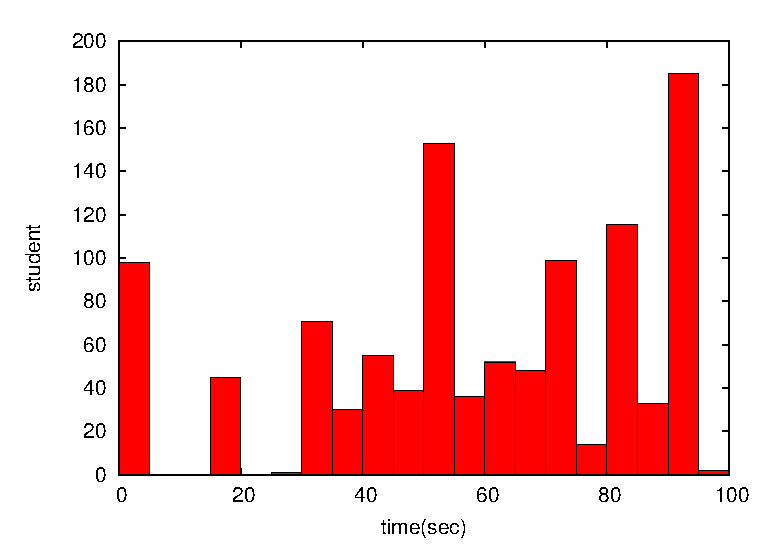
\includegraphics[bb=0 0 390 248,clip,width=\hsize]{oMo12_hist.eps}   
\caption{本実験1:春学期月曜午前}                              
\label{oMo12}                                
\end{center}                                    
\end{minipage}                                 
\begin{minipage}{0.5\hsize}                                            
\begin{center}                              
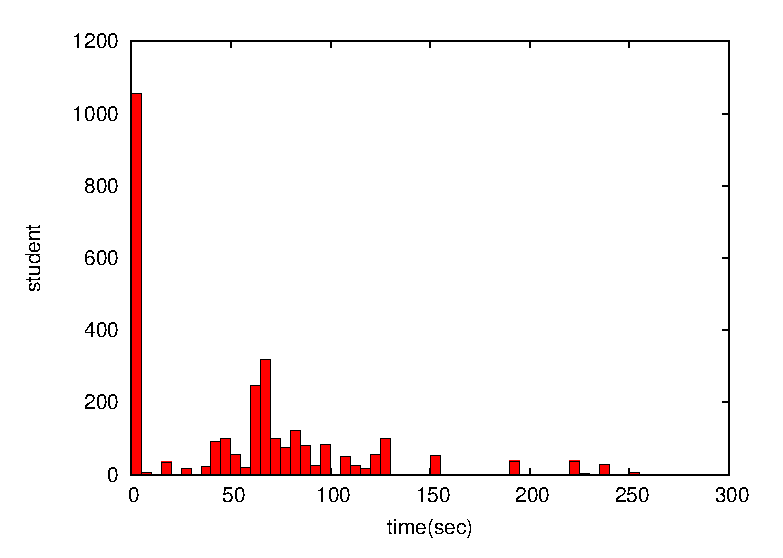
\includegraphics[bb=0 0 390 248,clip,width=\hsize]{oMo345_hist.eps}   
\caption{本実験1:春学期月曜午後}                              
\label{oMo345}                                
\end{center}                                    
\end{minipage}                                 
\end{figure}                                 

\begin{figure}[htpb]                        
\begin{minipage} {0.5\hsize}                             
\begin{center}                              
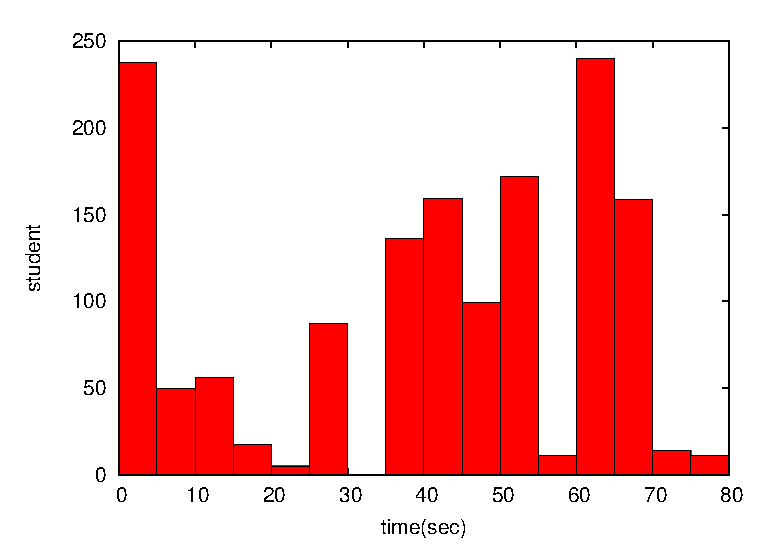
\includegraphics[bb=0 0 390 248,clip,width=\hsize]{oTu12_hist.eps}   
\caption{本実験1:春学期火曜午前}                              
\label{oTu12}                                
\end{center}                                    
\end{minipage}                                 
\begin{minipage}{0.5\hsize}                                            
\begin{center}                              
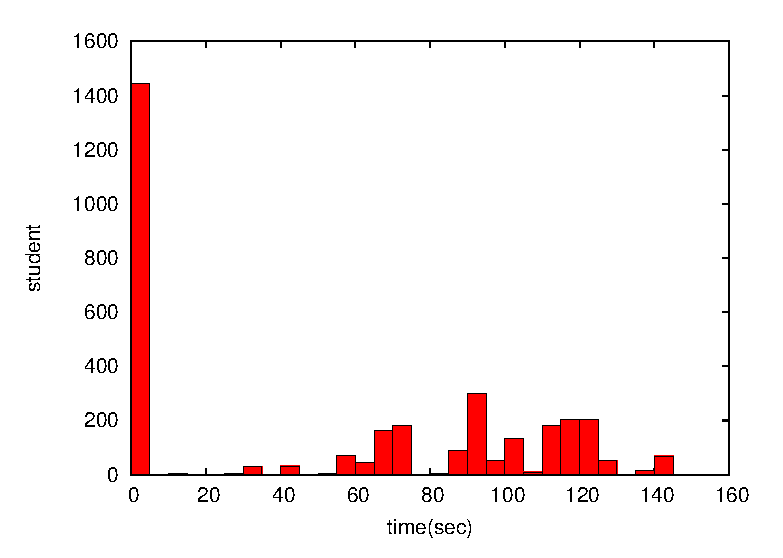
\includegraphics[bb=0 0 390 248,clip,width=\hsize]{oTu345_hist.eps}   
\caption{本実験1:春学期火曜午後}                              
\label{oTu345}                                
\end{center}                                    
\end{minipage}                                 
\end{figure}                                 

\begin{figure}[htpb]                        
\begin{minipage} {0.5\hsize}                             
\begin{center}                              
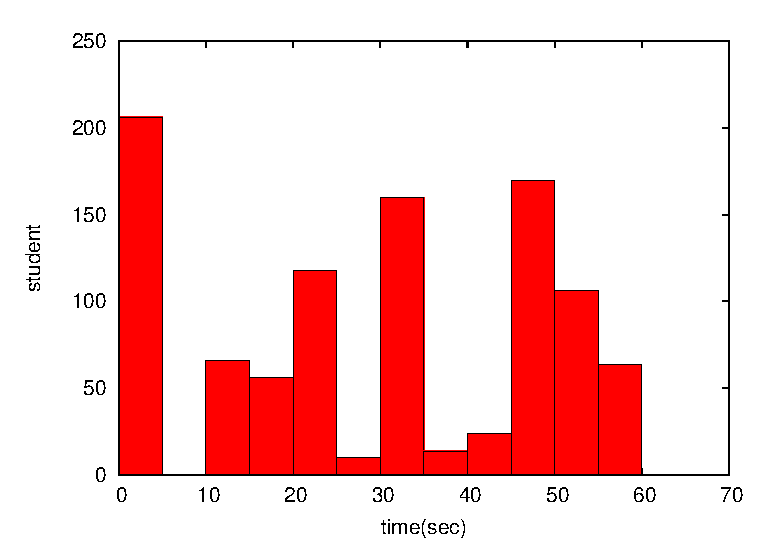
\includegraphics[bb=0 0 390 248,clip,width=\hsize]{oWe12_hist.eps}   
\caption{本実験1:春学期水曜午前}                              
\label{oWe12}                                
\end{center}                                    
\end{minipage}                                 
\begin{minipage}{0.5\hsize}                                            
\begin{center}                              
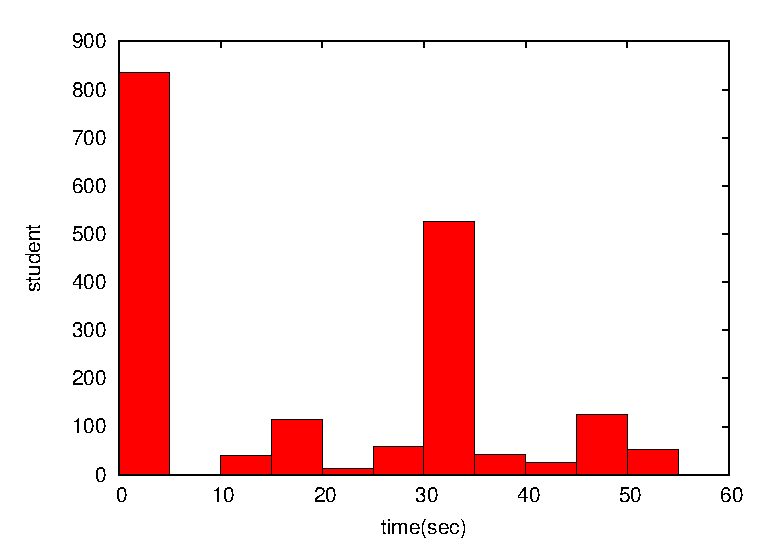
\includegraphics[bb=0 0 390 248,clip,width=\hsize]{oWe345_hist.eps}   
\caption{本実験1:春学期水曜午後}                              
\label{oWe345}                                
\end{center}                                    
\end{minipage}                                 
\end{figure}                                 

\begin{figure}[htpb]                        
\begin{minipage} {0.5\hsize}                             
\begin{center}                              
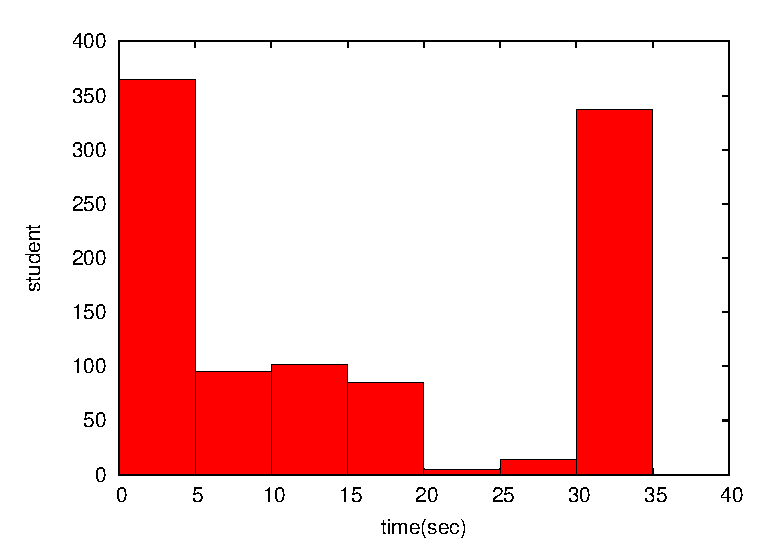
\includegraphics[bb=0 0 390 248,clip,width=\hsize]{oTh12_hist.eps}   
\caption{本実験1:春学期木曜午前}                              
\label{oTh12}                                
\end{center}                                    
\end{minipage}                                 
\begin{minipage}{0.5\hsize}                                            
\begin{center}                              
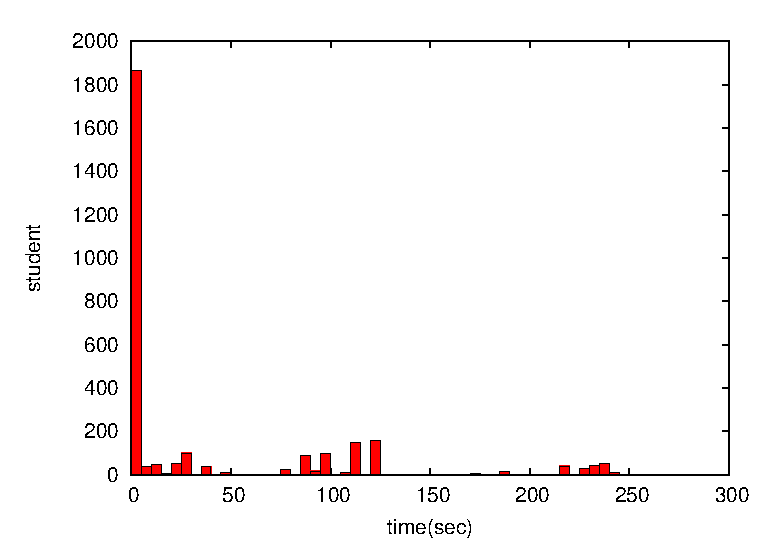
\includegraphics[bb=0 0 390 248,clip,width=\hsize]{oTh345_hist.eps}   
\caption{本実験1:春学期木曜午後}                              
\label{oTh345}                                
\end{center}                                    
\end{minipage}                                 
\end{figure}                                 

\begin{figure}[htpb]                        
\begin{minipage} {0.5\hsize}                             
\begin{center}                              
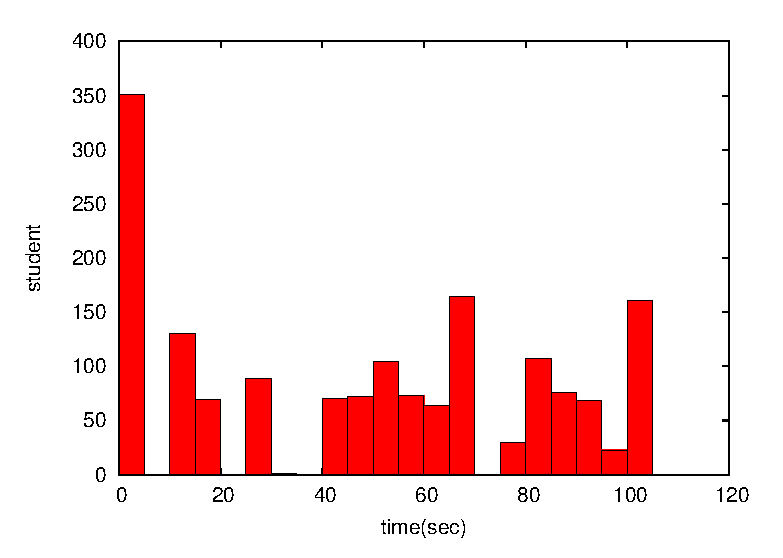
\includegraphics[bb=0 0 390 248,clip,width=\hsize]{oFr12_hist.eps}   
\caption{本実験1:春学期金曜午前}                              
\label{oFr12}                                
\end{center}                                    
\end{minipage}                                 
\begin{minipage}{0.5\hsize}                                            
\begin{center}                              
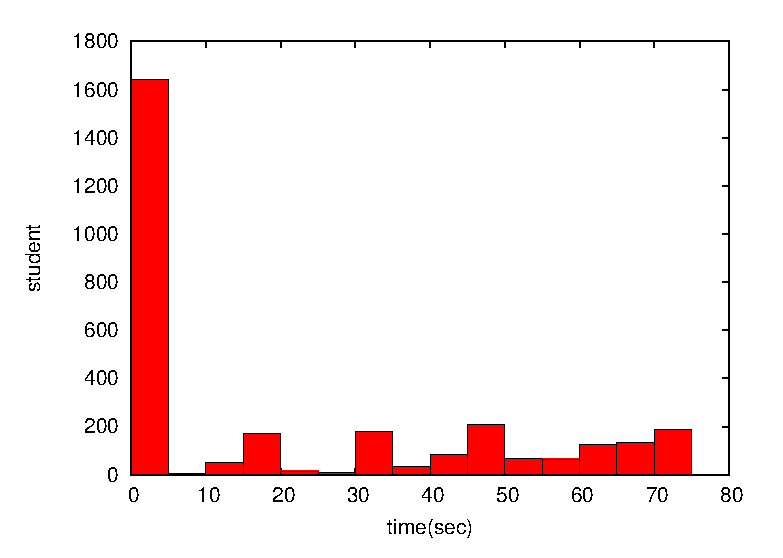
\includegraphics[bb=0 0 390 248,clip,width=\hsize]{oFr345_hist.eps}   
\caption{本実験1:春学期金曜午後}                              
\label{oFr345}                                
\end{center}                                    
\end{minipage}                                 
\end{figure}                                 

\begin{figure}[htpb]                        
\begin{minipage} {0.5\hsize}                             
\begin{center}                              
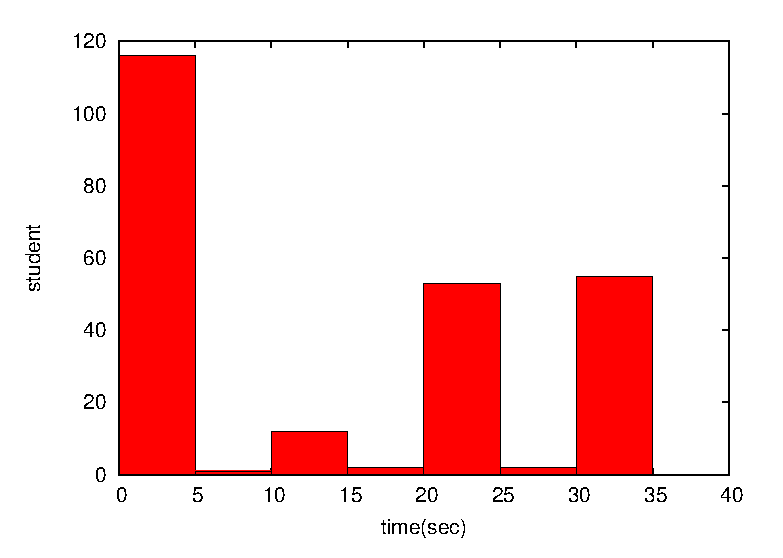
\includegraphics[bb=0 0 390 248,clip,width=\hsize]{oSa12_hist.eps}   
\caption{本実験1:春学期土曜午前}                              
\label{oSa12}                                
\end{center}                                    
\end{minipage}                                 
\begin{minipage}{0.5\hsize}                                            
\begin{center}                              
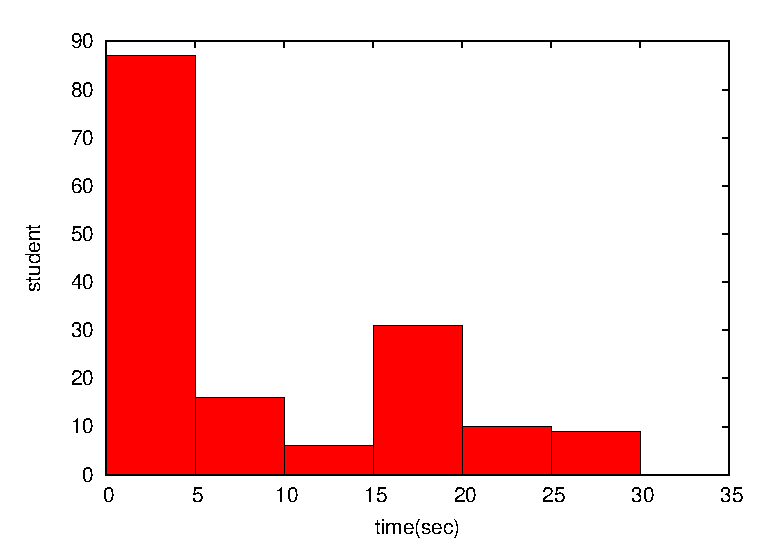
\includegraphics[bb=0 0 390 248,clip,width=\hsize]{oSa345_hist.eps}   
\caption{本実験1:春学期土曜午後}                              
\label{oSa345}                                
\end{center}                                    
\end{minipage}                                 
\end{figure}                                 

%\end{document}

%%%%% End of file %%%%%


\if0
\documentclass[a4paper,10pt]{jarticle}
\usepackage[dvips]{graphicx}
\usepackage{amsmath}

\begin{document}
\fi

\begin{figure}[htpb]                        
\begin{minipage} {0.5\hsize}                             
\begin{center}                              
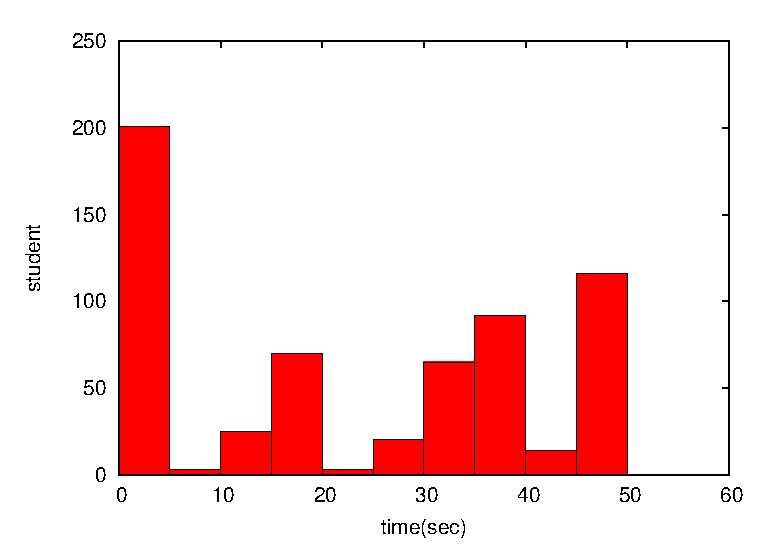
\includegraphics[bb=0 0 390 248,clip,width=\hsize]{xMo12_hist.eps}   
\caption{本実験1:秋学期月曜午前}                              
\label{xMo12}                                
\end{center}                                    
\end{minipage}                                 
\begin{minipage}{0.5\hsize}                                            
\begin{center}                              
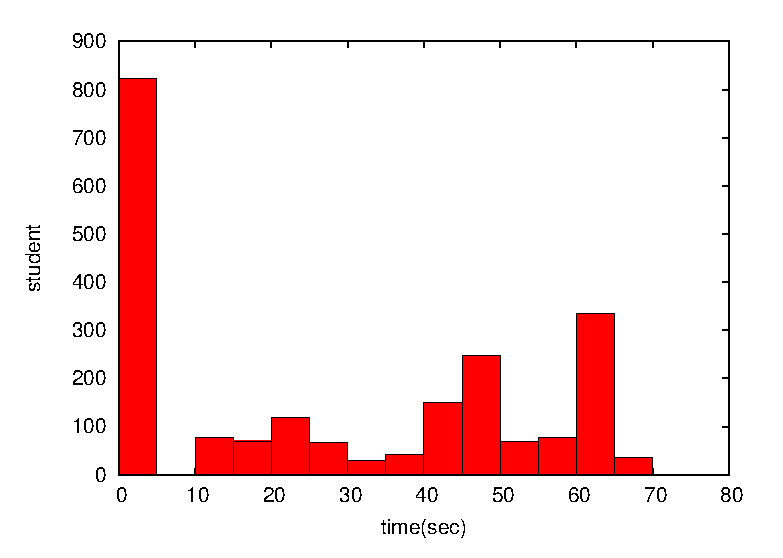
\includegraphics[bb=0 0 390 248,clip,width=\hsize]{xMo345_hist.eps}   
\caption{本実験1:秋学期月曜午後}                              
\label{xMo345}                                
\end{center}                                    
\end{minipage}                                 
\end{figure}                                 

\begin{figure}[htpb]                        
\begin{minipage} {0.5\hsize}                             
\begin{center}                              
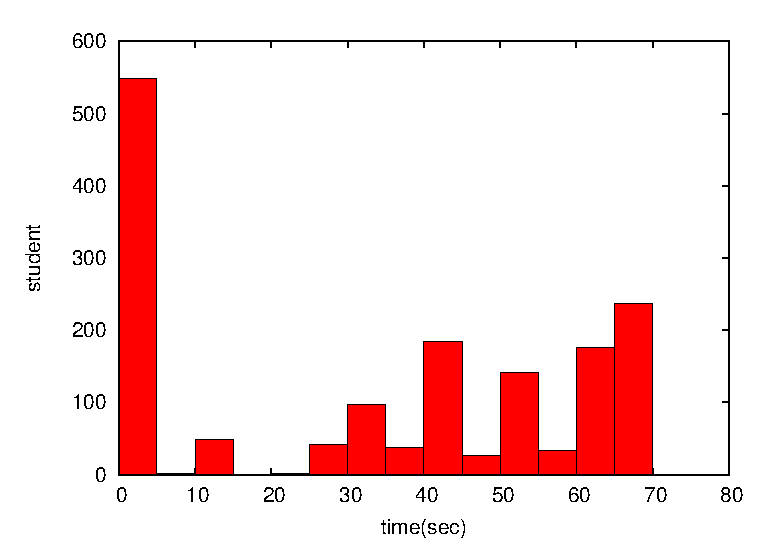
\includegraphics[bb=0 0 390 248,clip,width=\hsize]{xTu12_hist.eps}   
\caption{本実験1:秋学期火曜午前}                              
\label{xTu12}                                
\end{center}                                    
\end{minipage}                                 
\begin{minipage}{0.5\hsize}                                            
\begin{center}                              
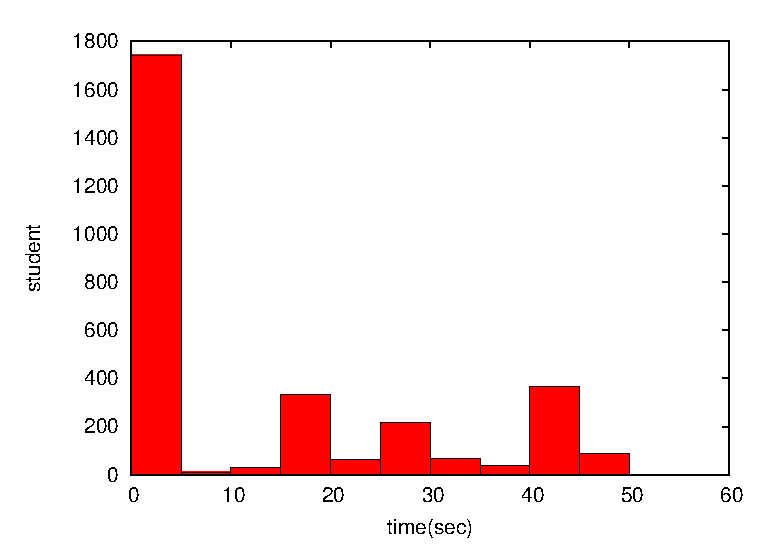
\includegraphics[bb=0 0 390 248,clip,width=\hsize]{xTu345_hist.eps}   
\caption{本実験1:秋学期火曜午後}                              
\label{xTu345}                                
\end{center}                                    
\end{minipage}                                 
\end{figure}                                 

\begin{figure}[htpb]                        
\begin{minipage} {0.5\hsize}                             
\begin{center}                              
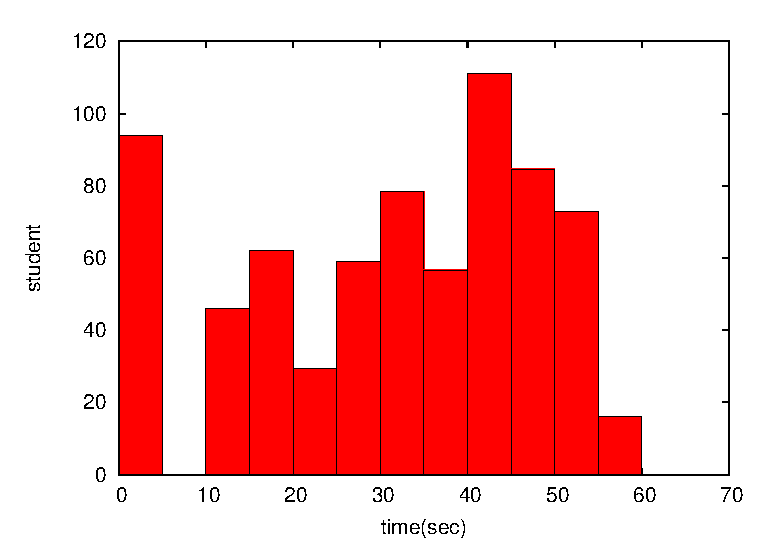
\includegraphics[bb=0 0 390 248,clip,width=\hsize]{xWe12_hist.eps}   
\caption{本実験1:秋学期水曜午前}                              
\label{xWe12}                                
\end{center}                                    
\end{minipage}                                 
\begin{minipage}{0.5\hsize}                                            
\begin{center}                              
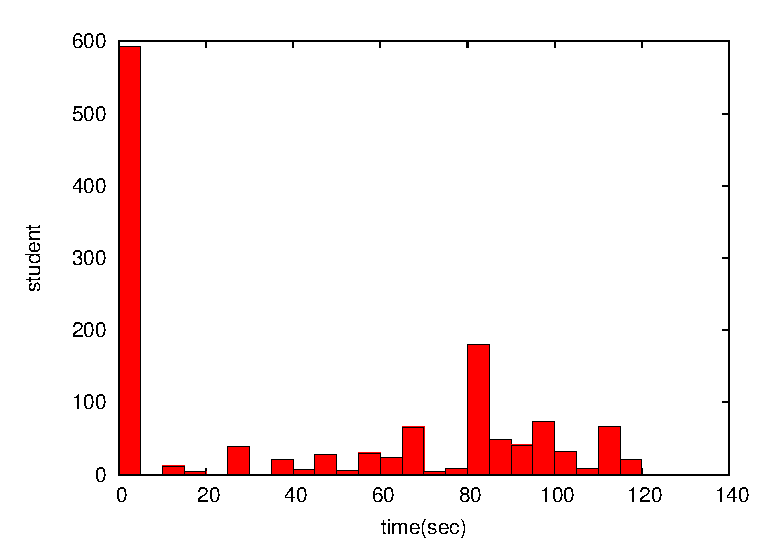
\includegraphics[bb=0 0 390 248,clip,width=\hsize]{xWe345_hist.eps}   
\caption{本実験1:秋学期水曜午後}                              
\label{xWe345}                                
\end{center}                                    
\end{minipage}                                 
\end{figure}                                 

\begin{figure}[htpb]                        
\begin{minipage} {0.5\hsize}                             
\begin{center}                              
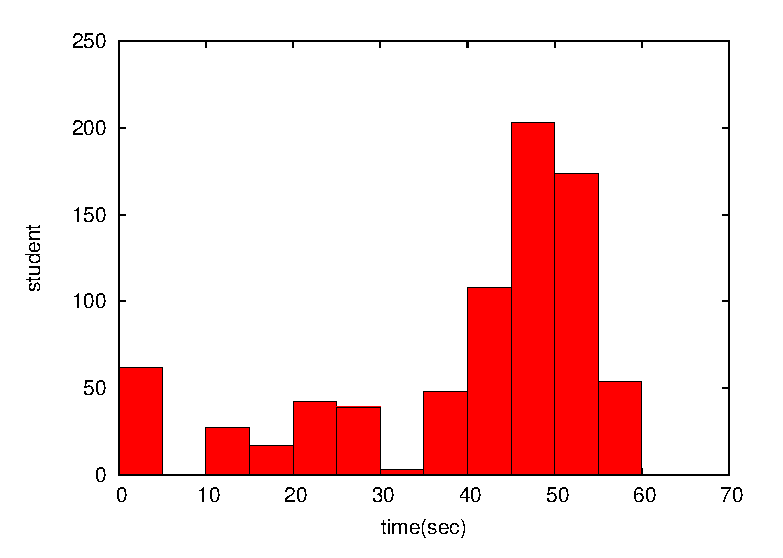
\includegraphics[bb=0 0 390 248,clip,width=\hsize]{xTh12_hist.eps}   
\caption{本実験1:秋学期木曜午前}                              
\label{xTh12}                                
\end{center}                                    
\end{minipage}                                 
\begin{minipage}{0.5\hsize}                                            
\begin{center}                              
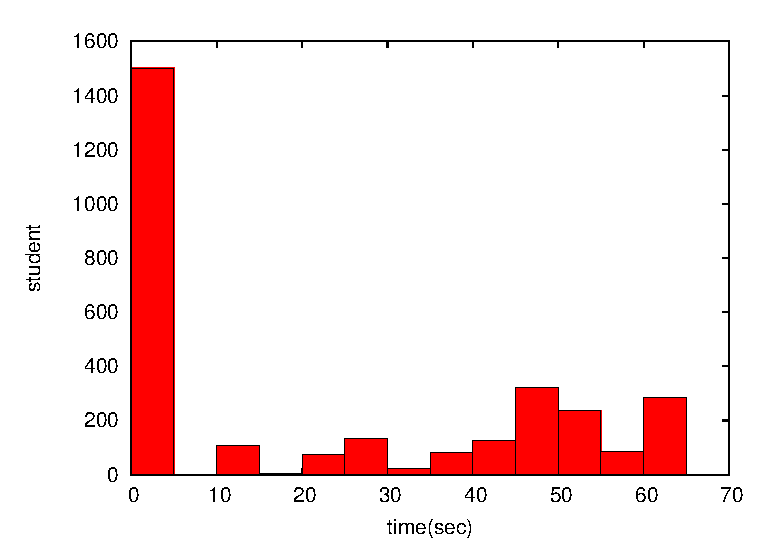
\includegraphics[bb=0 0 390 248,clip,width=\hsize]{xTh345_hist.eps}   
\caption{本実験1:秋学期木曜午後}                              
\label{xTh345}                                
\end{center}                                    
\end{minipage}                                 
\end{figure}                                 

\begin{figure}[htpb]                        
\begin{minipage} {0.5\hsize}                             
\begin{center}                              
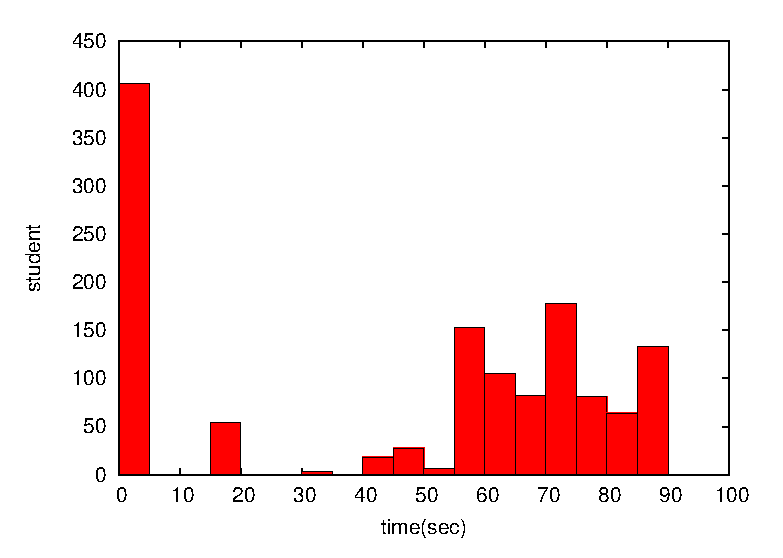
\includegraphics[bb=0 0 390 248,clip,width=\hsize]{xFr12_hist.eps}   
\caption{本実験1:秋学期金曜午前}                              
\label{xFr12}                                
\end{center}                                    
\end{minipage}                                 
\begin{minipage}{0.5\hsize}                                            
\begin{center}                              
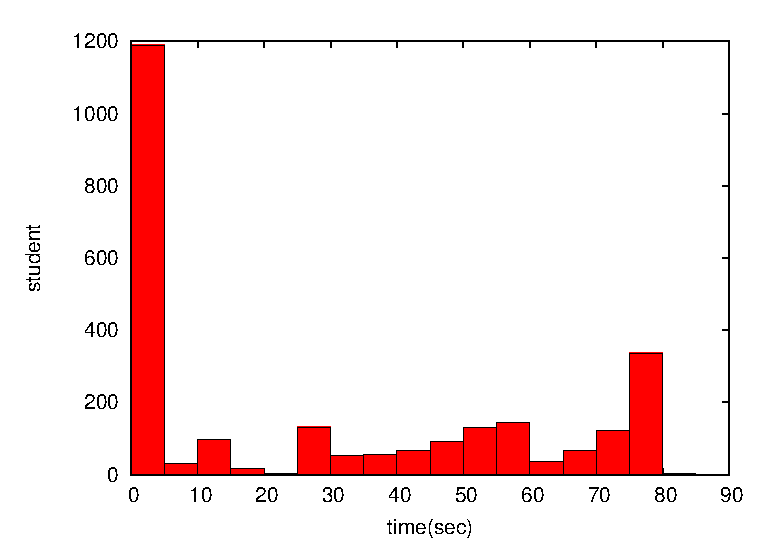
\includegraphics[bb=0 0 390 248,clip,width=\hsize]{xFr345_hist.eps}   
\caption{本実験1:秋学期金曜午後}                              
\label{xFr345}                                
\end{center}                                    
\end{minipage}                                 
\end{figure}                                 

\begin{figure}[htpb]                        
\begin{minipage} {0.5\hsize}                             
\begin{center}                              
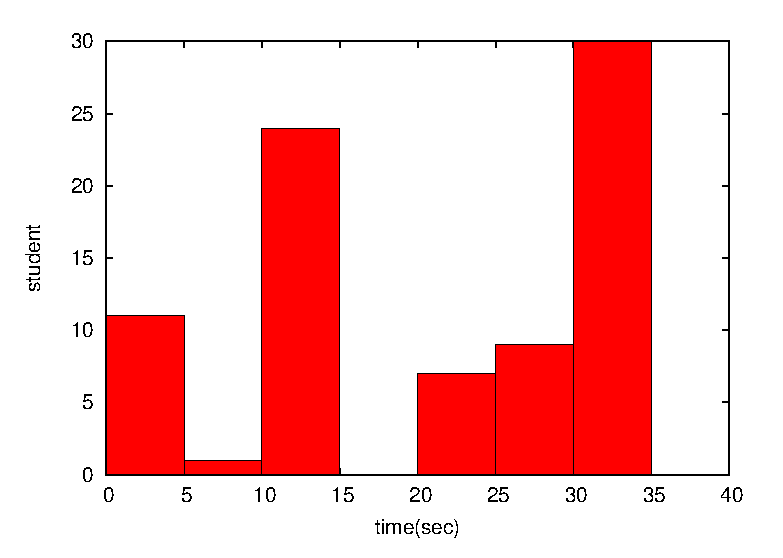
\includegraphics[bb=0 0 390 248,clip,width=\hsize]{xSa12_hist.eps}   
\caption{本実験1:秋学期土曜午前}                              
\label{xSa12}                                
\end{center}                                    
\end{minipage}                                 
\begin{minipage}{0.5\hsize}                                            
\begin{center}                              
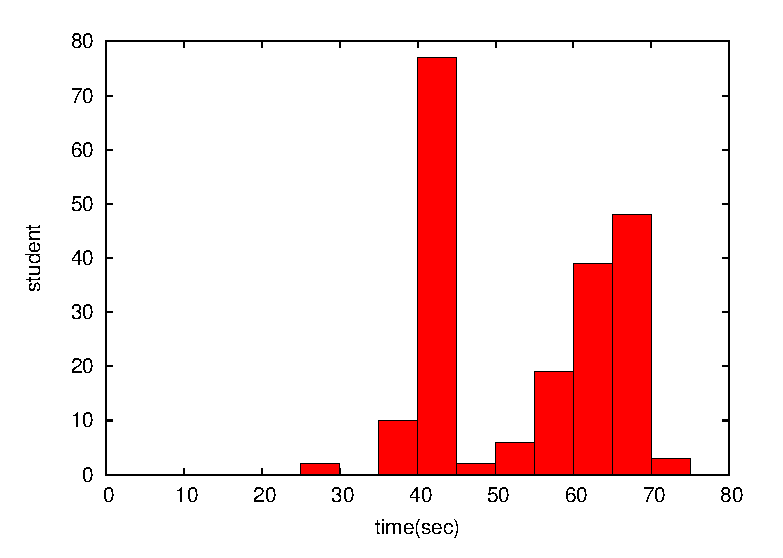
\includegraphics[bb=0 0 390 248,clip,width=\hsize]{xSa345_hist.eps}   
\caption{本実験1:秋学期土曜午後}                              
\label{xSa345}                                
\end{center}                                    
\end{minipage}                                 
\end{figure}                                 

%\end{document}

%%%%% End of file %%%%%


\if0
\documentclass[a4paper,10pt]{jarticle}
\usepackage[dvips]{graphicx}
\usepackage{amsmath}

\begin{document}
\fi

\begin{figure}[htpb]                        
\begin{minipage} {0.5\hsize}                             
\begin{center}                              
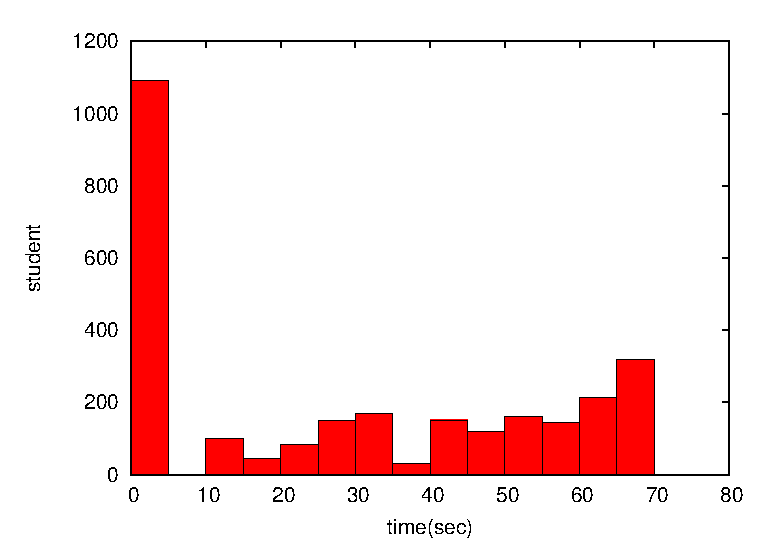
\includegraphics[bb=0 0 390 248,clip,width=\hsize]{oMo345_2_hist.eps}   
\caption{本実験2:春学期月曜午後}                              
\label{oMo345_2}                                
\end{center}                                    
\end{minipage}                                 
\begin{minipage}{0.5\hsize}                                            
\begin{center}                              
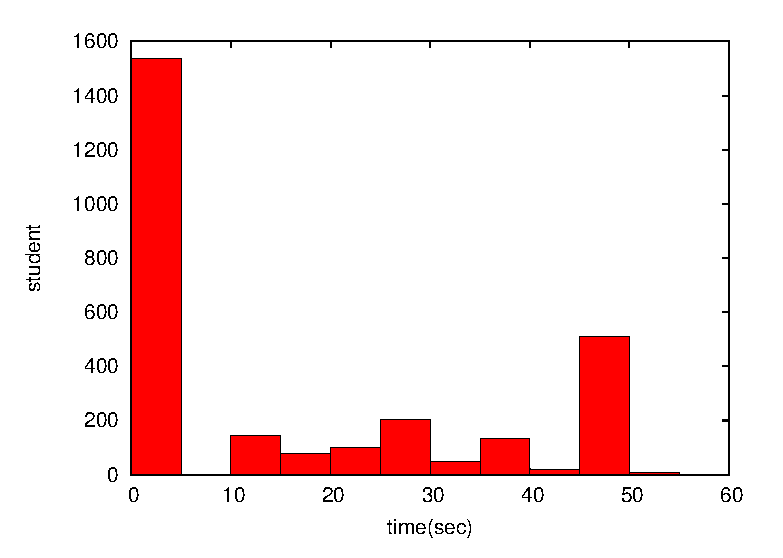
\includegraphics[bb=0 0 390 248,clip,width=\hsize]{oTh345_2_hist.eps}   
\caption{本実験2:春学期木曜午後}                              
\label{oTh345_2}                                
\end{center}                                    
\end{minipage}                                 
\end{figure}                                 

\begin{figure}[htpb]                        
\begin{minipage} {0.5\hsize}                             
\begin{center}                              
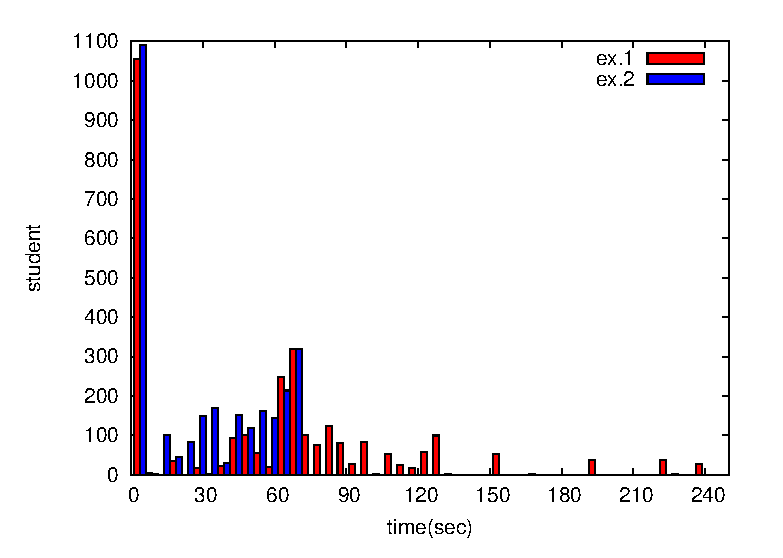
\includegraphics[bb=0 0 390 248,clip,width=\hsize]{omonagahist.eps}   
春学期月曜午後
\end{center}                                    
\end{minipage}                                 
\begin{minipage}{0.5\hsize}                                            
\begin{center}                              
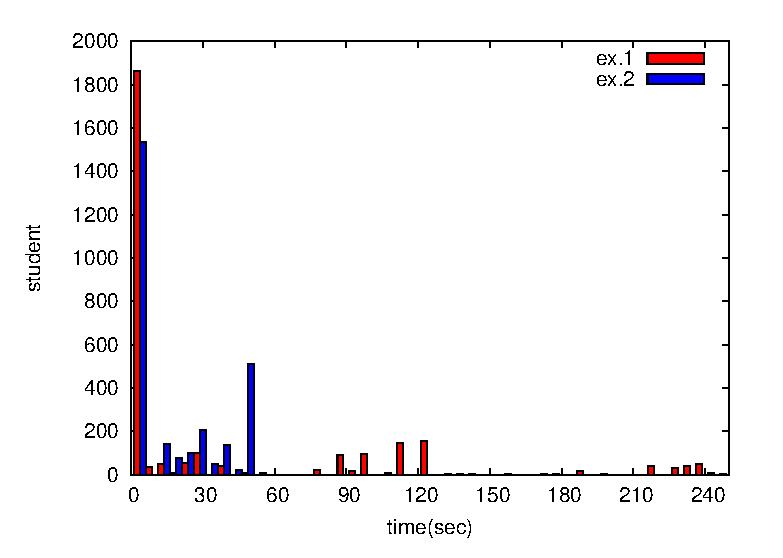
\includegraphics[bb=0 0 390 248,clip,width=\hsize]{otherhist.eps}   
春学期木曜午後
\end{center}                                    
\end{minipage}                                 
\caption{本実験1と本実験2の比較}                              
\label{hikakusiyo}                                
\end{figure}                                 

\begin{figure}[htpb]                        
\begin{minipage} {0.5\hsize}                             
\begin{center}                              
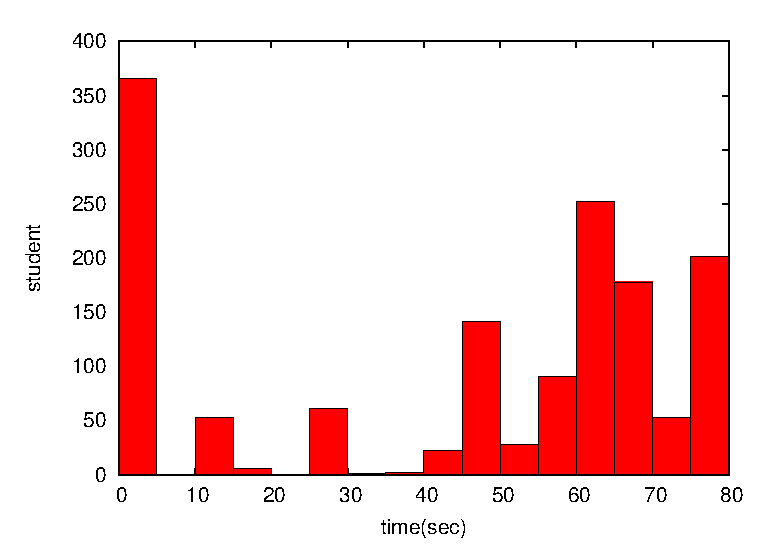
\includegraphics[bb=0 0 390 248,clip,width=\hsize]{oTu12_2_hist.eps}   
\caption{本実験3:春学期火曜午前}                              
\label{oTu12_2}                                
\end{center}                                    
\end{minipage}                                 
\begin{minipage}{0.5\hsize}                                            
\begin{center}                              
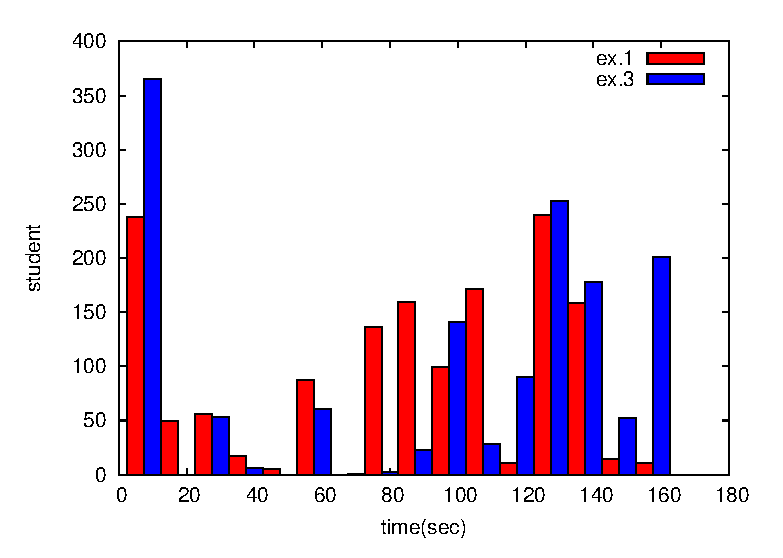
\includegraphics[bb=0 0 390 248,clip,width=\hsize]{otukarehist.eps}   
\caption{本実験1と本実験3の比較}                              
\label{otukaresan}                                
\end{center}                                    
\end{minipage}                                 
\end{figure}                                 

\if0
\begin{figure}[htpb]                        
\begin{minipage} {0.5\hsize}                             
\begin{center}                              
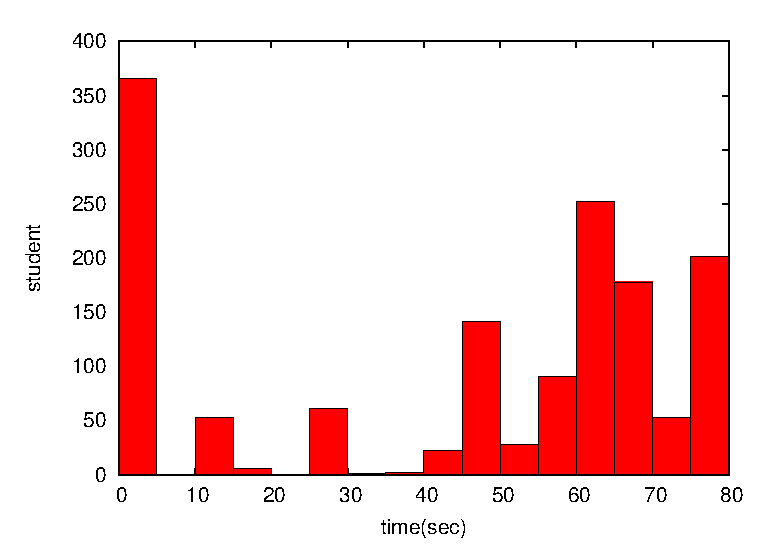
\includegraphics[bb=0 0 390 248,clip,width=\hsize]{oTu12_2_hist.eps}   
\caption{本実験3:春学期火曜午前}                              
\label{oTu12_2}                                
\end{center}                                    
\end{minipage}                                 
\begin{minipage} {0.5\hsize}                             
\end{minipage}                                 
\end{figure}                                 
\fi

%\end{document}

%%%%% End of file %%%%%



\newpage
\section{本実験1と本実験3の教室割当の比較}
表\ref{hikakuotuww}は,本実験1と本実験3の教室割当の結果を比較した表である.
ただし,特殊教室4-0002~4-0021については,授業が割り当てられていないので,省略している. 
\begin{table}[htbp]
\caption{本実験1と本実験3の教室割当の比較}                              
\label{hikakuotuww}
 \begin{center}
\begin{tabular}{c}
  {\footnotesize
  \scalebox{0.8}{


\begin{minipage}{0.5\hsize}
 \begin{center}
本実験1:春学期火曜午前の教室割当
\begin{tabular}{lcc}
   \hline
   room & 1 & 2 \\
   \hline
   4-101 & 65333\_oTu1\_1 & 65143\_oTu2\_1 \\
   4-102 & 65332\_oTu1\_1 & 64426\_oTu2\_1 \\
   4-103 & 65336\_oTu1\_1 & 64426\_oTu2\_2 \\
   4-104 & 65335\_oTu1\_1 & 64426\_oTu2\_3 \\
   4-105 & 64362\_oTu1\_2 & 60153\_oTu2\_1 \\
   4-106 & 62243\_oTu1\_1 & 64105\_oTu2\_1 \\
   4-107 & 64107\_oTu1\_1 & 64420\_oTu2\_1 \\
   4-201A & 65331\_oTu1\_1 &   \\
   4-202 & 60272\_oTu1\_1 & 62120\_oTu2\_2 \\
   4-203 & 65337\_oTu1\_1 & 65145\_oTu2\_1 \\
   4-204 & 60275\_oTu1\_1 & 62745\_oTu2\_1 \\
   4-205 & 60274\_oTu1\_1 & 64459\_oTu2\_1 \\
   4-206 & 64362\_oTu1\_1 & 64316\_oTu2\_1 \\
   4-207 & 62177\_oTu1\_1 & 60197\_oTu2\_1 \\
   4-208 & 62271\_oTu1\_1 & 65183\_oTu2\_1 \\
   4-209 & 62741\_oTu1\_1 & 62120\_oTu2\_4 \\
   4-210 &   & 64409\_oTu2\_1 \\
   4-301 & 60273\_oTu1\_1 & 65144\_oTu2\_1 \\
   4-302 & 65338\_oTu1\_1 & 62341\_oTu2\_1 \\
   4-303 & 62384\_oTu1\_1 & 65255\_oTu2\_1 \\
   4-304 & 62522\_oTu1\_1 & 62523\_oTu2\_1 \\
   4-305 & 62272\_oTu1\_1 & 62595\_oTu2\_1 \\
   4-306 & 62537\_oTu1\_1 & 62120\_oTu2\_3 \\
   4-307 &   & 62581\_oTu2\_1 \\
   4-308 &   & 62505\_oTu2\_1 \\
   4-401 & 62384\_oTu1\_2 & 65182\_oTu2\_1 \\
   4-402 &   &   \\
   4-403 & 64307\_oTu1\_1 & 60157\_oTu2\_1 \\
   4-404 & 60190\_oTu1\_1 & 62351\_oTu2\_1 \\
   4-405 & 62273\_oTu1\_1 & 62120\_oTu2\_1 \\
   4-406 &   & 62173\_oTu2\_1 \\
   4-407 & 64166\_oTu1\_1 &   \\
   4-408 & 64167\_oTu1\_1 & 60815\_oTu2\_1 \\
   4-501 & 65279\_oTu1\_1 & 65120\_oTu2\_1 \\
   4-3101 &   &   \\
   4-3201 &   & 60091\_oTu2\_1 \\
   4-3202 &   &   \\
   4-4A & 62278\_oTu1\_1 & 62278\_oTu2\_1 \\
   4-4B & 64081\_oTu1\_1 & 64081\_oTu2\_1 \\
   4-502 & 62222\_oTu1\_1 & 60145\_oTu2\_1 \\
   4-201B & 65334\_oTu1\_1 &   \\
   4-3401 &   & 65408\_oTu2\_1 \\
   4-3402 & 65415\_oTu1\_1 & 65142\_oTu2\_1 \\
   4-3403 &   &   \\
   4-od1 &   &   \\
   4-od2 & 62167\_oTu1\_1 & 64168\_oTu2\_1 \\
   4-0001 &   & 60452\_oTu2\_1 \\
\if0
   4-0002 &   &   \\
   4-0003 &   &   \\
   4-0004 &   &   \\
   4-0005 &   &   \\
   4-0006 &   &   \\
   4-0007 &   &   \\
   4-0008 &   &   \\
   4-0009 &   &   \\
   4-0010 &   &   \\
   4-0011 &   &   \\
   4-0012 &   &   \\
   4-0013 &   &   \\
   4-0014 &   &   \\
   4-0015 &   &   \\
   4-0016 &   &   \\
   4-0017 &   &   \\
   4-0018 &   &   \\
   4-0019 &   &   \\
   4-0020 &   &   \\
   4-0021 &   &   \\
\fi
   \hline
  \end{tabular}
 \end{center}
\end{minipage}


\begin{minipage}{0.5\hsize}
 \begin{center}
本実験3:春学期火曜午前の教室割当                              
  \begin{tabular}{lcc}
   \hline
   room & 1 & 2 \\
   \hline
   4-101 & 60273\_oTu1\_1 & 65144\_oTu2\_1 \\
   4-102 & 60272\_oTu1\_1 & 62581\_oTu2\_1 \\
   4-103 & 65333\_oTu1\_1 & 65143\_oTu2\_1 \\
   4-104 & 62278\_oTu1\_1 & 62278\_oTu2\_1 \\
   4-105 & 62537\_oTu1\_1 & 62523\_oTu2\_1 \\
   4-106 & 62177\_oTu1\_1 & 62120\_oTu2\_1 \\
   4-107 & 62522\_oTu1\_1 & 65120\_oTu2\_1 \\
   4-201A & 65336\_oTu1\_1 &   \\
   4-202 & 60275\_oTu1\_1 & 64409\_oTu2\_1 \\
   4-203 & 65332\_oTu1\_1 & 62120\_oTu2\_2 \\
   4-204 & 65331\_oTu1\_1 & 62120\_oTu2\_3 \\
   4-205 & 60274\_oTu1\_1 & 65145\_oTu2\_1 \\
   4-206 & 62384\_oTu1\_2 & 62120\_oTu2\_4 \\
   4-207 & 62384\_oTu1\_1 & 60157\_oTu2\_1 \\
   4-208 & 65279\_oTu1\_1 & 60153\_oTu2\_1 \\
   4-209 &   & 62341\_oTu2\_1 \\
   4-210 &   & 62595\_oTu2\_1 \\
   4-301 & 65337\_oTu1\_1 & 64426\_oTu2\_3 \\
   4-302 & 65338\_oTu1\_1 & 64105\_oTu2\_1 \\
   4-303 & 64362\_oTu1\_2 &   \\
   4-304 & 64107\_oTu1\_1 & 64459\_oTu2\_1 \\
   4-305 & 62243\_oTu1\_1 & 60197\_oTu2\_1 \\
   4-306 &   & 62351\_oTu2\_1 \\
   4-307 & 62272\_oTu1\_1 &   \\
   4-308 &   & 65183\_oTu2\_1 \\
   4-401 & 64362\_oTu1\_1 & 64426\_oTu2\_1 \\
   4-402 &   & 64426\_oTu2\_2 \\
   4-403 & 62273\_oTu1\_1 & 62173\_oTu2\_1 \\
   4-404 & 64307\_oTu1\_1 & 60815\_oTu2\_1 \\
   4-405 & 62271\_oTu1\_1 & 65142\_oTu2\_1 \\
   4-406 & 64167\_oTu1\_1 & 64420\_oTu2\_1 \\
   4-407 & 60190\_oTu1\_1 & 60091\_oTu2\_1 \\
   4-408 & 64081\_oTu1\_1 & 64081\_oTu2\_1 \\
   4-501 & 62222\_oTu1\_1 & 64316\_oTu2\_1 \\
   4-3101 &   & 62505\_oTu2\_1 \\
   4-3201 &   &   \\
   4-3202 &   &   \\
   4-4A & 65415\_oTu1\_1 &   \\
   4-4B &   & 65408\_oTu2\_1 \\
   4-502 &   & 60145\_oTu2\_1 \\
   4-201B & 65334\_oTu1\_1 &   \\
   4-3401 & 64166\_oTu1\_1 & 65255\_oTu2\_1 \\
   4-3402 & 62741\_oTu1\_1 & 62745\_oTu2\_1 \\
   4-3403 & 65335\_oTu1\_1 & 65182\_oTu2\_1 \\
   4-od1 &   &   \\
   4-od2 & 62167\_oTu1\_1 & 64168\_oTu2\_1 \\
   4-0001 &   & 60452\_oTu2\_1 \\
\if0
   4-0002 &   &   \\
   4-0003 &   &   \\
   4-0004 &   &   \\
   4-0005 &   &   \\
   4-0006 &   &   \\
   4-0007 &   &   \\
   4-0008 &   &   \\
   4-0009 &   &   \\
   4-0010 &   &   \\
   4-0011 &   &   \\
   4-0012 &   &   \\
   4-0013 &   &   \\
   4-0014 &   &   \\
   4-0015 &   &   \\
   4-0016 &   &   \\
   4-0017 &   &   \\
   4-0018 &   &   \\
   4-0019 &   &   \\
   4-0020 &   &   \\
   4-0021 &   &   \\
\fi
   \hline
  \end{tabular}
 \end{center}
\end{minipage}



}  }
  \end{tabular}
 \end{center}
\end{table}
%\multicolumn{1}{l}{※特殊教室4-0002~4-0021については,授業が割り当てられていないので,省略している.} 





\end{document}





